%Define style
\documentclass[11pt,a4paper,final]{report}
%Set reduced margins
%\usepackage[margin=25mm]{geometry}
\usepackage{geometry}
\geometry{a4paper,
  twoside,
  margin=20mm,
  bindingoffset=20mm, %Extra margin on binding edge (must total 40mm)
  top=25mm, %Override top margin
  bottom=25mm, %Override bottom margin
  heightrounded,
}

% Use fancy headers
\usepackage{fancyhdr}
%\pagestyle{fancy}
\pagestyle{headings}

%Set line spacing to 1.5 except captions etc
\usepackage{setspace} 
%\doublespacing
\onehalfspacing

%Reduce font size for figure captions
\usepackage[font=small,labelfont=bf, textfont=it]{caption}

%Enable graphics
\usepackage{graphicx}

%Enable coloured text
\usepackage{xcolor}

%Enable floats (ie. aligning of multi-line equations)
\usepackage{float}

%Enable equations package
\usepackage{amsmath}

%Enable control over section numbering
\usepackage{titlesec}
\setcounter{secnumdepth}{3}

%Enable PDF links
\usepackage[hidelinks]{hyperref}

%Enable SI units package
\usepackage{siunitx}

%Enable inline references
\usepackage{bibentry}
\nobibliography*


%Define way to add matrix vertical line, used in 3D matrices and augmenting
\makeatletter
\renewcommand*\env@matrix[1][*\c@MaxMatrixCols c]{%
	\hskip -\arraycolsep
	\let\@ifnextchar\new@ifnextchar
	\array{#1}}
\makeatother

%Define way to add tensor dots
\def\onedot{$\mathsurround0pt\ldotp$}
\def\cddot{% two dots stacked vertically
	\mathbin{\vcenter{\baselineskip.67ex
		\hbox{\onedot}\hbox{\onedot}}%
	}}%
\def\cdddot#1{% three dots 
	\mathbin{\vcenter{\baselineskip.67ex
		\hbox{\onedot}\hbox{\onedot}\hbox{\onedot}%
	}}%
}

%Title and author info (REDUNDANT WITH CUSTOM TITLE PAGE)
\title{Thesis 2018}
\author{
	Collins, J.T. \\ 
	Department of Physics\\
	University of Bath\\
}

%Include build date
\date{\today}


%Control TOC size
\AtBeginDocument{
  \addtocontents{toc}{\normalsize}
  \addtocontents{lof}{\normalsize}
}

\begin{document}


% Custom title page
\begin{titlepage}
    \begin{center}
    \vspace*{1cm}
    
    \LARGE
    \textbf{Optimising Chiral Dissymmetry\\ in Plasmonic Nanostructures}
    
    \vspace{0.5cm}
    \large
    Confirmation Report
    
    \vspace{1.5cm}
    \normalsize
    \textbf{Joel T. Collins}\\
    \textbf{Supervisor: }V. K. Valev
    
    \vspace{0.8cm}
    Department of Physics\\
    University of Bath
    
    \vspace{0.5cm}
    \today
    
    \vspace{1.5cm}
\end{center}
\end{titlepage}

% Abstract
\begin{abstract}
	\setcounter{page}{0}  % Fix the janky page numbering to get the correct binding-edge margin
    Nonlinear optical processes provide a valuable technique for probing properties of chiral structures, those lacking mirror symmetry. 
Such structures are encountered frequently throughout organic chemistry, pharmacology, and biology, with a recent growing emphasis on sensitive characterisation of small quantities of chiral molecules. 
	    
It has been shown that chiroptical effects such as circular dichroism and optical rotation are significantly enhanced in second-harmonic generation. 
Additionally, plasmonic nanostructures can create local regions of high intensity, highly chiral electromagnetic fields that further enhance chiroptical interactions with molecules attached to the material surface. 
	    
In this report, chiroptical and nonlinear optical properties of dielectric materials are reviewed in the context of both natural media and plasmonic nanomaterials. 
Using these principles, three novel chiral analysis schemes are experimentally demonstrated. Each experiment is designed for the characterisation of a unique plasmonic nanomaterial, all making use of enhanced nonlinear chiroptical effects. We first consider plasmonic structures with dimensions comparable to the wavelength of incident light. In these structures, electric field hotspots form, leading to small regions of enhanced chiral and nonlinear optical interactions. A theoretical description making use of a modal analysis and group theory is found to well match experimental results. Following this, we consider the effects of anisotropy on nonlinear chiroptical measurements of planar nanomaterials. The structures are of sub-wavelength dimensions, however exhibit strong anisotropy that can contribute to chiroptical effects. We demonstrate that specific experimental configurations can be exploited to separate the contributions from structural chirality and anisotropy, allowing pure chiral information to be obtained from highly anisotropic materials. Finally, we consider the case of removing structural anisotropy by dispersing anisotropic nanostructured in liquid. In this case, nonlinear scattering is measured, and found to exhibit strong chiroptical effects. This is the first experimental report of second-harmonic scattering circular difference, and demonstrates significantly enhanced sensitivity when compared to more widely used linear characterisation techniques.

By designing new experimental schemes considering the unique challenges associated with each nanomaterial geometry, previously unobserved optical properties of the materials are revealed. Such tailored experimental methods pave the way for the further optimisation of chiral nanomaterials designed for nanorobotic, photonic devices, and chemical sensing applications.
\end{abstract}
\clearpage

\pagenumbering{arabic}  % Start normal page numbering
% Table of contents
\clearpage 
\tableofcontents
\clearpage


% Acknowledgements
\chapter*{Acknowledgements}

\color{red}
I'd like to thank \LaTeX  for not being quite as horrible to use as MS Word.

\noindent\textbf{Notes to self:}

\noindent SyncTeX should be installed separately to function in VS Code. \\
Install from choco
\begin{verbatim}
	https://chocolatey.org/packages/synctex
\end{verbatim}
or download from TeXLive 
\begin{verbatim}
	https://www.tug.org/svn/texlive/trunk/Master/bin/win32/
\end{verbatim}
then place synctex.exe and kpathsea***.dll in /Program Files/MiKTeX 2.9/miktex/bin/x64/.

\noindent To make SumatraPDF work with inverse-search, set Sumatra inverse search command (in Sumatra settings) to 
\begin{verbatim}
"C:\Program Files\Microsoft VS Code\Code.exe" -g "%f:%l"
\end{verbatim}

\noindent To make Sumatra work with forward-search, add to user or workspace settings
\begin{verbatim}
	"latex-workshop.view.pdf.external.synctex": {
		"command": "SumatraPDF",
		"args": [
			"-forward-search",
			"%TEX%",
			"%LINE%",
			"-reuse-instance",
			"-inverse-search",
			"\"code.exe\" -g \"%f:%l\"",
			"%PDF%",
		]
	},
\end{verbatim}

\clearpage

\noindent\textbf{To-do:}
\begin{itemize}
	\item Add introduction paragraphs to start of each paper section, linking it to the previous paper
	\item Discuss broad LSP resonance in nanohelix papers
	\item Add additional discussion/data of failed methods etc. (eg additional nanohelix data)
	\item Split oversized figures where it would make sense
	\item Rewrite abstract
    \item Actually write a thesis
\end{itemize}
\color{black}

% Publications
\chapter*{Publications}

\bibentry{Collins2018b}

\bigskip \noindent \bibentry{Kuppe2018}

\bigskip \noindent \bibentry{Collins2018}

\bigskip \noindent \bibentry{Collins2017}

\bigskip \noindent \bibentry{Hooper2017}


% Main text
%\chapter{Structure and Overview}\label{sec:background:Introduction}
\color{red}

\begin{itemize}
    \item Understanding chirality is important (ref section)
    \item Chemicals have been used to understand chirality (ref section)
    \item However, nanomaterials can be better (ref section)
    \item Mention that bits of the background sections are lifted from my parts of the review paper
    \item Briefly introduce some work not discussed in the thesis
    \item Mention microscopy work with Dave Carbery.
\end{itemize}
\color{black}

Time has also been spent developing Python libraries to simplify data acquisition and analysis on a range of experimental setups within the group. While not discussed in this thesis, diffraction CID experiments undertaken by C. Kuppe (reference~\cite{Kuppe2018}) made use of an experiment-automation library I developed during this project, and eventually merged into a larger library, detailed in appendix~\ref{sec:appendix:labdo}. Data analysis shown in section~\ref{sec:results:OAinPlanarNanohelices} made use of another Python library I developed to automate the filtering, processing, and plotting of data from our SHG optical activity setup. The library, detailed in appendix~\ref{sec:appendix:pyshg}, has since been used in submitted work by D. C. Hooper, and is expected to be used in similar experiments going forward.
\chapter{Chirality}\label{sec:background:Chirality}

Chirality has historically been defined as any shape whose mirror-image cannot be superimposed onto itself by only rotation, based on the 1894 definition by Lord Kelvin~\cite{Kelvin1894}. 
A more comprehensive definition accounting for both temporal and spatial symmetry was proposed in 1986 by Barron~\cite{Barron1986}, stating that ``true chirality is exhibited by systems that exist in two distinct enantiomeric states that are interconverted by space inversion, but not by time reversal combined with any proper spatial rotation.''
The word chiral derives from a Greek word for ``the hand'', an archetypal example of a chiral structure. A chiral pair of structures, ``enantiomorphs'', are often referred to as ``left-handed'' and ``right-handed'' because of this historical relationship to the hand. While chirality is very much present in nature on a macroscopic scale, from the structure of cyclones to the helicity of most gastropod shells, it is crucially exhibited by almost all biochemically and many pharmaceutically important molecules: the helical structure of DNA being a famous example of the importance of chirality in biology. Further, amino acids on earth are almost all exclusively ``left-handed'' chiral, while sugars are almost exclusively ``right-handed'' chiral. Importantly, while chiral molecules are energetically identical unless considering the weak interaction, their opposite enantiomorphs (``enantiomers'' for molecules) can exhibit dramatically different effects on living organisms. 
A tragically famous example is the pharmaceutical drug Thalidomide. One enantiomer functions as an effective relief medication for morning-sickness, while the other can cause severe birth defects~\cite{Vargesson2015}. Any contamination of the wrong enantiomer can dramatically change the medical properties of the drug.
Another example is methamphetamine (methylamphetamine). One enantiomer (\textit{l-}methamphetamine) has been used as the, relatively benign, active ingredient in nasal decongestants in the United States~\cite{Mendelson2008}. Conversely, the other enantiomer (\textit{d-}methamphetamine, commonly ``crystal meth'') ``exerts potent physiological and psychostimulant effects and has high abuse liability''~\cite{Nishimura2017}. 
Similarly, ketamine is a racemic mixture of the enantiomers \textit{d-}ketamine and \textit{l-}ketamine, used for anaesthesia and pain relief, but commonly exhibiting hallucinogenic side effects~\cite{Craven2007}. Studies have established, however, that the analgesic effects are significantly more potent in one enantiomer, whereas the hallucinogenic side-effects are predominantly the result of the other enantiomer~\cite{Craven2007, Muller2016, Zeilhofer1992}. 
Obtaining either enantiomer over the other has clear advantages over the production and use of racemic mixtures. Typically enantioseparation is performed in-situ, and involves the selective removal of one enantiomer from the racemic mixture until an acceptable ratio is achieved~\cite{Nguyen2006}. There is thus a prevailing need for robust characterisation techniques of chiral systems within the pharmaceutical industry and biochemical research. 
Beyond biomolecular systems, man-made chiral structures (discussed further in section~\ref{sec:background:Plasmonics}) can be fabricated for applications in photonic devices~\cite{Rizza2015, Esposito2016, Hou2016}, nanorobotics~\cite{Urban2015, Schamel2013a}, and in particular chemical sensing platforms. Common between these applications, biochemical research, and pharmaceutical manufacturing, is the need for comprehensive experimental characterisation of chiral systems. Generally, chiral information can be obtained from any interaction between the chiral structure with unknown properties, and a well understood chiral system responsible for sensing. Enantioselective processes can occur, for example, from interactions between two chiral molecules, or more relevant to this work, interactions between chiral structures and light. We can describe the interaction between light and a general chiral material by considering the polarisation properties of a propagating monochromatic plane wave through a chiral medium.

The general mathematical form of a coherent monochromatic plane wave at a distance $z$ and time $t$, oscillating at a frequency $\omega$, is given by equation~\ref{eq:background:chirality:generalwave}. The wave is polarised in the $x-y$ plane, and propagates along the $z$ axis with a wavevector $k_z$. $\phi$ describes the relative phase shift between the orthogonal components of polarisation, oscillating in the $\mathbf{\hat{x}}$ and $\mathbf{\hat{y}}$ directions with amplitudes $E_x$ and $E_y$ respectively.
\begin{equation} \label{eq:background:chirality:generalwave}
    \mathbf{E}= E_x  \mathbf{\hat{x}} \cos(k_z z-\omega t) - E_y \mathbf{\hat{y}} \cos(k_z z-\omega t +\phi)
\end{equation}
Linear combinations of $E_x$ and $E_y$, as in equation~\ref{eq:background:chirality:generalwave}, with no phase shift ($\phi=0$) result in linearly polarised light, with a polarisation axis depending on the relative amplitudes of $E_x$ and $E_y$. Crucially, linear combinations of $E_x$ and $E_y$ with non-zero amplitudes and a non-zero phase shift $\phi$ will result in a chiral polarisation state: the polarisation vector rotates about the axis of propagation, tracing a helical profile. The ellipticity of this wave depends on both the phase and amplitude of the orthogonal linear components $E_x$ and $E_y$. Circular polarisation is the special case of a $\pm \pi/2$ phase shift between $E_x$ and $E_y$ of equal amplitude. The sign of the phase shift determines the direction of the polarisation rotation, resulting in left- and right-circularly polarised light (CPL). In this work, right-circularly polarised (RCP) light is defined as a clockwise rotation of the polarisation vector \textit{from the point of view of the wave source}. Conversely, left-circularly polarised (LCP) light is defined as a counter-clockwise rotation of the polarisation vector in the same frame. The wave equations for left- and right-circularly polarised light in this convention are given by equation~\ref{eq:background:chirality:CPL}~\cite[\S 8.1.2]{Hecht2013}). 
\begin{equation} \label{eq:background:chirality:CPL}
    \begin{split}
        & \mathbf{E}_{RCP} = E_0 \left[ \mathbf{\hat{x}} \cos(k_z z-\omega t) + \mathbf{\hat{y}} \sin(k_z z-\omega t )\right]\\
        & \mathbf{E}_{LCP}= E_0 \left[ \mathbf{\hat{x}} \cos(k_z z-\omega t) - \mathbf{\hat{y}} \sin(k_z z-\omega t )\right]
    \end{split}
\end{equation}
Since left- and right-circular polarisation states are orthogonal, any arbitrary polarisation can also be represented by the linear combination of LCP and RCP waves. For example, linear polarisation can be represented as the linear combination of equal amplitude LCP and RCP waves $\mathbf{E}_{LCP}$ and $\mathbf{E}_{RCP}$. 

Outside of the special cases of CPL and linearly polarised light, polarisation is described as elliptical, since both the total field amplitude, and the direction of polarisation, can vary as the wave propagates, resulting in an elliptical profile. The orientation of the elliptical profile, the ellipticity of the profile, and the direction of polarisation rotation, all depend on both the amplitudes of $E_x$ and $E_y$, and the phase between them.
Experimentally, elliptical and circular polarisations of light are realised by making use of an anisotropic, birefringent medium: one which has different refractive indices in orthogonal axes. Anisotropy in the real part of refractive index means that components of light polarised along the orthogonal axes, known as the medium's fast and slow axes, propagate with different phase velocities and accumulate a relative phase shift during propagation. By designing the thickness of the material such that the accumulated phase shift is $2m\pi \pm \pi/2$ at the operating wavelength $\lambda$ (where $m$ is some integer), elliptically and circularly polarised light can be obtained. Such a device is known as a quarter-wave plate (QWP), as it induces a shift of $\lambda/4$ between orthogonal polarisation components. The orientation of the ellipses major axis depends on the direction of the incident polarisation, and the ellipticity depends on the angle of the material's fast axis relative to the direction of incident polarisation (figure~\ref{fig:background:Chirality:QWP}). Similarly, the orientation of linear polarisation can be rotated (known as ``optical rotation'', OR) by making use of a half-wave plate (HWP), which induces a relative phase shift of $2m\pi \pm \pi$ between orthogonal polarisation components. The angle of optical rotation also depends on the angle of the material's fast axis relative to the direction of incident polarisation.
\begin{figure}[htb!]
    \centering
    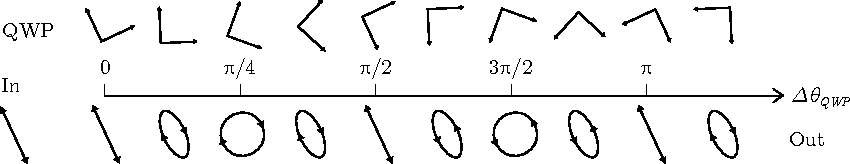
\includegraphics[scale=1.0]{./figures/background/chiroptics/QWP_in_out.pdf}
    \caption{\label{fig:background:Chirality:QWP}Output polarisation from a QWP at an angle $\Delta\theta_{QWP}$ to the input polarisation. The angle of the incident polarisation (and subsequent elliptical and linear outputs) can controlled by a half-wave plate.}
\end{figure}

Whereas linear birefringence results from structural anisotropy, a medium with structural \textit{chirality}, such as a chiral molecular system, can exhibit a similar dissymmetry in its interaction with LCP and RCP light. This leads to chiral-optical (chiroptical) effects, directly beneficial for both polarisation optics, and the characterisation of unknown chiral structures. The rest of this chapter discusses the physical origin of chiroptical effects relevant to this work, and the parameters used to characterise the interactions between chiral structures and light.


\section{Structural Chirality}\label{sec:background:Chirality:Structural}
In the simple case of a linear, isotropic medium, the macroscopic electromagnetic response of the material is described by the constitutive relations given in equation~\ref{eq:background:chirality:isotropicConstitutive}. These relate the material's internal electric displacement field $\bf{\tilde D}$ and magnetic field strength $\bf{\tilde H}$ to external electric and magnetic fields $\bf{\tilde E}$ and $\bf{\tilde B}$, where tildes denote complex values. Here, $\varepsilon$ and $\mu$ are complex scalars and correspond to the isotropic electric permittivity and magnetic permeability of the material.
\begin{equation}\label{eq:background:chirality:isotropicConstitutive}
	\begin{split}
        & \bf{\tilde D} = \tilde \varepsilon \bf{\tilde E} \\
        & \bf{\tilde B} = \tilde \mu \bf{\tilde H}
	\end{split}
\end{equation}
In the general case however, we cannot assume isotropy. Furthermore, $\bf{\tilde D}$ and $\bf{\tilde H}$ may depend on both $\bf{\tilde E}$ and $\bf{\tilde B}$ (magnetoelectric coupling). For a bi-anisotropic medium (anisotropic, with no-zero magnetoelectric coupling), the constitutive relations take the form of equation~\ref{eq:background:chirality:fullConstitutive}.\cite{Ishimaru2003, Capolino2009}. Here, $\bf{\tilde \varepsilon}$, $\bf{\tilde \mu}$, $\bf{\tilde \xi}$, and $\bf{\tilde \zeta}$ are $3 \times 3$ matrices due to the anisotropy of the material. $\bf{\tilde \xi}$, and $\bf{\tilde \zeta}$ are pseudo-scalars (behaving as scalars, but changing sign under parity inversion), and describe the magnetoelectric coupling.
\begin{equation}\label{eq:background:chirality:fullConstitutive}
    \begin{bmatrix}
        \bf{\tilde D} \\
        \bf{\tilde B}
    \end{bmatrix}
    =
    \begin{bmatrix}
        \bf{\tilde \varepsilon} & \bf{\tilde \xi} \\
        \bf{\tilde \zeta} & \bf{\tilde \mu}
    \end{bmatrix}
    \begin{bmatrix}
        \bf{\tilde E} \\
        \bf{\tilde H}
    \end{bmatrix}
\end{equation}
In the case of a non-gyrotropic material (exhibiting no magneto-optic rotation), equation~\ref{eq:background:chirality:fullConstitutive} has additional constraints, due to time-reversal symmetry, given in equation~\ref{eq:background:chirality:nongyroConstraints} \cite{Ishimaru2003}.
\begin{equation}\label{eq:background:chirality:nongyroConstraints}
    \begin{split}
        &[\bf{\tilde \xi}]^t = -[\bf{\tilde \zeta}] \\
        &[\bf{\tilde \varepsilon}]^t = [\bf{\tilde \varepsilon}] \\
        &[\bf{\tilde \mu}]^t = [\bf{\tilde \mu}]
    \end{split}
\end{equation}
The expressions shown in equation~\ref{eq:background:chirality:isotropicConstitutive} are a special case of equation~\ref{eq:background:chirality:fullConstitutive}, where no magneto-electric cross-coupling is present, so $\bf{\tilde \xi}=\bf{\tilde \zeta}=0$, and due to isotropy $\bf{\tilde \varepsilon}$ and $\bf{\tilde \mu}$ become scalars. 
In the case of a non-chiral anisotropic material, $\bf{\tilde \xi}=\bf{\tilde \zeta}=0$ however $\bf{\tilde \varepsilon}$ and $\bf{\tilde \mu}$ remain as matrices. Most relevant in this discussion however is the special case of a homogeneous bi-isotropic (isotropic chiral) medium. 
In this case the matrix components reduce to scalars, but all four components remain. The constraints given in equation~\ref{eq:background:chirality:nongyroConstraints} apply, and so we find that $\xi =-\zeta $.

There are several ways to write the remaining relations, including Post's relations~\cite{Capolino2009}, Born's relations~\cite{Lekner1999, Barnett2016} , and Tellegen's relations~\cite{Capolino2009,kong1986,lindell1994} (equation~\ref{eq:background:chirality:tellegensRelations}). Tellegen's relations will be used here, however the various forms are equivalent.
\begin{equation}\label{eq:background:chirality:tellegensRelations}
    \begin{bmatrix}
        \mathbf{\tilde D} \\
        \mathbf{\tilde B}
    \end{bmatrix}
    =
    \begin{bmatrix}
        \varepsilon_0 \tilde \varepsilon_r & i \tilde \kappa \sqrt{\mu_0 \varepsilon_0} \\
        -i \tilde \kappa \sqrt{\mu_0 \varepsilon_0} & \mu_0 \tilde \mu_r
    \end{bmatrix}
    \begin{bmatrix}
        \mathbf{\tilde E} \\
        \mathbf{\tilde H}
    \end{bmatrix}.
\end{equation}
Here, $\tilde \varepsilon_r$ and $\tilde \mu_r$ are the relative permittivity and permeability of the material respectively, and $\tilde \kappa$ is known as the structural ``chirality parameter''. In order to describe electromagnetic wave propagation through the chiral medium, we start by making use of the source-free time-harmonic Maxwell's equations in SI units convention. For a field oscillating at a frequency $\omega$, these take the form:
\begin{align}
    & \nabla \cdot \mathbf{\tilde D} = \nabla \cdot \mathbf{\tilde E} = 0 \label{eq:background:chirality:maxwellD}\\
    & \nabla \cdot \mathbf{\tilde B} = \nabla \cdot \mathbf{\tilde H} = 0 \label{eq:background:chirality:maxwellB}\\
    & \nabla \times \mathbf{\tilde E} = \frac{\partial \mathbf{\tilde B}}{\partial t} = i \omega \mathbf{\tilde B} \label{eq:background:chirality:maxwellE}\\
    & \nabla \times \mathbf{\tilde H} =  -\frac{\partial \mathbf{\tilde D}}{\partial t} = -i \omega \mathbf{\tilde D} \label{eq:background:chirality:maxwellH}.
\end{align}
For simplicity, equation~\ref{eq:background:chirality:tellegensRelations} can be rewritten in terms of $\varepsilon = \varepsilon_0 \tilde \varepsilon_r$, $\mu = \mu_0 \tilde \mu_r$, and $\gamma = \tilde \kappa \sqrt{\mu_0 \varepsilon_0}$ to give
\begin{align}
    & \mathbf{\tilde D} = \varepsilon \mathbf{\tilde E} + i \gamma \mathbf{\tilde H} \label{eq:background:chirality:tellegensSimplifiedD} \\
    & \mathbf{\tilde H} = \frac{1}{\mu}( \mathbf{\tilde B} + i \gamma \mathbf{\tilde E} ) \label{eq:background:chirality:tellegensSimplifiedH}.
\end{align}
Inserting equation~\ref{eq:background:chirality:maxwellE} into equation~\ref{eq:background:chirality:tellegensSimplifiedH} gives an expression for $\mathbf{\tilde H}$ eliminating all fields other than $\mathbf{\tilde E}$:
\begin{equation}\label{eq:background:chirality:HofE}
    \mathbf{\tilde H} = \frac{1}{\mu} \left( \frac{1}{i \omega} \nabla \times \mathbf{\tilde E} + i \gamma \mathbf{\tilde E} \right).
\end{equation}
Then, by equating expressions for $\mathbf{\tilde D}$ from equations~\ref{eq:background:chirality:maxwellH} and~\ref{eq:background:chirality:tellegensSimplifiedD} we obtain
\begin{equation}\label{eq:background:chirality:equatingD}
    \frac{i}{\omega} \nabla \times \mathbf{\tilde H} = \varepsilon \mathbf{\tilde E} + i \gamma \mathbf{\tilde H}.
\end{equation}
Substituting equation~\ref{eq:background:chirality:HofE} into equation~\ref{eq:background:chirality:equatingD} gives
\begin{equation}\label{eq:background:chirality:diffEfull}
    \frac{i}{\omega \mu} \nabla \times \left( \frac{1}{i \omega} \nabla \times \mathbf{\tilde E} + i \gamma \mathbf{\tilde E} \right) = \varepsilon \mathbf{\tilde E} + i \frac{\gamma}{\mu} \left( \frac{1}{i \omega} \nabla \times \mathbf{\tilde E} + i \gamma \mathbf{\tilde E} \right).
\end{equation}
For a \textit{homogeneous} isotropic chiral medium this can be simplified to obtain the following differential equation for the electric field:
\begin{equation}\label{eq:background:chirality:diffEreduced}
    \nabla \times (\nabla \times \mathbf{\tilde E}) - (\varepsilon \mu - \gamma^2)\omega^2 \mathbf{\tilde E} - 2 \omega \gamma \nabla \times \mathbf{\tilde E} = 0.
\end{equation}
By making use of the vector identity $\nabla \times (\nabla \times \mathbf{\tilde E}) = \nabla(\nabla \cdot \mathbf{\tilde E}) - \nabla^2 \mathbf{\tilde E}$ and equation~\ref{eq:background:chirality:maxwellD}, this is further simplified to give
\begin{equation}\label{eq:background:chirality:diffE}
    \nabla^2 \mathbf{\tilde E} + (\varepsilon \mu - \gamma^2)\omega^2 \mathbf{\tilde E} + 2 \omega \gamma \nabla \times \mathbf{\tilde E} = 0.
\end{equation}
Due to isotropy and homogeneity we can, without loss of generality, assume a monochromatic plane-wave solution propagating in the $z$ direction with a wavevector $k$ of the form
\begin{equation}
    \mathbf{\tilde E} = \begin{bmatrix}
        \tilde E_x \\
        \tilde E_y \\
        \tilde E_z
      \end{bmatrix} e^{i k z}
\end{equation}
where $\tilde E_x$, $\tilde E_y$, and $\tilde E_z$ are the complex scalar amplitudes of $x$, $y$, and $z$ components of the oscillating electric field respectively. The problem can be further simplified by noting that $\nabla \cdot \mathbf{\tilde E} = 0$ (equation~\ref{eq:background:chirality:maxwellD}), and therefore $\tilde E_z = 0$. Inserting the plane-wave solution into equation~\ref{eq:background:chirality:diffE}, and leaving in vector notation, gives:
\begin{equation}\label{eq:background:chirality:diffEvec}
    \nabla^2 \begin{bmatrix}\tilde E_x e^{i k z}\\ \tilde E_y e^{i k z} \\0 \end{bmatrix}+ (\varepsilon \mu - \gamma^2)\omega^2 \begin{bmatrix}\tilde E_x e^{i k z}\\ \tilde E_y e^{i k z} \\0 \end{bmatrix} + 2 \omega \gamma \nabla \times \begin{bmatrix}\tilde E_x e^{i k z}\\ \tilde E_y e^{i k z} \\0 \end{bmatrix} = 0.
\end{equation}
Expanding the del operator terms using
\begin{equation}
    \nabla^2 
    \begin{bmatrix}
        \tilde E_x e^{i k z}\\ 
        \tilde E_y e^{i k z} \\
        0 
    \end{bmatrix} 
    = 
    \begin{bmatrix} 
        \tilde E_x \\ 
        \tilde E_y \\ 
        0 
    \end{bmatrix} 
    (-k^2 e^{i k z}), \qquad
    \nabla \times
    \begin{bmatrix}
        \tilde E_x e^{i k z}\\ 
        \tilde E_y e^{i k z} \\
        0 
    \end{bmatrix} 
    = 
    \begin{bmatrix} 
        -\tilde E_y \\ 
        \tilde E_x \\ 
        0 
    \end{bmatrix} 
    (i k e^{i k z}) 
\end{equation}
reduces equation~\ref{eq:background:chirality:diffEvec} to
\begin{equation}\label{eq:background:chirality:waveEreduced}
    -k^2 \begin{bmatrix}\tilde E_x\\ \tilde E_y\end{bmatrix} e^{i k z} + (\varepsilon \mu - \gamma^2)\omega^2 \begin{bmatrix}\tilde E_x\\ \tilde E_y\end{bmatrix} e^{i k z} + 2 i \omega k \gamma \begin{bmatrix}\tilde E_x\\ -\tilde E_y\end{bmatrix} e^{i k z} = 0.
\end{equation}
Equation~\ref{eq:background:chirality:waveEreduced} can then be recast as an eigenproblem of the form $\underline{M}\mathbf{E} = 0$, specifically:
\begin{equation}
    \begin{bmatrix}
		(\varepsilon \mu - \gamma^2)\omega^2 -k^2  & -2 i \omega k \gamma \\ 
		2 i \omega k \gamma & (\varepsilon \mu - \gamma^2)\omega^2 -k^2
    \end{bmatrix}
    \begin{bmatrix} 
        \tilde E_x \\ 
        \tilde E_y
    \end{bmatrix} 
    = 0.
\end{equation}
This problem has nontrivial solutions only if 
\begin{equation}
    \mathrm{det}(\underline{M}) = 
    \begin{vmatrix}
        (\varepsilon \mu - \gamma^2)\omega^2 -k^2  & -2 i \omega k \gamma \\ 
		2 i \omega k \gamma & (\varepsilon \mu - \gamma^2)\omega^2 -k^2
    \end{vmatrix}    
    = 0.
\end{equation}
Finding the determinant of $\underline{M}$ gives
\begin{equation}
    \mathrm{det}(\underline{M}) = 
    \omega^4 (\gamma^2 - \varepsilon \mu)^2 - 2 k^2 \omega^2 (\gamma^2 + \varepsilon \mu) + k^4
    = 0.
\end{equation}
Solutions to this expression then directly yield the dispersion relations for light propagating through the medium:
\begin{equation}
    \begin{split}
        & k_{\pm} = \omega (\sqrt{\varepsilon \mu} \pm \gamma)
    \end{split}.
\end{equation}
In terms of the chirality parameter $\kappa$, these can be rewritten as
\begin{equation}\label{eq:background:chirality:kpmKappa}
    {k_\pm } = {k_0}\left( \sqrt {\tilde \mu_r \tilde \varepsilon_r} \pm \tilde \kappa  \right)
\end{equation}
where $k_0=\omega / c_0$ is the wave number in vacuum (and $c_0=1/\sqrt {{\mu _0}{\varepsilon _0}}$ is the speed of light in vacuum). The associated eigenwaves $\mathbf{\tilde E}_+$ and $\mathbf{\tilde E}_-$ are given by
\begin{equation}
    \mathbf{\tilde E}_{\pm} = \begin{bmatrix}\tilde E_x\\ \pm i \tilde E_y\end{bmatrix} e^{i k z}
\end{equation}
and correspond to right ($+$) and left ($-$) circularly polarised light respectively~\cite[\S 2.2]{Lekner1999}\cite{Chern2013}.
The refractive indices of the medium for propagating RCP and LCP light are therefore given by equation~\ref{eq:background:chirality:npmKappa}~\cite{Capolino2009, Qiu2008, Valev2013b}. 
\begin{equation}\label{eq:background:chirality:npmKappa}
    {\tilde n_ \pm } = \sqrt {\tilde \mu_r \tilde \varepsilon_r}  \pm \tilde \kappa
\end{equation}
Larger values of $\tilde \kappa$ lead to larger chiral dissymmetry: the difference in the optical response of a material to left- and right-circularly polarised light.
Additionally, for a sufficiently large value of $\tilde \kappa$, negative refractive index can be achieved for one direction of CPL.

\section{Chiroptical Effects}\label{sec:background:Chirality:Chiroptics}
Any material with a non-zero chirality parameter $\kappa$ will necessarily exhibit chiroptical effects dependent on its real and imaginary parts. As in section~\ref{sec:background:Chirality:Structural}, the real part of the refractive index of a medium $n$ describes the phase velocity of light propagating through the medium, and the imaginary part describes the absorption of light by the medium. From equation~\ref{eq:background:chirality:kpmKappa}, $\operatorname{Im}(\kappa)$ thus describes the differential \textit{absorption} of LCP and RCP light, known as circular dichroism (CD). 
\begin{figure}[htb!]
    \centering
    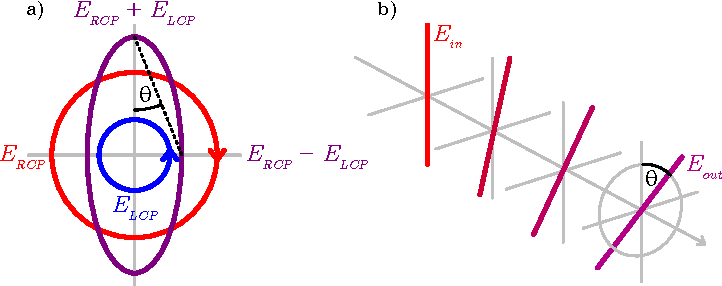
\includegraphics[scale=1.0]{./figures/background/chiroptics/cdor.pdf}
    \caption{\label{fig:background:Chirality:cdor}\textbf{a)} Schematic diagram of circular dichroism, characterised by the ellipticity ellipticity $\theta$ defined in terms of the field amplitudes of RCP and LCP light $E_{RCP}$ and $E_{LCP}$. The ellipticity is given by equation~\ref{eq:background:Chirality:CD}. \textbf{b)} Schematic diagram of optical rotation, showing linearly polarised light rotated by an angle $\theta$ throughout propagation through an optically active medium.}
\end{figure}
In linear optics, the circular dichroism at a particular wavelength of light is quantified by the ellipticity $\theta$, as defined by equation~\ref{eq:background:Chirality:CD}, and shown schematically in figure~\ref{fig:background:Chirality:cdor}a. 
\begin{equation}\label{eq:background:Chirality:CD}
    \theta = \arctan\left( \frac{E_{RCP} - E_{LCP}}{E_{RCP} + E_{LCP}} \right)
\end{equation} 
Here, $E_{RCP}$ and $E_{LCP}$ are the amplitudes of RCP and LCP light \textit{after} interaction with the chiral material. If $\operatorname{Im}(\kappa) = 0$, light can still be absorbed by the medium, but due to mirror symmetry, RCP and LCP light will be absorbed equally, and the CD as defined in equation~\ref{eq:background:Chirality:CD} is zero. For a non-zero $\operatorname{Im}(\kappa)$, $E_{RCP}$ and $E_{RCP}$ depend on both the magnitude of $\operatorname{Im}(\kappa)$, and the propagation length through the absorbing medium. If the propagation length is known, then circular dichroism can be used as a probe for the chirality parameter $\kappa$.
Correspondingly, $\operatorname{Re}(\kappa)$ describes the differential \textit{phase velocity} for LCP and RCP light. Since linearly polarised light can be represented by a superposition of equal-amplitude LCP and RCP waves, a linearly polarised wave, of vacuum wavevector $k_z$ propagating through a medium with RCP and LCP refractive indices given by $n_+$ and $n_-$ respectively, is described by equation~\ref{eq:background:Chirality:OR}~\cite[\S 8.10]{Hecht2013}.
\begin{equation}\label{eq:background:Chirality:OR}
    \begin{split}
        \mathbf{E} = E_0 \cos(k_z (\frac{n_+ + n_-}{2})z -\omega t &) \left[ \mathbf{\hat{x}} \cos(k_z (\frac{n_+ - n_-}{2})z ) \right. \\
        & \left. + \mathbf{\hat{y}} \sin(k_z (\frac{n_+ - n_-}{2}) z)\right]
    \end{split}
\end{equation}
At any point in time throughout propagation, the RCP and LCP components are oscillating in phase and with equal amplitudes, meaning that the resultant wave remains linearly polarised. However, the orientation of the linear polarisation will rotate throughout propagation, with the rate and direction of rotation depending on the magnitude and sign of $n_+ - n_-$ respectively. This effect is the chiral counterpart to birefringence, where orthogonal \textit{linear} polarisations exhibit different phase velocities. It is thus known as ``circular birefringence''. In the case of linear birefringence, optical rotation is achieved by utilising a fixed $\lambda/2$ phase shift, and rotating the mediums fast axis relative to the incident polarisation to control the angle of rotation. Conversely, a material exhibiting circular birefringence will rotate linearly polarised light continuously during propagation, shown schematically in figure~\ref{fig:background:Chirality:cdor}b. Therefore, the resulting angle of optical rotation ($\theta$ in figure~\ref{fig:background:Chirality:cdor}b) depends on both the strength of circular birefringence, and the propagation length through the medium. Optical rotation can therefore also be used as a method to characterise the chirality parameter $\kappa$ of the material. Collectively, circular dichroism and optical rotation are referred to as ``optical activity''.

Generally, in real materials the refractive index $n$ is strongly wavelength-dependent. The wavelength-dependent refractive index $n(\lambda)$ includes contributions from the wavelength-dependent structural chirality parameter $\kappa(\lambda)$. The dependence of $n(\lambda)$ on $\kappa(\lambda)$ directly leads to wavelength-dependent CD and OR, the latter specifically known as optical rotatory dispersion (ORD). CD spectra can be measured by taking extinction spectra LCP and RCP light propagating through the material, and applying equation~\ref{eq:background:Chirality:CD} at each wavelength, where $E_{RCP}$ and $E_{RCP}$ are the amplitudes of the transmitted RCP and LCP light respectively. Similarly, ORD spectra can be obtained by propagating linearly polarised light through the medium, and detecting the intensity of transmitted light through a rotatable analysing polariser. The analyser angle transmitting maximum intensity gives the resulting angle of polarisation, which can be compared to the incident polarisation to find the angle of optical rotation. Again, this can be taken at each wavelength to construct an ORD spectrum. It is important to reiterate however, that OR and CD depend on the real and imaginary parts of the same complex refractive index $n$. CD and ORD spectra are thus intrinsically linked by the Kramers-Kronig transforms: each can be obtained from the other, and they fundamentally contain the same information. 


\subsection{Chiroptical Effects from Extrinsic Chirality}\label{sec:background:Chirality:extrinsic}
It is possible to obtain a chiroptical response from structures that exhibit neither 3D nor planar chirality. Instead, chirality is introduced by the geometry of the experiment itself; the wave-vector, the surface normal and the direction of curvature on the structure form a chiral triad. 
The fundamental mechanism for this optical activity is shown in figure~\ref{fig:background:Chirality:extrinsic}. When illuminated at normal incidence, the structure geometry remains unchanged when projected onto the transverse plane of the incident light (figure~\ref{fig:background:Chirality:extrinsic} left). However, when the sample is illuminated at an oblique angle the projection of the structure geometry onto the transverse plane of incident light becomes distorted. Under inversion, the structure's projection can no longer be superimposed onto itself by in-plane rotation, and is therefore planar chiral, as shown in figure~\ref{fig:background:Chirality:extrinsic} (right). 
If optical activity due to extrinsic chirality is measured at an oblique angle of incidence $\phi$, then the chiroptical response should change sign when measured at an angle of incidence of $-\phi$. That is, any measured circular dichroism will reverse sign, and any optical rotation will rotate in the opposite direction. This can perhaps be more intuitively understood by considering the geometry shown in figure~\ref{fig:background:Chirality:extrinsic}. The projection of the structure's mirror image at oblique incidence is identical to its own projection at the opposite angle of incidence. By reversing the angle of incidence, the chirality of the experimental geometry is reversed, and any chiroptical effects will correspondingly change sign.
\begin{figure}[htb!]
    \centering
    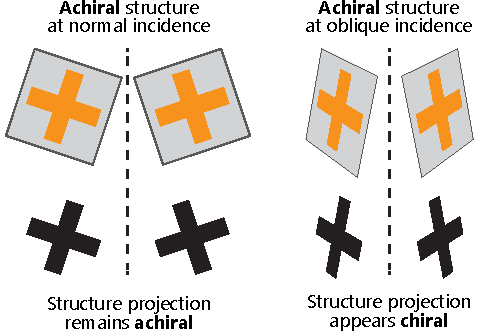
\includegraphics[scale=1.0]{./figures/background/chiroptics/extrinsic_chirality.pdf}
    \caption{\label{fig:background:Chirality:extrinsic}Schematic representation of extrinsic chirality in an achiral structure.}
\end{figure}
Plum et al. showed that asymmetric transmission (circular difference) can occur in any structure whose projection onto the transverse plane of incident light is 2-dimensionally chiral and anisotropic~\cite{Plum2011}. It is therefore possible to achieve chiroptical effects utilising geometrically simpler structures than those that are intrinsically chiral.

For applications requiring manipulation of light polarisation, such as optical rotation or circular dichroism, it is perfectly possible to use extrinsic instead of intrinsic chirality. An early study by Plum et al., for example, measured a chiroptical response from achiral split-ring structures at microwave wavelengths~\cite{Plum2009c}. These structures were shown to exhibit both circular dichroism and optical rotation when illuminated at oblique incidence. At normal incidence, no significant optical activity was measured for either structure. The circular birefringence resulted in rotation of linear polarisation exceeding $\SI{60}{\degree}$ for microwaves. Later observations, directly comparing extrinsic and intrinsic chirality, confirmed that the former can yield significantly stronger response~\cite{Maoz2012a}. 
More recent work has pushed towards optical-wavelength chiroptical responses due to extrinsic chirality.
Cao et al. demonstrated, experimentally and computationally, strong circular dichroism in the mid-IR region ($\approx\SI{2.4}{\micro\m}$), resulting from extrinsic chirality in achiral metallic nanostructures~\cite{Cao2014}. Both enantiomorphs of the structure can be obtained by tilting the sample to opposite angles. This fact, it is suggested, can be utilised to simplify experiments requiring both enantiomers of a nanostructure, by removing the need to fabricate two separate structures.
More recently, Belardini et al. have demonstrated strong chiroptical effects at \textit{optical} wavelengths from a surface of tilted nanowires~\cite{Belardini2016}. It was shown that upon rotating the sample by $\SI{180}{\degree}$, both the circular dichroism and angle of optical rotation change sign, as expected for extrinsic chirality. 
The same work also reported that extrinsic chirality affects nonlinear chiroptical measurements (discussed further in section~\ref{sec:background:NonlinearOptics}) in a similar way. Nonlinear chiroptical measurements were taken as a function of the angle of incidence of light, for opposite orientations of the nanowires. As expected, the opposite orientations resulted in a reversal of the nonlinear chiroptical response. Additional work demonstrated the same dependency of the nonlinear chiroptical response on the angle of optical incidence, and that extrinsic chirality is induced by the relative angle between the light and the surface normal~\cite{Belardini2015}.

The relative simplicity of fabrication for achiral nanostructures could open the field to more readily available and easier to mass-produce geometries. The key here would be to consider the experimental geometry as a whole. However, in experiments aiming to characterise the chirality of materials at oblique incidence, contributions to measurable chiroptical effects from extrinsic chirality can complicate analysis. Importantly, extrinsic chirality can be identified by comparing the symmetry of contributions from intrinsic and extrinsic chirality. Chiroptical effects originating from true intrinsic chirality should be invariant upon rotation of the angle of incidence. Conversely, contributions originating from extrinsic chirality will reverse as the angle of incidence changes sign.


\subsection{Chiroptical Effects from Anisotropy}\label{sec:background:Chirality:anisotropy}

It was shown earlier in section~\ref{sec:background:Chirality} that the rotation and circularly polarisation of linearly polarised light can occur in achiral, anisotropic materials.
Despite applications in polarisation optics, structural anisotropy raises issues when characterising chiral systems. 
Within stereochemistry, chiroptical analysis historically tends to occur in isotropic, homogenous liquid molecular systems~\cite{Berova2012a}. In these cases, the anisotropy of individual molecules has no significant effect on the macroscopically measured optical activity. This is due to the 3-dimensional averaging out of anisotropy for a large number of randomly oriented molecules. 
However, the work in this thesis makes use of planar metallic ``nanomaterials'', discussed in greater depth in section~\ref{sec:background:Plasmonics}. These nanomaterials are commonly fabricated by patterning metallic inclusions onto a 2-dimensional surface, and so typically cannot be isotropically arranged. 

Previous work has demonstrated that, towards the nanoscale, achiral, anisotropic structures can locally generate circularly polarised light~\cite{Hashiyada2018}. Conversely, a linearly birefringent material can convert circularly polarised light to linearly polarised light. 
Such birefringent materials can also exhibit linear dichroism (a difference in the absorption of orthogonal linearly polarisations). This can lead to an apparent circular dichroism, actually the combined effect of linear birefringence and linear dichroism. Likewise, the operation of half-wave plates demonstrates the ability for anisotropic, achiral media to result in significant optical rotation of linearly polarised light. 
When characterising the chirality of anisotropic structures, there is thus a prevailing need for experimental techniques capable of disentangling contributions from anisotropy and intrinsic chirality. 
Fortunately, chiroptical contributions from anisotropy can also be identified with symmetry considerations. Any chiroptical effects measured due to an isotropic structure's intrinsic chirality will be invariant under structure rotation. Conversely, chiroptical effects originating exclusively from anisotropy will necessarily vary as the structure is rotated, reversing sign upon $\SI{90}{\degree}$ rotation normal to the fast and slow axis of the material. However, this periodic sign change is not strictly necessary in structures that exhibit both intrinsic or extrinsic chirality \textit{and} structural anisotropy. In these cases, the two contributions are effectively competing, and complex chiroptical behaviour can emerge~\cite{Hooper2017}. Isolating the structural chirality from anisotropy and extrinsic chirality is therefore challenging, especially in planar nanomaterials which are often highly anisotropic. In sections~\ref{sec:results:OAinPlanarNanohelices} and~\ref{sec:results:HRS} two methods of experimentally isolating the intrinsic chirality of metallic nanomaterials are explored.


\section{Optical Chirality and ``Superchiral'' Light}\label{sec:background:Chirality:opticalchirality}
The interaction between a chiral molecule and a chiral electromagnetic field is expected to exhibit a dissymmetry, in that each ``handedness'' of a chiral field should interact differently with a chiral molecule or nanostructure. A field with a shorter chiral pitch, the distance over which the polarisation vector completes a $\SI{360}{\degree}$ twist, will exhibit a stronger interaction dissymmetry than a less twisted field. It had long been thought that the maximum possible chiral dissymmetry is obtained for a perfectly circularly polarised monochromatic field, however in 2010 Tang and Cohen proposed a setup in which the dissymmetry exceeds that of CPL (referred to as ``superchiral light'') at the nodes of a chiral standing wave.~\cite{Tang2010}
The strength of the field chirality can be quantified by Lipkin's 00-zilch density~\cite{Lipkin1964} referred to by Tang and Cohen as the ``optical chirality'' $C$ as defined in equation~\ref{eq:background:chirality:opticalchirality}. This quantity is a time-even pseudo-scalar, as would be expected for a measure of true chirality.
\begin{equation} \label{eq:background:chirality:opticalchirality}
    \begin{split}
        C = &\frac{\varepsilon_0 }{2}{\bf{\tilde E}} \cdot (\nabla  \times {\bf{\tilde E}}) + \frac{1}{{2\mu _0}}{\bf{\tilde B}} \cdot (\nabla  \times {\bf{\tilde B}}) \\
        = &- \frac{{{\varepsilon _0}\omega }}{2} \operatorname{Im}[ \bf{\tilde E}(\bf{r}) \cdot \bf{\tilde B}(\bf{r}) ]
    \end{split}
\end{equation}
Here, $\bf{\tilde E}$ and $\bf{\tilde B}$ denote the complex electric and magnetic field amplitudes respectively. This quantity describes the angular momentum of the curl of the optical field~\cite{Cameron2012a} and is a conserved property of the field. Tang and Cohen showed that the enantioselectivity of optical excitation of a molecule is highly dependent on $C$, and so it stands that such a superchiral field can lead to significant enhancement of the enantioselective excitation of chiral molecules.

The general microscopic response of a chiral molecule to a monochromatic electromagnetic field is described by an induced electric dipole moment $\mathbf{\tilde p}$ and magnetic dipole moment $\mathbf{\tilde m}$ as in equation~\ref{eq:background:chirality:tangDipole}.
\begin{equation}
    \label{eq:background:chirality:tangDipole}
    \begin{split}
        &{\bf{\tilde p}} = {{\tilde \alpha }_{ee}}{\bf{\tilde E}} - i{{\tilde \alpha }_{em}}{\bf{\tilde B}} \\
        &{\bf{\tilde m}} = i{{\tilde \alpha }_{em}}{\bf{\tilde E}} + {{\tilde \alpha }_{mm}}{\bf{\tilde B}}
    \end{split}
\end{equation}
Here, $\tilde{\alpha}_{ee}$ and $\tilde{\alpha}_{mm}$ correspond to $\tilde{\alpha}$ and $\tilde{\chi}$ in references~\cite{Tang2010} and~\cite{Choi2012}, 
$\alpha_{ee}$ is the electric polarisability, and $\alpha_{mm}$ is the magnetic susceptibility. $\tilde{\alpha}_{em}$ is the mixed magneto-electric polarisability and is directly related to the material chirality parameter $\kappa$ (section~\ref{sec:background:Chirality:Structural}).
Physical quantities are obtained from the real parts of equation (14). For an incident electric field $\mathbf{\tilde{E}}=\mathbf{\tilde{E}}_{0}{e}^{-i\omega t}$ and $\mathbf{\tilde{B}}=\mathbf{\tilde{B}}_{0}{e}^{-i\omega t}$ the rate of excitation of a molecule from right ($+$) and left ($-$) CPL is given by equation~\ref{eq:background:chirality:Aplusminus} \cite{Tang2010, Choi2012}.

\begin{equation} \label{eq:background:chirality:Aplusminus}
    {A^ \pm } = 
    \frac{\omega }{2}{\left\langle {{\bf{E}} \cdot {\bf{\dot p}} + {\bf{B}} \cdot {\bf{\dot m}}} \right\rangle _t} = 
    \frac{\omega }{2}{\mathop{\rm Im}\nolimits} ({{\bf{\tilde E}}^ * } \cdot {\bf{\tilde p}} + {{\bf{\tilde B}}^ * } \cdot {\bf{\tilde m}})
\end{equation}
Substituting equation~\ref{eq:background:chirality:tangDipole} into equation~\ref{eq:background:chirality:Aplusminus} leads to equation~\ref{eq:background:chirality:AplusminusFull}, which can be rewritten in terms of the generalised optical chirality $C$ to give equation~\ref{eq:background:chirality:AplusminusC}~\cite{Choi2012}. Here ${\tilde \alpha }_{em}''=\operatorname{Im}({\tilde \alpha }_{em})$.
\begin{equation} \label{eq:background:chirality:AplusminusFull}
    {A^ \pm } = \frac{\omega }{2}({\tilde \alpha ''_{ee}}{\left| {{\bf{\tilde E}}} \right|^2} + {\tilde \alpha ''_{mm}}{\left| {{\bf{\tilde B}}} \right|^2}) \pm {\tilde \alpha }_{em}''\omega {\mathop{\rm Im}\nolimits} ({{\bf{\tilde E}}^ * } \cdot {\bf{\tilde B}})
\end{equation}
\begin{equation} \label{eq:background:chirality:AplusminusC}
    {A^ \pm } \simeq \frac{\omega }{2}({\tilde \alpha ''_{ee}}{\left| {{\bf{\tilde E}}} \right|^2} + {\tilde \alpha ''_{mm}}{\left| {{\bf{\tilde B}}} \right|^2}) \pm {\tilde \alpha }_{em}''\frac{2}{\varepsilon }C
\end{equation}
The time averaged electric and magnetic energy densities ${{\left\langle {{U}_{E}} \right\rangle }_{t}}=\tfrac{\varepsilon }{4}{{\left| {\mathbf{\tilde{E}}} \right|}^{2}}$ and ${{\left\langle {{U}_{B}} \right\rangle }_{t}}=\tfrac{1}{4\mu }{{\left| {\mathbf{\tilde{B}}} \right|}^{2}}$  can be introduced here, and substituted into equation~\ref{eq:background:chirality:AplusminusC} to give the rate of excitation in terms of energy density as in equation~\ref{eq:background:chirality:AplusminusU}. 
\begin{equation}\label{eq:background:chirality:AplusminusU}
    \begin{split}
        & {A^ \pm } \simeq \frac{2}{\varepsilon }{{\tilde \alpha ''}_{ee}}\omega \left( {{{\left\langle {{U_E}} \right\rangle }_t} + \gamma {{\left\langle {{U_B}} \right\rangle }_t}} \right) \pm {\tilde \alpha }_{em}''\frac{2}{\varepsilon }C \\
        & \gamma  = \frac{{{{\tilde \alpha ''}_{mm}}}}{{{{\tilde \alpha ''}_{ee}}}}\varepsilon \mu  = \frac{{{{\tilde \alpha ''}_{mm}}}}{{{{\tilde \alpha ''}_{ee}}}}\frac{{{n^2}}}{{{c^2}}}
    \end{split}
\end{equation}
We can now define the dissymmetry factor $g$ of the chiroptical interaction by equation~\ref{eq:background:chirality:dissymmetryA}.
\begin{equation}\label{eq:background:chirality:dissymmetryA}
    g = \frac{{{A^ + } - {A^ - }}}{\frac{1}{2}({A^ + } + {A^ - })}
\end{equation}
In Tang and Cohen's proposal~\cite{Tang2010} the magnetic field was disregarded as negligible. Under this assumption, the dissymmetry factor is found to be 
\begin{equation}\label{eq:background:chirality:dissymmetryG}
    g =  - \frac{{{\tilde \alpha }_{em}''}}{{\tilde \alpha ''}_{ee}}\frac{{2C}}{{\omega {{\left\langle {{U_E}} \right\rangle }_t}}}
\end{equation}
Note that under this approximation, the dissymmetry factor splits into properties of the molecule only (${{\tilde \alpha }_{em}''}/{{\alpha }''}_{ee}$) and properties of the field only (${2C}/{\omega {{\left\langle {{U}_{E}} \right\rangle }_{t}}}$), however in the general case the dissymmetry factor cannot be separated in this way and is significantly more complex~\cite{Choi2012}.
The full expression accounting for magnetic energy density can be simplified by assuming a small dissymmetry factor such that $n_{+} \approx n_{-}$, to give equation~\ref{eq:background:chirality:dissymmetryFull}.~\cite{Choi2012}
\begin{equation}\label{eq:background:chirality:dissymmetryFull}
    g =  - \frac{{\tilde \alpha ''}_{em}}{{{\tilde \alpha ''}_{ee}}}\frac{{2C}}{{\omega [{{\left\langle {{U_E}} \right\rangle }_t} + \gamma {{\left\langle {{U_B}} \right\rangle }_t}]}}
\end{equation}
The limitation in chiroptical enhancement is now clear: in regions of low electric energy density, the magnetic energy density is maximised and should not be considered negligible. The $\gamma$ term in equation~\ref{eq:background:chirality:dissymmetryFull} is then the key limiting factor for the dissymmetry enhancement. The energy density terms in the denominator can no longer be reduced to arbitrarily small values in order to continually increase chiral dissymmetry. However, the chiral dissymmetry can still be increased by reducing the total electromagnetic energy density, increasing the structural chirality parameter of the medium, and increasing optical chirality $C$ of the electromagnetic field. 

Despite these limitations, Tang and Cohen experimentally verified enhanced chiral dissymmetry using superchiral nodes on a standing wave, as previously proposed. By comparing the fluorescence emission of chiral and achiral molecular layers under left- and right-polarised superchiral standing waves, they demonstrated an $11 \times$ dissymmetry enhancement compared to circularly polarised light~\cite{Tang2011}. This experimental configuration has clear practical limitations however, in that the target sample must be positioned at, or near, a node of a standing wave. Slight positional deviations of the sample, or the partially reflecting mirror, could easily result in the sample entering an anti-node, at which the optical chirality is minimised. To alleviate this limitation, experimental configurations have been proposed that fix the positioning of the standing wave, and the sample surface. Rather than using a partially reflective mirror to generate a standing wave, periodic photonic crystal structures have been used to form Bloch waves, which can lead to superchiral nodes at fixed positions through the photonic crystal structure~\cite{Sinibaldi2014, Pellegrini2017, Pellegrini2018}. By designing the structure and angle of optical incidence such that a node of high optical chirality occurs at the termination surface of the structure, chiral fields can be formed over large surface areas, used for sensing and characterisation of molecules attached to the material surface~\cite{Sinibaldi2014, Pellegrini2017}. These superchiral Bloch waves have been used to demonstrate two orders of magnitude increase in circular dichroism signal compared to probing with circularly polarised light~\cite{Pellegrini2017}.
Typically however, a more common method of experimentally realising superchiral light is the use of plasmonic nanomaterials, capable of generating periodic small regions of high optical chirality at the surface of a quasi-2-dimensional material. This is discussed further in section~\ref{sec:background:Plasmonics:superchiral}.


\section{Conclusions}

Across a wide range of research fields, chirality, the lack of mirror symmetry, is a key structural property, especially prevalent in biomolecular systems. Particularly, many pharmaceutical drugs are chiral, with enantiomers often exhibiting dramatically different medical effects.
Because of this, chiral optical (chiroptical) effects have become a widespread method for characterising the structural properties of complex molecular systems.
We have shown that structural anisotropy can be utilised to form chiral polarisation states of light, which can in turn be used to directly probe material chirality.
By considering the propagation of light through a medium exhibiting coupling between induced electric and magnetic dipoles, we have shown that left- and right-circularly polarised light will propagate through a chiral medium with different refractive indices. This chiral dissymmetry directly leads to circular dichroism, and optical rotation, two measurable probes of the real and imaginary parts of the chiral medium's refractive index.
In section~\ref{sec:background:Chirality:opticalchirality}, it was shown that, perhaps contrary to intuition, pure circularly polarised light does not necessarily lead to the strongest chiral dissymmetry. In fact, by interfering circularly polarised fields, the nodes of an elliptically polarised standing wave can exhibit a twisted field gradient stronger than that of CPL. This has allowed for molecular chiroptical measurements with significantly greater sensitivity than those undertaken with pure circularly polarised light.
As well as ``superchiral'' configurations, enhanced chiroptical sensitivity has been demonstrated by making use of nonlinear optics; an extremely symmetry-sensitive frequency conversion effect within media driven by intense electromagnetic fields. The following section discusses the microscopic origin of nonlinear emission, the macroscopic descriptions of nonlinear media, and the symmetry properties of second-harmonic generation in particular, for use in chiroptical characterisation measurements.
\chapter{Nonlinear Optics}\label{sec:background:NonlinearOptics}

\section{The Lorentz Oscillator}\label{sec:background:NonlinearOptics:lorentz}
In the Lorentz model of an oscillating dipole driven by an electric field $E(t)$, the 1-dimensional motion of an electron, with an effective mass $m_0$ and charge $q$, in a harmonic potential $U(x) = (1/2)kx^{2}$ is described by
\begin{equation}\label{eq:NonlinearOptics:eqMotion}
	m_{0} \frac{d^2 x}{dt^2} + m_{0} \gamma \frac{dx}{dt} + m_{0} \omega_{0}^2 x = -q E(t)
\end{equation}
Here, $x$ is the positional displacement of the electron, and $m_{0} \gamma \frac{dx}{dt}$ describes a damping force. $\omega_{0}$ describes the resonant frequency of the system, and is defined in terms of a spring constant $k$ by $\omega_{0} = \sqrt{k/m_{0}}$. The restoring force $m_{0} \omega_{0}^2 x = kx$ relates to the potential $U(x)$ by
\begin{equation}
	F_{restoring} = \frac{d}{dx} U(x) = \frac{d}{dx} (1/2)kx^{2} = kx
\end{equation}
The displacement of the electric $x(t)$ results in a dipole moment $p(t) = ex(t)$, leading to a macroscopic induced polarization of a material given by $P(t) = Np(t)$ where $N$ is the number of oscillators per unit volume.

In the case of a driving field $E(t) = E_0 e^{-(i\omega t + \phi_E)}$, oscillating at a frequency $\omega$ with a phase $\phi_E$, solutions for $x(t)$ will take the form of $x(t) = x_0 e^{-(i\omega t + \phi_x)}$. By including phase information by making $x_0$ and $E_0$ complex, these expressions can be substituted into equation~\ref{eq:NonlinearOptics:eqMotion} and solved for $x_0$ giving
\begin{equation}\label{eq:NonlinearOptics:x0}
	x_0 = \frac{-q E_0}{m_0 (\omega_{0}^2 -\omega^2 -i \gamma \omega)}
\end{equation}
The macroscopic induced polarization $P(t) = N q x(t)$ is now given by
\begin{equation}\label{eq:NonlinearOptics:PfullLinear}
	\begin{split}
		P(t) = & N q \left( \frac{-q E_0}{m_0 (\omega_{0}^2 -\omega^2 -i \gamma \omega)} \right) e^{-(i\omega t)} \\
		= & \frac{N q^2}{m_0} \left( \frac{1}{\omega_{0}^2 -\omega^2 -i \gamma \omega} \right) E_0 e^{-(i\omega t)} \\
		= & \frac{N q^2}{m_0} \left( \frac{1}{\omega_{0}^2 -\omega^2 -i \gamma \omega} \right) E(t)
	\end{split}
\end{equation}
We can now introduce the electric susceptibility $\chi$, such that the induced polarization $P(t) = \varepsilon_0 \chi E(t)$. In the simple linear case given in equation~\ref{eq:NonlinearOptics:PfullLinear}, the susceptibility is given by
\begin{equation}\label{eq:NonlinearOptics:chiFullLinear}
		\chi = \frac{N q^2}{\varepsilon_0 m_0} \left( \frac{1}{\omega_{0}^2 -\omega^2 -i \gamma \omega} \right)
\end{equation}
In the frequency domain, when driving at a frequency $\omega$ this notation can be equivalently given as $P(\omega) = \varepsilon_0 \chi(\omega) E(\omega)$.

\subsection{Nonlinear Terms}
A more general anharmonic potential contains higher order terms, and can be described by $U(x) = (1/2)kx^{2} + (1/3)\beta_2 x^3 + (1/4)\beta_3 x^4 + ...$. The corresponding restoring force leads to an equation of motion
\begin{equation}\label{eq:NonlinearOptics:eqMotionNonlinear}
	\frac{d^2 x}{dt^2} + \gamma \frac{dx}{dt} + \omega_{0}^2 x + \beta_2 x^2 +  \beta_3 x^3 + ... = -\frac{q}{m_{0} } E(t)
\end{equation}
For an oscillating $E(t)$, solving for $x(t)$ is difficult, however we can make use of the fact that, in general, $\omega_{0}^2 \ll \beta_2 \ll \beta_3 \ll ...$ to find a power series solution. By expanding $x = x_1 + x_2 + ...$ and equating successive higher orders, we obtain~\cite[\S 1.4.1]{Boyd2008a}
\begin{equation}\label{eq:NonlinearOptics:xorders}
	\begin{split}
		& \frac{d^2 x_1}{dt^2} + \gamma \frac{dx_1}{dt} + \omega_{0}^2 x_1 = -\frac{q}{m_{0} } E(t) \\
		& \frac{d^2 x_2}{dt^2} + \gamma \frac{dx_2}{dt} + \omega_{0}^2 x_2 = \beta_2 x_1^2 \\
		& \frac{d^2 x_3}{dt^2} + \gamma \frac{dx_3}{dt} + \omega_{0}^2 x_3 = 2\beta_2 x_1 x_2 + \beta_3 x_1^3 \\
		& ...
	\end{split}
\end{equation}
For convenience we here introduce the denominator function $D(\omega)$, and again consider a system driven by an electric field oscillating at a frequency $\omega$.
\begin{equation}
	D(\omega) = \omega_{0}^2 -\omega^2 -i \gamma \omega
\end{equation}
The lowest order in equation~\ref{eq:NonlinearOptics:xorders} ($x_{1}$) is equivalent to the system described by equation~\ref{eq:NonlinearOptics:eqMotion}, and so equation~\ref{eq:NonlinearOptics:x0} provides an expression for our $x_1$ term. This can be given in terms of the denominator function as
\begin{equation}
	x_{1}(t) = \frac{-q}{m_0 D(\omega)} E_0 e^{-i\omega t}
\end{equation}
Squaring $x_{1}(t)$, to obtain $x_{2}(t)$, gives both a DC component ($\omega=0$), and components oscillating at $\pm 2\omega$, proportional in amplitude to $E_{0}^2$, described by
\begin{equation}
	x_{2}(t)\vert_{\mp 2\omega} = \frac{\beta_2 q^2}{m_{0}^2 D(\pm 2\omega) D^{2}(\omega)} E_0^2 e^{\pm i 2\omega t}
\end{equation}
This is a specific degenerate case of second-order nonlinearity, where the driving field oscillates at a single frequency $\omega$. More generally, second-order nonlinear effects can be driven by two fields oscillating at different frequencies $\omega_1$ and $\omega_2$, with complex amplitudes $E_{\omega_1}$ and  $E_{\omega_2}$ respectively. In this case, $x_{2}(t)$ has components oscillating at $\omega_1 \pm \omega_2$ described by equation~\ref{eq:NonlinearOptics:x2SFG}~\cite[\S 1.4.1]{Boyd2008a}.
\begin{equation}\label{eq:NonlinearOptics:x2SFG}
	x_{2}(t)\vert_{\omega_1 \pm \omega_2} = \frac{\beta_2 q^2}{m_{0}^2 D(\omega_1 \pm \omega_2) D(\omega_1) D(\pm\omega_2)} E_{\omega_1} E_{\omega_2} e^{i (\omega_1 \pm \omega_2) t}
\end{equation}
In this work, however, we will focus on the degenerate case of second-order nonlinearity, resulting in motion at $2\omega$.

Following from equation~\ref{eq:NonlinearOptics:PfullLinear}, from  the second-order nonlinear term $x_{2}(t)$ results in an additional component in the induced polarization, $P(t)\vert_{\mp 2\omega} = N q x_{2}(t)\vert_{\mp 2\omega}$, oscillating at $2\omega$ and proportional to $E_0^2$. The second-order electric susceptibility $\chi^{(2)}$ is introduced to describe the second-order polarization, such that $P(2\omega) = \varepsilon_0 \chi^{(2)} E(\omega)^2$. Higher order nonlinearity is described by additional components in the induced polarization, characterized by higher order susceptibilities $\chi^{(n)}$.

\section{The Dielectric Susceptibility}\label{sec:background:NonlinearOptics:susceptibility}

The general, 3-dimensional, macroscopic response of a material to an electric field is described by susceptibility tensors, as shown in equation~\ref{eq:background:NonlinearOptics:susceptibility:Pti}.
\begin{equation}\label{eq:background:NonlinearOptics:susceptibility:Pti}
	P_{i}(t) =  \epsilon_{0}\big[
				\chi^{(1)}_{ij}  E_{j}(t) +
				\chi^{(2)}_{ijk}  E_{j}(t) E_{k}(t) +
				\chi^{(3)}_{ijkl}  E_{j}(t) E_{k}(t) E_{l}(t)+ \ldots
				\big]
\end{equation}
Here each of the indices $i,j,k,l,\ldots$ are the Cartesian coordinates of the associated field (ie. each index can take on $x$, $y$, or $z$.) We see that for each higher order term, an additional field is required, and the rank of the associated susceptibility tensor increases accordingly. We also find that even harmonics require a material lacking inversion symmetry. Under inversion we apply $\mathbf{r}\rightarrow -\mathbf{r}$, hence $\mathbf{P} \rightarrow -\mathbf{P}$, and $\mathbf{E} \rightarrow -\mathbf{E}$. For a centrosymmetric medium,  $\mathbf{P}(-\mathbf{E}) = -\mathbf{P}(\mathbf{E})$, and so by equating components, for any even $n$ terms, $\chi^{(n)}=-\chi^{(n)}$ meaning $\chi^{(n)} = 0$. Therefore, emission at even-order harmonics is forbidden in centrosymmetric media.

\subsection{Linear Electric Dipoles}\label{sec:background:NonlinearOptics:linearP}
The 3-dimensional linear response of a material in the dipole approximation can be described entirely by the first-order term in equation~\ref{eq:background:NonlinearOptics:susceptibility:Pti}. In the frequency domain, this becomes

\begin{equation}
	P_{i}(\omega) =  \epsilon_{0}
				\chi^{(1)}_{ij}(\omega)  E_{j}(\omega)
\end{equation}
In vector notation, this is given explicitly by
\begin{equation}
	\mathbf{P}(\omega) =  \epsilon_{0}
				\begin{bmatrix}
		\chi_{xx} & \chi_{xy} & \chi_{xz}\\ 
		\chi_{yx} & \chi_{yy} & \chi_{yz}\\ 
		\chi_{zx} & \chi_{xy} & \chi_{zz}
	\end{bmatrix} \cdot \mathbf{E}_{1}(\omega)
\end{equation}
When studying nonlinear effects, the emitted radiation from the linear response will still be present, and almost always significantly stronger than the nonlinear response.


\subsection{Second-Order Electric Dipoles}\label{sec:background:NonlinearOptics:shgP}
For second order effects $\chi^{(2)}_{ijk}$ is a rank 3 tensor of 27 components, which can be fully represented as
\begin{equation}\label{eq:background:NonlinearOptics:shgP:chiFull}
	\chi^{(2)}_{ijk} =
	\begin{bmatrix}
		\chi_{xxx} & \chi_{xyy} & \chi_{xzz} & \chi_{xyz} & \chi_{xzy} & \chi_{xzx} & \chi_{xxz} & \chi_{xxy} & \chi_{xyx}\\ 
		\chi_{yxx} & \chi_{yyy} & \chi_{yzz} & \chi_{yyz} & \chi_{yzy} & \chi_{yzx} & \chi_{yxz} & \chi_{yxy} & \chi_{yyx}\\ 
		\chi_{zxx} & \chi_{zyy} & \chi_{zzz} & \chi_{zyz} & \chi_{zzy} & \chi_{zzx} & \chi_{zxz} & \chi_{zxy} & \chi_{zyx}
	\end{bmatrix}
\end{equation}
Second-order nonlinear effects require two fields, however in practice these can be a single high-intensity field. We will first consider the general case allowing for two separate fields.

In the frequency domain, two input fields $E_{j}(\omega_{p} )$ and $E_{k}(\omega_{q} )$ lead to an internal polarisation $P_{i}(\omega_{p}\pm\omega_{q} )$. As seen earlier, the susceptibility must now contain information about the response to three fields (two in, one out), each in three dimensions. 

\begin{equation}\label{eq:background:NonlinearOptics:shgP:Psfg}
	P_{i}(\omega=\omega_{p}\pm\omega_{q} ) =  \epsilon_{0} \sum_{jk} \sum_{(pq)}
				\chi^{(2)}_{ijk}(\omega, \omega_{p},\omega_{q} ) 
				E_{j}(\omega_{p} ) E_{k}(\omega_{q} )
\end{equation}
The sum $\sum_{(pq)}$ is over fields who's frequencies sum to a fixed $\omega=\omega_{p}\pm\omega_{q}$. For two distinct input fields, at $\omega_{1}$ and $\omega_{2}$, $\omega_{p}$ and $\omega_{q}$ can each take one of these two values. This means that for known but different input frequencies, the polarisation can be given by equation \ref{eq:background:NonlinearOptics:shgP:Pw1w2}.
\begin{equation}\label{eq:background:NonlinearOptics:shgP:Pw1w2}
	P_{i}(\omega=\omega_{1}+\omega_{2} ) =  \epsilon_{0} \sum_{jk} \big[
				\chi^{(2)}_{ijk}(\omega, \omega_{1},\omega_{2} ) 
				E_{j}(\omega_{1} ) E_{k}(\omega_{2} ) +
				\chi^{(2)}_{ijk}(\omega, \omega_{2},\omega_{1} ) 
				E_{j}(\omega_{2} ) E_{k}(\omega_{1} )
				\big]
\end{equation}
Due to permutation symmetry, where $E_{j}(\omega_{1} )=E_{k}(\omega_{1} )$ and $E_{j}(\omega_{2} )=E_{k}(\omega_{2} )$, this reduces to equation \ref{eq:background:NonlinearOptics:shgP:Pw1w2b} \cite[eq. 1.3.15]{Boyd2008a}.
\begin{equation}\label{eq:background:NonlinearOptics:shgP:Pw1w2b}
	P_{i}(\omega=\omega_{1}+\omega_{2} ) =  \epsilon_{0} \sum_{jk}
				2 \chi^{(2)}_{ijk}(\omega, \omega_{1},\omega_{2} ) 
				E_{j}(\omega_{1} ) E_{k}(\omega_{2} )
\end{equation}

For second harmonic generation, we consider the case of a single input field, where now $\omega_{p}=\omega_{q}=\omega_{1}$, resulting in a polarisation $P_{i}(\omega=2\omega_{1} )$. In this case, the sum $\sum_{(pq)}$ collapses to a single term, and the polarisation is described by equation~\ref{eq:background:NonlinearOptics:shgP:Pw1w1}.
\begin{equation}\label{eq:background:NonlinearOptics:shgP:Pw1w1}
	P_{i}(\omega=2\omega_{1} ) =  \epsilon_{0} \sum_{jk}
				\chi^{(2)}_{ijk}(\omega, \omega_{1},\omega_{1} ) 
				E_{j}(\omega_{1} ) E_{k}(\omega_{1} )
\end{equation}


%\subsection{Reducing \texorpdfstring{$\chi^{(2)}$}{Lg} with Symmetry}\label{sec:background:NonlinearOptics:tensorsymmetry}

\subsection{Reducing \texorpdfstring{$\chi^{(2)}$}{Lg} with Permutation Symmetry}\label{sec:background:NonlinearOptics:permutation}
Since $E_{j}(\omega_{1} )$ and $E_{k}(\omega_{1} )$ are indistinguishable for a single input beam, in the case of SHG we can reduce $\chi^{(2)}_{i, j, k}$ to a $3\times6$ matrix. This is because (for j,k) $x,y$ and $y,x$ are equal, $x,z$ and $z,x$ are equal, and $z,y$ and $y,z$ are equal. We need only consider half of these terms, and terms where j=k. We define our new matrix $d_{il}$ with the replacements in table~\ref{table:jkl}.

\begin{table}[H]
\centering
\caption{}
\begin{tabular}{lllllll}
j,k: & 1,1 & 2,2 & 3,3 & 2,3 or 3,2 & 1,3 or 3,1 & 1,2 or 2,1 \\
l:   & 1   & 2   & 3   & 4          & 5          & 6          
\end{tabular}
\label{table:jkl}
\end{table}
The remaining terms are then rearranged, reducing from equation~\ref{eq:background:NonlinearOptics:shgP:chiFull} to
\begin{equation}\label{eq:background:NonlinearOptics:permutation:dil}
	d_{il}=
	\begin{pmatrix}
		\chi_{xxx} & \chi_{xyy} & \chi_{xzz} & \chi_{xyz} & \chi_{xzx} & \chi_{xyx}\\ 
		\chi_{yxx} & \chi_{yyy} & \chi_{yzz} & \chi_{yzy} & \chi_{yzx} & \chi_{yxy}\\ 
		\chi_{zxx} & \chi_{zyy} & \chi_{zzz} & \chi_{zyz} & \chi_{zxz} & \chi_{zyx}
	\end{pmatrix}
\end{equation}
Following the same reduction and rearrangement, the tensor product of the fields under permutation symmetry is also reduced, leaving the polarisation for second harmonic generation in 3 dimensions as
\begin{equation}\label{eq:background:NonlinearOptics:permutation:PshgFull}
	\begin{pmatrix}
		P_{x}\\ 
		P_{y}\\ 
		P_{z}
	\end{pmatrix} =
	\begin{pmatrix}
		\chi_{xxx} & \chi_{xyy} & \chi_{xzz} & \chi_{xyz} & \chi_{xzx} & \chi_{xyx}\\ 
		\chi_{yxx} & \chi_{yyy} & \chi_{yzz} & \chi_{yzy} & \chi_{yzx} & \chi_{yxy}\\ 
		\chi_{zxx} & \chi_{zyy} & \chi_{zzz} & \chi_{zyz} & \chi_{zxz} & \chi_{zyx}
	\end{pmatrix}
	\begin{pmatrix}
		E_{x}E_{x}\\ 
		E_{y}E_{y}\\ 
		E_{z}E_{z}\\
		2E_{y}E_{z}\\ 
		2E_{z}E_{x}\\ 
		2E_{x}E_{y}
	\end{pmatrix}
\end{equation}

\subsection{Reducing \texorpdfstring{$\chi^{(2)}$}{Lg} with Rotational Symmetry}\label{sec:background:NonlinearOptics:rotation}
he number of tensor components can also be reduced by considering rotational symmetry. If we rotate the system by an angle $\theta$ about a particular axis, we can define the new, rotated axes by applying the a set of coordinate transformations. For example, rotating in the $x-y$ plane, about the $z$ axis, applies the transformations
\begin{equation}\label{eq:background:NonlinearOptics:rotation:generalTrans}
    \begin{split}
        x \rightarrow x \cos{\theta} - y \sin{\theta} \\
        y \rightarrow x \sin{\theta} +y \cos{\theta} \\
        z \rightarrow z
    \end{split}
\end{equation}
In matrix notation, this is given by
\begin{equation}\label{eq:background:NonlinearOptics:rotation:MatrixTrans}
	\begin{pmatrix}
		x^{\prime}\\ 
		y^{\prime}\\ 
		z^{\prime}
	\end{pmatrix} =
	\begin{bmatrix}
		\cos{\theta} & -\sin{\theta} & 0\\ 
		\sin{\theta} & \cos{\theta} & 0\\ 
		0 & 0 & 1
	\end{bmatrix}
	\begin{pmatrix}
		x\\ 
		y\\ 
		z
	\end{pmatrix}
\end{equation}
Following the same reasoning, we reach the matrices for rotating about each coordinate axis.
\begin{equation}\label{eq:background:NonlinearOptics:rotation:AllRotationMatrices}
\begin{split}
	&R(\theta_{z})_{ij} =
	\begin{bmatrix}
		\cos{\theta_{z}} & -\sin{\theta_{z}} & 0\\ 
		\sin{\theta_{z}} & \cos{\theta_{z}} & 0\\ 
		0 & 0 & 1
	\end{bmatrix}\\	
	&R(\theta_{y})_{ij} =
	\begin{bmatrix}
		\cos{\theta_{y}} & 0 & \sin{\theta_{y}}\\ 
		0 & 1 & 0\\ 
		-\sin{\theta_{y}} & 0 & \cos{\theta_{y}}
	\end{bmatrix}\\	
	&R(\theta_{x})_{ij} =
	\begin{bmatrix}
		1 & 0 & 0\\ 
		0 & \cos{\theta_{x}} & -\sin{\theta_{x}}\\ 
		0 & \sin{\theta_{x}} & \cos{\theta_{x}}
	\end{bmatrix}\\	
\end{split}
\end{equation}
Rotations around multiple axes can then be solved by applying successive rotation matrices in the same way. 

For rotational symmetry in the $x-y$ plane, we first rotate the tensor by the angle corresponding to our symmetry using
\begin{equation}\label{eq:background:NonlinearOptics:rotation:RotateChi}
	\chi_{ijk}^{\prime} =  R(\theta)_{i\alpha}R(\theta)_{j\beta}R(\theta)_{k\gamma}\chi^{(2)}_{\alpha \beta \gamma}
\end{equation}
Due to symmetry, the tensor should remain unchanged under this transformation, and so we impose the equality $\chi_{ijk}^{\prime}=\chi_{ijk}$ to find any component dependencies. Solving for rotational symmetry can show various tensor components as being dependant, or necessarily equalling zero. Examples of this are given in Appendix~\ref{sec:appendix:rotations}.


\paragraph{C\texorpdfstring{$_4$}{Lg} Symmetry and Rotational Isotropy} \label{sec:appendix:RotIso}
It is worth making note of the special case of planar 4-fold rotational symmetry (C$_4$ symmetry in Schoenflies notation), whose tensor and dependencies are found in Appendix~\ref{sec:appendix:rotations:4foldRot}. Due to the set of dependencies and vanishing components, applying an arbitrary $x-y$ rotation to the C$_4$ tensor results in no change of any components. 

Furthermore, a structure is isotropic (C$_{\infty}$ in Schoenflies notation) when the tensor remains unchanged under any rotation. In tensor notation, for any value of $\theta$ we can say that in an isotropic structure
\begin{equation}\label{eq:background:NonlinearOptics:rotation:RotIsoTensor}
	R(\theta_{z})_{i\alpha}R(\theta_{z})_{j\beta}R(\theta_{z})_{k\gamma}\chi^{(2)}_{\alpha \beta \gamma}
	=\chi^{(2)}_{ijk}
\end{equation}
Since this condition is met for a  C$_4$ tensor, 2-dimensional rotational isotropy is found to give the same tensor dependencies as under C$_4$ symmetry~\cite[\S E.1.8]{Popov1995}. In full, we find that for both C$_4$ and C$_{\infty}$ structures, the tensors can be reduced to
\begin{equation}\label{eq:background:NonlinearOptics:rotation:IsotropicChi}
	\chi^{(2)}_{ijk} =
	\begin{bmatrix}
		0 & 0 & 0 & \chi_{xyz} & \chi_{xzy} & \chi_{xzx} & \chi_{xxz} & 0 & 0\\ 
		0 & 0 & 0 & \chi_{yyz} & \chi_{yzy} & \chi_{yzx} & \chi_{yxz} & 0 & 0\\ 
		\chi_{zxx} & \chi_{zyy} & \chi_{zzz} & 0 & 0 & 0 & 0 & \chi_{zxy} & \chi_{zyx}
	\end{bmatrix}
\end{equation}
with dependencies given by
\begin{equation}\label{eq:background:NonlinearOptics:rotation:IsotropicDependancies}
\begin{split}
	&\chi_{xyz} = -\chi_{yxz}, \chi_{xzy} = -\chi_{yzx}, \chi_{xzx} = \chi_{yzy} \\
	&\chi_{xxz} = \chi_{yyz}, \chi_{zxx} = \chi_{zyy}, \chi_{zxy} = -\chi_{zyx} \\
	&\chi_{zzz}
\end{split}
\end{equation}



\subsection{Reducing \texorpdfstring{$\chi^{(2)}$}{Lg} with Mirror Symmetry}\label{sec:background:NonlinearOptics:mirror}
So far we have only considered structure lacking mirror symmetry, that is those which are chiral. The application of mirror symmetry for achiral structures can further reduce the number of independent tensor components.

A reflection in the $y$ axis can be described by a transformation matrix

\begin{equation}\label{eq:background:NonlinearOptics:mirror:yReflect}
	A^{y}_{ij} =
	\begin{bmatrix}
		-1 & 0 & 0\\ 
		0 & 1 & 0\\ 
		0 & 0 & 1
	\end{bmatrix}\\	
\end{equation}
If the line of mirror symmetry lies at an angle relative to this, the rotation matrices in equation~\ref{eq:background:NonlinearOptics:rotation:AllRotationMatrices} can be applied to the system first. 

Under mirror symmetry about the $y$ axis, we impose the equality
\begin{equation}\label{eq:background:NonlinearOptics:mirror:MirrorSymmetry}
	A^{y}_{i\alpha}A^{y}_{j\beta}A^{y}_{k\gamma}\chi^{(2)}_{\alpha \beta \gamma}
	=\chi^{(2)}_{ijk}
\end{equation}
From here, the initial and reflected tensors can be compared. It is found that the general tensor for such an achiral structure reduces to
\begin{equation}\label{eq:background:NonlinearOptics:mirror:chiMirrory}
	\chi^{(2)}_{ijk} =
	\begin{bmatrix}
		0 & 0 & 0 & 0 & 0 & \chi_{xzx} & \chi_{xxz} & \chi_{xxy} & \chi_{xyx}\\ 
		\chi_{yxx} & \chi_{yyy} & \chi_{yzz} & \chi_{yyz} & \chi_{yzy} & 0 & 0 & 0 & 0\\ 
		\chi_{zxx} & \chi_{zyy} & \chi_{zzz} & \chi_{zyz} & \chi_{zzy} & 0 & 0 & 0 & 0
	\end{bmatrix}
\end{equation}
These component reductions can then be applied on top of any other symmetries exhibited by the structure.

\paragraph{Chiral Isotropic Structures}
\label{sec:ChiralIso}

Another special case worth noting regards mirror symmetry in planar isotropic (and C$_4$) structures. Under mirror symmetry, the C$_4$/C$_\infty$ tensor (equation~\ref{eq:background:NonlinearOptics:rotation:IsotropicDependancies}) reduces to
\begin{equation}\label{eq:background:NonlinearOptics:mirror:IsotropicMirrorChi}
	\chi^{(2)}_{ijk} =
	\begin{bmatrix}
		0 & 0 & 0 & 0 & 0 & \chi_{xzx} & \chi_{xxz} & 0 & 0\\ 
		0 & 0 & 0 & \chi_{yyz} & \chi_{yzy} & 0 & 0 & 0 & 0\\ 
		\chi_{zxx} & \chi_{zyy} & \chi_{zzz} & 0 & 0 & 0 & 0 & 0 & 0
	\end{bmatrix}
\end{equation}
Since only 3 independent components are removed, the chirality of an isotropic structure can be fully described by the following components:
\begin{equation}\label{eq:background:NonlinearOptics:mirror:IsoChiralComponents}
\chi_{xyz} = -\chi_{yxz}, \chi_{xzy} = -\chi_{yzx}, \chi_{zxy} = -\chi_{zyx} 
\end{equation}
In the case of SHG, applying permutation symmetry reduces this further to
\begin{equation}\label{eq:background:NonlinearOptics:mirror:ReducedIsoChiral}
	d_{il} = 
	\begin{pmatrix}
		0 & 0 & 0 & 0 & \chi_{xzx} & 0\\ 
		0 & 0 & 0 & \chi_{yzy} & 0 & 0\\ 
		\chi_{zxx} & \chi_{zyy} & \chi_{zzz} & 0 & 0 & 0
	\end{pmatrix} 
\end{equation}
The chirality is now described by a single independent component, since under permutation symmetry $\chi_{xyz} = -\chi_{yzx}$. Because of this, for C$_4$/C$_\infty$ structures the chiral contribution to SHG is often parametrized by this single ``chiral component''~$\chi_{xyz}$.

\section{Second-Harmonic Generation as a Probe for Chirality}\label{sec:background:NonlinearOptics:chirality}

From section~\ref{sec:background:NonlinearOptics:susceptibility} we know that non-zero SHG intrinsically requires a lack of centrosymmetry. For chiroptical measurements, this presents a clear advantage over the analysis of linear chiroptical effects. In linear measurements, any achiral background will contribute to the overall measured signal, reducing the contrast of chiroptical effects. However, an achiral bulk material cannot result in even-order nonlinear emission: SHG is forbidden, and so the achiral background is removed. In a system of chiral molecules amongst an achiral background, only the chiral structures, and weak contributions from surface interfaces, can contribute to SHG, drastically increasing the contrast in chiroptical dissymmetry.

Aside from the background-reduction advantages, a somewhat more subtle advantages is also presented: Unlike linear chiroptical effects which \textit{require} coupling between electric dipoles and, typically weak, magnetic dipoles (section~\ref{sec:background:Chirality:Structural}), we have shown in section~\ref{sec:background:NonlinearOptics:mirror} that any structure lacking mirror symmetry can have a chiral contribution to SHG within the electric dipole approximation alone. 
In second-harmonic generation experiments, analogues of linear circular dichroism and optical rotation can thus be measured. Second-harmonic generation optical rotation (SHG-OR) closely follows the definition discussed in section \ref{sec:background:Chirality:Chiroptics}: The angle of SHG-OR is given by the angle between the incident polarisation axis, and the angle of linearly polarised SHG from the material. The nonlinear analogue of circular dichroism is, however, somewhat less clearly defined. Often, SHG optical activity experiments measure a difference in the SHG \textit{intensity} from RCP and LCP incident light, $I_{RCP}$ and $I_{LCP}$ respectively. This is then normalised to $(I_{RCP} - I_{LCP})/(I_{RCP} + I_{LCP})$, and this quantity is called the SHG circular dichroism. However, this quantity typically gives no spectral information, and relates to the field intensity, rather than amplitude. A more appropriate term is ``circular intensity difference'' (CID), as used commonly in Raman optical activity measurements~\cite[\S 1.4]{Barron2004}. The CID is defined identically, and will be used here as a more suitable naming convention. The SHG-CID is thus defined by
\begin{equation}\label{eq:background:NonlinearOptics:CID}	
	\mathrm{SHG \mhyphen CID} = \frac{I_{RCP}^{SHG} - I_{LCP}^{SHG}}{I_{RCP}^{SHG} + I_{LCP}^{SHG}}
\end{equation}
Importantly, since the electric-dipole-only mechanism of the SHG chiroptical effects is fundamentally different to their linear chiroptical counterparts, SHG-CID and SHG-OR are not intrinsically linked by any simple relation. The two effects provide complementary information, allowing for more comprehensive structural characterisation.

While strong SHG optical rotation has been demonstrated in chemical characterisation applications~\cite{Byers1994, Pena2006}, it has received significantly less attention than the relatively widespread use of SHG-CD/CID. First introduced in 1993~\cite{Petralli-Mallow1993}, SHG-CD/CID was shown to be 3 orders of magnitude higher contrast than linear optical activity.
Even early experiments demonstrated monolayer sensitivity to both chirality and anisotropy when measuring SHG circular dichroism spectra~\cite{Byers1994a}, attributed to SHG-CD being an electric dipole allowed effect. Further experiments and theoretical analysis showed that since SHG-CD is electric dipole allowed, it can be much more sensitive to structural chirality than linear techniques, which require magneto-electric cross coupling, often present but not necessarily found in chiral structures~\cite{Verbiest1994b}. It has, however, also been shown that magneto-electric cross coupling can still contribute to SHG circular dichroism, by measuring SHG circular and linear dichroism in helical aggregates of achiral molecules~\cite{Fujiwara2004}.
In more recent years, nonlinear chiroptical measurements have been combined with spectroscopic and microscopic measurement techniques. Again largely due to extreme symmetry/surface sensitivity, SHG microscopy has significant advantages over linear microscopy in many cases, in particular for cellular and tissue imaging. Samples can be pumped by intense laser light in the IR spectral region, allowing structural information to be obtained without the need for pumping in the UV, required by many fluorescence techniques, but often where the most sample damage is caused due to strong absorption in molecular systems~\cite{Campagnola2011}. SHG-CD/CID imaging has thus been used as a high-contrast chirally sensitive method for imaging and obtaining structural information of tissue samples~\cite{Lee2013a, Campbell2016}, even allowing differentiation between skin tissue with and without disorders~\cite{Chen2012}. Beyond bio-imaging and chemical characterisation, second-harmonic generation has been used in the chiroptical characterisation of metallic nanomaterials, through both nonlinear microscopy~\cite{Huttunen2011, Valev2012a, Mamonov2017} and more direct measurements~\cite{Guerrero-Martinez2011, Belardini2014, Hooper2017}. Such nanomaterials often lead to further enhancement of nonlinear emission, and are discussed further in section~\ref{sec:background:NonlinearOptics:plasmonic}. 



\section{Conclusions}

By considering the electromagnetic behaviour of a medium within the electric dipole approximation, we have shown how nonlinear optical measurements, specifically second-harmonic generation, can give robust information about the symmetry of a material.
Nonlinear counterparts to the measurable chiroptical effects described in section~\ref{sec:background:Chirality:Chiroptics} are known to be much more sensitive, and higher contrast, than linear effects, while providing complementary information. This is typically owing to the significantly reduced background from achiral contributions, and the high symmetry-sensitivity of SHG emission.
In an isotropic, chiral medium, the intrinsic chirality is described by a single independent susceptibility tensor component. However, the chirality of an anisotropic medium is described by a large number of independent components, entangled with terms associated with anisotropy. Despite this, chiroptical effects originating from structural anisotropy will have very different symmetry to those originating from intrinsic chirality. Therefore, in anisotropic structures, further consideration of the symmetry of the response can allow the disentangling of chirality from anisotropy. 
Generally, especially in molecular systems, the nonlinear response of a material is much weaker than the linear response. By fully exploiting the symmetry sensitivity of SHG, this response can be enhanced and utilised in chiroptical characterisation experiments, however in molecular systems this is often not possible. In the following chapter, we will discuss the emergence of plasmonic nanomaterials, which allow unprecedented enhancement of nonlinear emission, chiroptical dissymmetry, and allow the virtually limitless exploration of structurally-tailored artificial metamaterials.

\chapter{Plasmonic Nanomaterials}\label{sec:background:Plasmonics}

\begin{itemize}
    \item Brief literature overview of nanostructure fabrication, brief history of plasmonic nanomaterials.
    \item Recent advances in the fabrication of nano-scale, tailor-designed structures have allowed the exploration of novel optical effects arising from the interaction between light and nanomaterials. Perhaps most commonly exploited are plasmonic materials: metallic structures within a dielectric environment whose optical properties are affected not only by material choice, but also their structural geometry.
    \item Find some seminal paper about plasmonic materials
\end{itemize}
The general response of a metal surface to incident light can be modelled in terms of plasma oscillations. By treating the metal as a free-electron gas (plasma) surrounding a lattice of positive charges, the electromagnetic response can be described by the motion of this plasma in response to external electromagnetic fields. 
At a metal-dielectric interface, incident light can drive electron-density waves that propagate along the metal surface. The coupled electromagnetic radiation and electron-density waves are known as surface plasmon polaritons (SPPs), and will propagate along the metal-dielectric interface, with an exponentially decaying intensity normal to the surface. 

\begin{figure}[htb!]
    \centering
    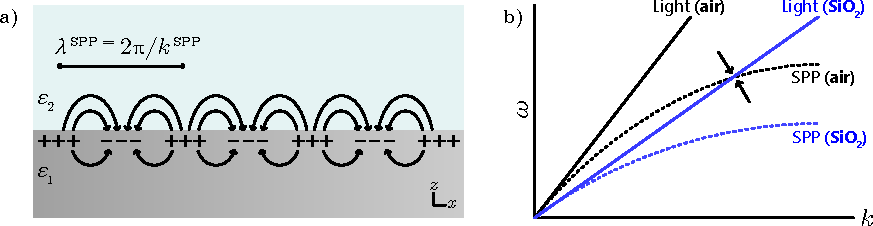
\includegraphics[scale=1.0]{./figures/background/plasmonics/spp.pdf}
    \caption{\label{fig:background:Plasmonics:SPP} \textbf{a)} Schematic of a surface plasmon polariton, of wavevector $k^{SPP}$, at a metal-dielectric interface. Charge density waves form in the metal surface, leading to surface-localised electromagnetic fields at the dielectric interface. \textbf{b)} Representative dispersion curves for surface plasmon polaritons and light at the interface of air or SiO$_2$. For any particular interface, SPPs cannot be excited by light impinging from the dielectric at that interface. Light propagating through glass can however be phase-matched to a SPP at a metal-air interface, for example. The momentum-matching point is illustrated with arrows. }
\end{figure}

We consider an interface between a metal and a dielectric, of permittivities $\varepsilon_1$ and $\varepsilon_2$ respectively (figure~\ref{fig:background:Plasmonics:SPP}a). The metal necessarily has permittivity ${\mathop{\rm Re}\nolimits}(\varepsilon_1)<0$. Excitation of SPPs require the real parts of $\varepsilon_1$ and $\varepsilon_2$ to be of opposite sign, that is, the interface is between a conductor and an insulator. In this configuration, the dispersion relation for a surface plasmon polariton propagating in the $x$ direction, oscillating at frequency $\omega$, is given by equation~\ref{eq:Plasmonics:SPPdispersion}~\cite[\S 2.2]{Maier2007}. 
\begin{equation}\label{eq:Plasmonics:SPPdispersion}
    k^{SPP}_{x} = k_0 \sqrt{\frac{\varepsilon_{1}\varepsilon_{2}}{\varepsilon_{1}+\varepsilon_{2}}} = \frac{\omega}{c} \sqrt{\frac{\varepsilon_{1}\varepsilon_{2}}{\varepsilon_{1}+\varepsilon_{2}}}
\end{equation}
For light incident on the interface via the dielectric described by $\varepsilon_2$, the optical dispersion relation $k_0 = \omega / c = \omega \sqrt{\mu_0 \varepsilon_2}$ shows that the optical momentum in the direction of SPP propagation will always be lower than that of the SPP (figure~\ref{fig:background:Plasmonics:SPP}b). Conservation of momentum must be considered when optically exciting surface plasmon polaritons, and so SPPs cannot be excited by light incident from the same dielectric as at the metal interface. Various experimental configurations have been demonstrated to allow the excitation of SPPs with optical radiation~\cite{Maier2007, Roh2011}, most commonly the Kretschmann and Otto geometries. These involve exciting a SPP at a metal-dielectric interface with light propagating through a different dielectric, interacting at an adjacent interface. In order for momentum matching to be properly realised, the projection of $k_0$ onto the axis of SPP propagation must match, and so depends strongly on the angle of optical incidence. Importantly for many applications, this angle is highly sensitive to changes in the dielectric environment. This allows the characterisation molecules attached to the metal surface by scanning the angle of incidence and observing induced shifts, leading to applications in molecular sensing and characterisation~\cite{Roh2011}.

In this work, we make use of plasmonic structure with characteristic dimensions comparable to, or smaller than, the wavelength of light in order to alleviate the momentum matching conditions. In these cases, the surface plasmons are confined to the nanoparticle surface, and are known as localised surface plasmons.


\section{Localised Surface Plasmons}\label{sec:background:Plasmonics:Metamaterials}

For small diameter $d \ll \lambda$ metallic nanoparticles, the phase of an oscillating electromagnetic field can be assumed constant over the particle, known as the ``quasi-static approximation''. In this approximation, the electron gas is driven to coherently oscillate at the particle surface. The lowest-order response of the particle to incident light can thus be described by an induced dipole moment $\bf{\tilde p}$, much like the simple Lorentz oscillator in section~\ref{sec:background:NonlinearOptics:lorentz} (figure~\ref{fig:background:Plasmonics:LSP}a).
For a metallic nanoparticle of permittivity $\varepsilon_1$ surrounded by a dielectric of permittivity $\varepsilon_2$, the induced dipole moment is described by equation~\ref{eq:Plasmonics:LSPdipole}. 
\begin{equation}\label{eq:Plasmonics:LSPdipole}
    {\bf{\tilde p}} = {\bf{\tilde \alpha }}{\bf{\tilde E}}
\end{equation}
As in section~\ref{sec:background:Chirality:opticalchirality}, $\bf{\tilde \alpha }$ describes the complex electric polarisability of the particle, and depends strongly on the nanoparticle material, geometry, and the permittivity of the surrounding medium.
Importantly, the induced dipolar plasmon mode is non-propagating, and so the momentum-matching requirements for exciting propagating surface plasmon polaritons are alleviated. The localised surface plasmon can be coherently excited by any oscillating electromagnetic field, and will reach a maximum excitation efficiency at a particular resonant frequency determined by the effective polarisability ${\tilde \alpha }(\omega)$ of the nanoparticle.
Analytical expressions for ${\tilde \alpha }(\omega)$ are well established for simple spherical nanoparticles of radius $a \ll \lambda$ and permittivity $\varepsilon(\omega)$~\cite{Maier2007, Collins2017}, given by equation~\ref{eq:Plasmonics:LSPalphaSphere}. 
\begin{equation}\label{eq:Plasmonics:LSPalphaSphere}
    {\tilde \alpha } = 4\pi a^3 \frac{\varepsilon (\omega) - \varepsilon_2 (\omega)}{\varepsilon (\omega) + 2\varepsilon_2 (\omega)}
\end{equation}
At the point where $\lvert \varepsilon (\omega) + 2\varepsilon_2 (\omega) \rvert$ is at it's minimum, i.e $\varepsilon (\omega) = -2\varepsilon_2 (\omega)$, the polarisability is maximally enhanced, determining the resonant frequency of the localised surface plasmon. However, in many systems the nanoparticle geometry is significantly more complex, and the LSP resonance cannot be determined analytically. Regardless of the particle geometry however, a particular resonant frequency will exist at which the plasmonic nanoparticle will resonantly scatter. Similar to surface plasmon polaritons, the sensitivity of the resonant frequency to the dielectric environment makes spectral analysis of the plasmonic scattering a sensitive technique for characterising nearby molecules, and has also gained popularity in molecular sensing applications~\cite{Petryayeva2011a, Polavarapu2014, Cheng2015}.

Another interesting application of deep sub-wavelength plasmonic nanostructures it the possibility of fabricating artificial ``metamaterials''. In arrays of nanoparticles supporting localised surface plasmons, the system can be modelled as an array of oscillators with effective polarisabilities. The macroscopic behaviour of the array can then be described as an effective medium, with a susceptibility describing its optical response as in section~\ref{sec:background:NonlinearOptics:susceptibility}. Now, the macroscopic optical properties of the metamaterial are strongly related to the geometry of the individual nanoparticle inclusions, offering unprecedented flexibility to design materials exhibiting optical properties never observed in nature. An often cited example of this is the possibility of a perfect optical lens formed from a metamaterial with negative refractive index, as proposed by Veselago~\cite{Veselago1968}, and later expanded on by Pendry~\cite{Pendry2000}. Further work has proposed the use of metamaterials for photonic devices such as perfect reflectors~\cite{Moitra2015}, polarisation optics~\cite{Cong2015}, and chiral-optical devices, expanded on in section~\ref{sec:background:Plasmonics:chiralPlasmonics}.


\begin{figure}[htb!]
    \centering
    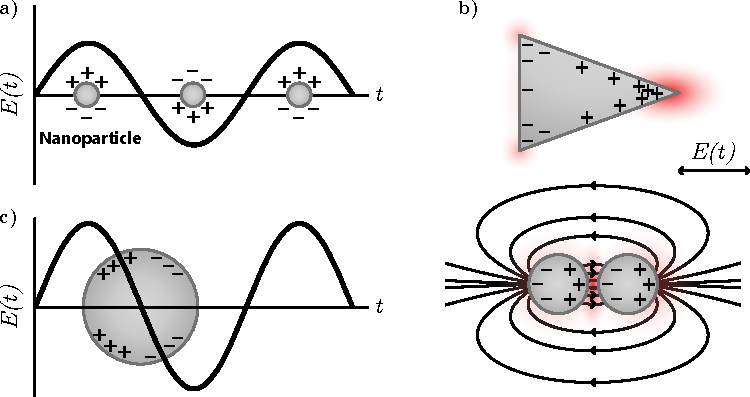
\includegraphics[scale=1.0]{./figures/background/plasmonics/lsp.pdf}
    \caption{\label{fig:background:Plasmonics:LSP} \textbf{a)} For sub-wavelength metallic nanoparticles, charge is coherently driven at the surface, and the particle can be approximated to an oscillating dipole. \textbf{b)} A pair of nanoparticles separated by some small distance will couple via the near-field, and function as a single dipole with an additional capacitance from the gap. Charge is efficiently confined to the inner surface, resulting in an enhanced electric field intensity between the two particles.}
\end{figure}


\subsection{Electromagnetic Field Confinement}\label{sec:Plasmonics:confinement}

\begin{itemize}
    \item Enhancement via localised surface plasmon resonance (excitation/scattering). 
    \begin{itemize}
        \item When a metallic nanoparticle is excited close to a plasmon resonance, the induced dipole oscillates at maximum amplitude. This results in a resonant scattering and absorption of light, leading to locally enhanced electromagnetic fields around the particle. 
        \item For sub-wavelength nanoparticles, this allows for sub-wavelength field confinement. The localised surface plasmon mode volume is limited by the particles sub-wavelength dimensions. Since the local electromagnetic field is determined by the, now tightly confined, surface plasmon mode, coupling this mode to incident light results in a confined local electromagnetic field at the particle surface.
        \item Example of enhancement from single nanoparticles
    \end{itemize}
    \item Enhancement via coupled localised surface plasmons (capacitance)
        \begin{itemize}
            \item A simple example is a pair of sub-wavelength nanoparticles, separated by a distance $d \ll \lambda$. This system behaves as a pair of point dipoles interacting via the near-field (figure~\ref{fig:background:Plasmonics:LSP}b). In the limit of small separation $d$, the coupled system will radiate as a dipole, and resonantly scatter when excited by light at it's resonant frequency. However, when driven by a field polarised along the chain axis, the gap between particles introduces a capacitance dependent on particle geometry and separation. This capacitance shifts the resonant frequency of the hybridised plasmon mode along that axis.
            \item Crucially, the capacitance of the gap results in the confinement of charge on the inner surfaces of the particles. This confinement of charge directly leads to confinement of the electromagnetic fields in the region between particles.
            \item Example of enhancement from coupled nanoparticles
        \end{itemize}
    \item Enhancement via lightning-rod effect (charge confinement)
    \begin{itemize}
        \item An additional enhancement in field confinement can come from the ``lightning-rod effect''. In the context of electrostatics, the lightning-rod effect describes the confinement of electric fields at sharp gradients of conducting structures, such as corners or tapered tips. Charge is confined more efficiently to regions of sharp surface gradients on a charged conductor, and so the electric field lines at the surface of the conductor will generally be localised around these sharp features.
        \item While not necessarily a relevant enhancement when considering coupled spherical nanoparticles, nanostructure geometries with sharper features, especially when multiple sharp features are closely coupled to each other, can greatly benefit from the additional confinement associated with the lightning-rod effect.
        \item Examples of field hotspots at the edges of nanostructures
        \begin{itemize}
            \item Direct observation of near-field localisation around the sharp features of a chiral nanostructure by ``nano-jets''~\cite{Valev2012d}
        \end{itemize}
    \end{itemize}
    
    \item Applications (literature review)
    \begin{itemize}
        \item Frequently used for SERS
        \item Sub-wavelength imaging (brief)
        \item Enhancement in chiral-optical measurements. Anything NOT about superchiral light, eg molecules between coupled spherical nanoparticles (see review sections).
        \item Enhanced nonlinear effects (due to strong intensity dependence) (most relevant to this work)
    \end{itemize}
\end{itemize}

\section{Beyond the Quasi-Static Approximation}
\begin{itemize}
    \item Intermediate regime of nanostructures, beyond the quasi-static approximation. Structure dimensions are close to, or larger than, the wavelength.
    \item The near-field optical behaviour in this regime can be understood in terms of higher order current density modes.
    \begin{itemize}
        \item The geometry of the metallic surface will permit a set of plasmon modes.
        \item Higher order plasmon modes can be excited across the surface of the structure.
        \item These modes are non-propagating standing waves, and have zero net momentum. Thus, even in this intermediate regime momentum matching is not a requirement to excite surface plasmons.
    \end{itemize}
    \item Literature review
    \begin{itemize}
        \item Zheng's work demonstrated that the plasmonic response of metallic nanostructures in this intermediate regime can be decomposed into a set of current density eigenmodes~\cite{Zheng2012}. This work was extended to collections of coupled nanostructures~\cite{Zheng2013}. 
        \item The optical response can be further understood by applying group theory to the plasmonic eigenmode set~\cite{Zheng2015}, allowing the current density modes to be grouped by the optical polarisation states that exclusively excite them.
    \end{itemize}
\end{itemize}


\section{Chiral Plasmonic Nanostructures} \label{sec:background:Plasmonics:chiralPlasmonics}
\begin{itemize}
    \item Freedom of fabrication techniques allow symmetries to be explored.
    \item Second-order nonlinear processes, which already enhance chiroptical measurements, can themselves be enhanced as described in section~\ref{sec:Plasmonics:confinement}.
    \item Literature review. Lots of references in~\cite[\S 3.2]{Collins2017}
\end{itemize}

\subsection{Superchiral Fields from Plasmonic Metasurfaces}
\begin{itemize}
    \item Literature review (directly from \cite[\S 4.3]{Collins2017})
\end{itemize}

\section{Enhanced Second-Harmonic Generation}\label{sec:background:NonlinearOptics:plasmonic}

\chapter{Enantiomorphing Chiral Nanostructures}\label{sec:results:EnantiomorphingChiralCrosses}


Sections of this chapter have been copied verbatim from the (published) manuscript \textit{``Enantiomorphing Chiral Plasmonic Nanostructures: A Counterintuitive Sign Reversal of the Nonlinear Circular Dichroism''}, Joel T. Collins et. al. \cite{Collins2018}. 
Experiments were planned by V. K. Valev. Samples were prepared by N. V. S. Braz and P. A. Warburton. SHG microscopy experiments were executed by V. K. Valev, E. Slenders and M. Ameloot. Linear scattering spectra were obtained by myself and C. Kuppe, and analysed by myself. Near-field and scattering simulations were performed by X. Zheng, G. A. E. Vandenbosch, and V. Moshchalkov. Numerical simulations of the linear far-field reflection CID were performed by S. Zu and Z. Fang. 
Analysis of the nonlinear microscopy data was performed by myself, with Python code including sections written by V. K. Valev. The formulation and analysis of modal circular-dichroism based on the near-field simulations was also performed by myself. I produced the manuscript draft on which this chapter is based.

\bigskip \noindent
In section~\ref{sec:background:Plasmonics:LSP} we discussed the formation of electric field ``hotspots'' at the surface of plasmonic nanomaterials, which can enhance both second-harmonic generation, and chiroptical interactions. These hotspots depend strongly on the optical wavelength and nanostructure geometry.
Properly understanding the properties of these chiral hotspots is crucial for their applications, for instance enhancing the optical interactions with chiral molecules. 
Here, by designing 35 intermediate geometries, a plasmonic nanostructure array is ``enantiomorphed'' from one handedness to the other, passing through an achiral geometry. 
Nonlinear multiphoton microscopy is used to demonstrate a new kind of double-bisignate circular dichroism due to enantiomorphing, rather than wavelength change.
From group theory, a fundamental origin of this plasmonic chiroptical response is then proposed. 

\section{Introduction}\label{sec:results:EnantiomorphingChiralCrosses:introduction}
Historically, chirality has been primarily associated with stereochemistry. However, while chirality can be crucial for understanding molecules, molecules are not best suited for understanding chirality. 
Ideally, we would like to be able to vary the chirality of a particular structure, i.e., to follow the chiroptical response as chiral systems transition from one form into another. While some geometric parameters of molecular systems can be varied to study chirality~\cite{Katzenelson2000}, it is not possible to \emph{freely} control arbitrary geometric properties of molecules. Modern nanofabrication techniques have gone some way to lifting this limitation.
Using modern nanofabrication, it is possible to explore a more complete evolution of chiral forms, by preparing sets of intermediate geometries. This opens the possibility to tune and optimise the chirality parameters. For instance, by maximising the geometric chirality parameter, it is possible to achieve negative refractive index materials with applications in super-lenses \cite{Khorasaninejad2016}, as well as various applications that depend on the control of circularly polarised light (CPL). 
Moreover, by optimising optical chirality (section~\ref{sec:background:Chirality:opticalchirality}), ``superchiral'' light configurations can be achieved. Importantly, optical chirality is particularly enhanced at the surface of chiral plasmonic nanostructures (section~\ref{sec:background:Plasmonics:superchiral}), resulting in large enhancements in measurable circular dichroism (CD).

Despite the advantages of creating intermediate geometries, it is rare to find studies where these have been investigated in detail. Between two enantiomorphs, there can be several pathways for intermediate geometries, illustrated in figure~\ref{fig:results:EnantiomorphingChiralCrosses:setup}a. 
Also, \textit{a priori}, it is not clear what the best number of intermediate geometries should be. This is highly dependent on the geometric and material properties of the structures, as well as on the wavelength ranges used. In literature, examples can be found of studying both enantiomorphs of a structure, its achiral variant, and a small number of intermediate steps only \cite{Zu2016}. Consequently, important and interesting behaviour can go unnoticed.

\begin{figure}[htb]	
    \centering	
    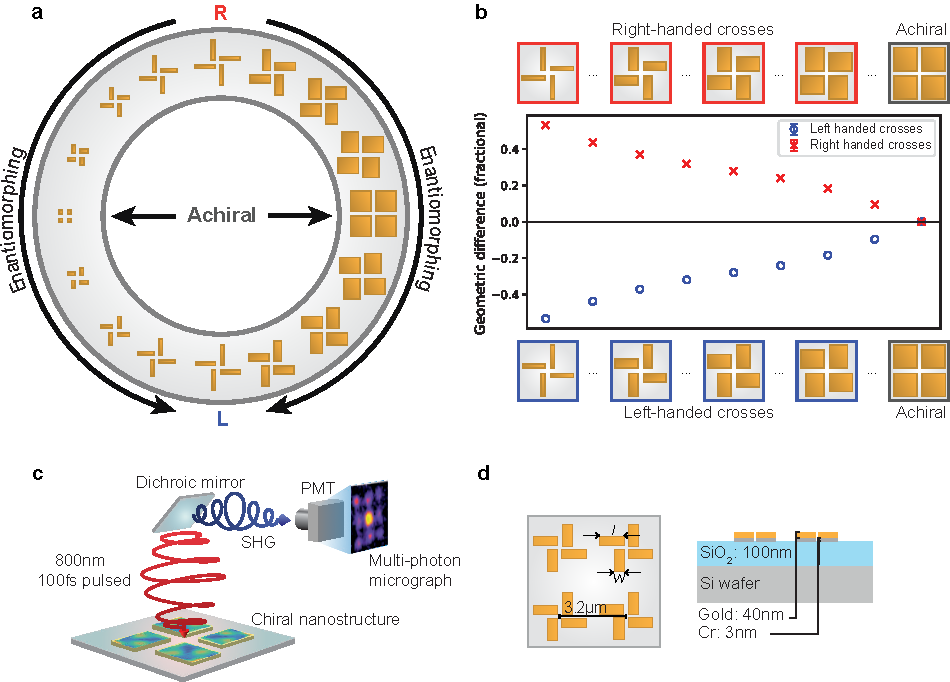
\includegraphics[scale=1]{./figures/results/EnantiomorphingChiralCrosses/setup.pdf}
    \caption{\label{fig:results:EnantiomorphingChiralCrosses:setup}
    \textbf{a)} Representation of two possible pathways to enantiomorph a right-handed structure (R) into a left-handed structure (L), through an achiral geometry. Here, we examine the pathway on the right side of the circle. \textbf{b)} As the left-handed chiral crosses change into achiral square structures and into right-handed chiral crosses, the chiral geometric difference diminishes until it reaches 0 in the achiral case and then reverse its value. \textbf{c)} Schematic diagram of the multiphoton microscopy experiments. \textbf{d)} Geometry and depth profile of the chiral crosses samples.}	
\end{figure}

Here, we developed an experiment impossible to perform with chiral molecules: by designing 35 intermediate geometries, we can ``enantiomorph'' plasmonic nanostructures from one handedness to the other, passing through an achiral geometry. 
We demonstrate a bisignate (of two signs) circular intensity difference (CID) due to enantiomorphing, rather than wavelength change, in the nonlinear emission from near-field hotspots. Contrary to what would be expected from pure geometric considerations, the nonlinear chiroptical signal is double-bisignate. A full modal analysis of the structures is combined with group theory in order to understand this result. 

We find that, regardless of their handedness, chiral nanostructures support plasmon modes that can be excited by both left and right circularly polarised (LCP and RCP) light. Furthermore, which modes are dominant (i.e., couple strongest to light) depends on the wavelength or the shape/dimensions of the nanostructure. Therefore, it is possible to engineer chiral nanomaterials that, at a given wavelength, can only be excited with the ``wrong'' direction of CPL. 
This allows the possibility of tuning a structures' chiroptical response by selecting particular electromagnetic modes, or sets of modes, among hundreds supported, which can enable more sensitive chiroptical control than what is currently available.

\section{Results}\label{sec:results:EnantiomorphingChiralCrosses:results}

Initially, it is useful to consider the geometric chirality of the nanostructure. From here on, we will refer to the crosses as either left- or right-handed, following the convention shown in figure~\ref{fig:results:EnantiomorphingChiralCrosses:setup}b. Starting with left-handed crosses, their geometry is morphed in discrete steps, first into achiral squares and then into right-handed chiral crosses (figure~\ref{fig:results:EnantiomorphingChiralCrosses:setup}b). 
For the purposes of comparison, a measure of ``chiral geometric difference'' describes the area of maximal overlap that can be achieved between left- and right-handed structures, by rotating and translating the two mirror-image shapes, relative to each other (Appendix~\ref{sec:appendix:ChiralGeoDiff}). 
As figure~\ref{fig:results:EnantiomorphingChiralCrosses:setup}b shows, the chiral geometric difference diminishes until it reaches 0, in the achiral case. This trend is intuitively expected for an enantiomorphing transition, and even matches previously reported optical experiments~\cite{Katzenelson2000}. However, generally the chiroptical properties of nanostructures depend on more than geometry alone. Without considering material effects, and the properties of the incident light, no direct connection can be assumed between chiral geometric difference and chiroptical effects. This measure of chirality contrasts the double-bisignate response found in the following nonlinear CID measurements.

For these experiments, we made use of a commercial multiphoton microscope with circularly polarised illumination at 800 nm, depicted schematically in figure~\ref{fig:results:EnantiomorphingChiralCrosses:setup}c. Note that ``dichroic'' in the context of a dichroic mirror means different reflectivities at different wavelengths, here used to prevent reflected light at $\SI{800}{\nano\m}$ from being collected. The collected light consisted mostly of the second-harmonic generation (SHG). Specifically, a bandpass filter allowing $\SI{390}{\nano\m}$ to $\SI{465}{\nano\m}$ light was used and, although this filter passes a small part of two-photon luminescence signal, the SHG signal is clearly dominant in this spectral range. Since these nonlinear optical processes are enhanced in the regions of strong local field (chapter~\ref{sec:background:NonlinearOptics}), they act as a sensitive far-field probe for local-field effects. 

The samples are chiral crosses made of Au, deposited by electron beam lithography (EBL) on a Si substrate with a thermal oxide layer, and whose dimensions and depth profile are given in figure~\ref{fig:results:EnantiomorphingChiralCrosses:setup}d. Each cross is composed of four separate nanostripes, with varying width $w$ and length $l$. The separation distance between nanostripes, at the centre of the crosses, is constant at $\SI{200}{\nano\m}$. The crosses are arranged in a $\SI{40}{\micro\m} \times \SI{40}{\micro\m}$ square array, with the distance between cross centres also kept constant at $\SI{3.2}{\micro\m}$. 

\begin{figure}[htb!]	
    \centering	
    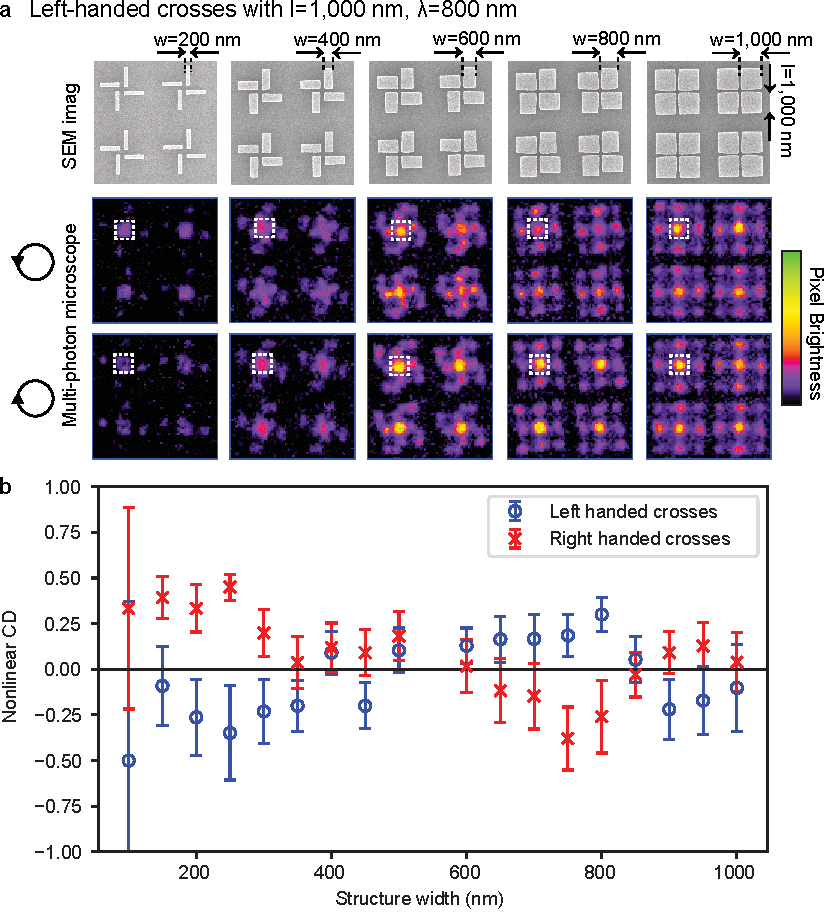
\includegraphics[scale=1]{./figures/results/EnantiomorphingChiralCrosses/l1000data.pdf}
    \caption{\label{fig:results:EnantiomorphingChiralCrosses:l1000data}
    Varying arm width of the nanostructure features at fixed l=1000nm. SEM images of 4 structure cells for each geometry \textbf{(a top)}, and SHG microscopy images \textbf{(a, lower)} under illumination from left (counter-clockwise arrow) and right (clockwise arrow) circularly polarised light, at $\SI{800}{\nano\m}$ wavelength. Scale (right) corresponds to image pixel brightness. \textbf{b)} Measured total nonlinear CID under $\SI{800}{\nano\m}$ wavelength light is then calculated for each geometry. Our experiments reveal a counter-intuitive behaviour for the second-harmonic generation circular intensity difference (SHG-CID) – both the 0 value and the reversal occur before reaching the achiral geometry.}	
\end{figure}

Figure~\ref{fig:results:EnantiomorphingChiralCrosses:l1000data}a shows scanning electron microscopy (SEM) images of sample arrays. In these arrays, the length of the nanostripes is fixed ($\SI{1000}{\nano\m}$) and the width changes from $\SI{200}{\nano\m}$ to $\SI{1000}{\nano\m}$ in steps of $\SI{200}{\nano\m}$. Below each SEM are two corresponding multi-photon micrographs, obtained with LCP and RCP. The multi-photon microscopy images are colour coded for intensity, and show bright hotspots at the centre of the chiral crosses (indicated with dashed-line squares for clarity). 
Similar hotspots have previously been observed at the centre of G-shaped \cite{Valev2009a} and S-shaped \cite{Valev2014} nanostructured arrays. 
The hotspots correspond to a chiral coupling at the centre of the unit cells that depends on the chirality of the nanostructures and the direction of CPL \cite{Valev2014, Petralli-Mallow1993, Byers1994}. This dependence is expressed as a directly observable nonlinear circular intensity difference. Interestingly though, in this set of samples, the nonlinear CID changes sign between the chiral crosses with nanostripe width  $\SI{200}{\nano\m}$ and $\SI{600}{\nano\m}$, even though the structures have the same handedness.

The nonlinear CID reversal can be seen more quantitatively in figure~\ref{fig:results:EnantiomorphingChiralCrosses:l1000data}b. Here, the nonlinear CID is obtained from the detected light upon LCP or RCP illumination according to 
$(I_{RCP}^{MP}-I_{LCP}^{MP})/(I_{RCP}^{MP}+I_{LCP}^{MP})$. The individual multi-photon intensity terms $I_{RCP}^{MP}$ and $I_{LCP}^{MP}$ were obtained from the pixel intensity at the centre of the chiral crosses, where the chiral coupling is maximum and the characteristic response is most pronounced. 
The nonlinear microscopy images obtained contain roughly 60 crosses of each type (left- and right-handed), with separate images for LCP and RCP illumination. A Python script was used to specify the central regions of 25 crosses, with clearly damaged structured avoided. For each cross, a 5-pixel by 5-pixel square at the defined central region was intensity-averaged (pixel array at $\SI{0.09}{\micro\m}$ per pixel). This result was itself then averaged over 25 crosses to obtain a final intensity and statistical uncertainty for a particular orientation of cross (left- or right-handed) and input polarisation (LCP or RCP). This was done for each of the considered geometries. 
It should be noted that the SEM pictures in figure~\ref{fig:results:EnantiomorphingChiralCrosses:l1000data}a are only a subset of the samples we studied. The full set started from $w= \SI{100}{\nano\m}$ and progressed to $w=\SI{1000}{\nano\m}$, in steps of $\SI{50}{\nano\m}$. 
Upon considering the nonlinear CID from all these samples, it is observed that between $w=\SI{200}{\nano\m}$ and $w=\SI{800}{\nano\m}$, the chiroptical response is unambiguously reversed, i.e. with clearly separated error bars. The nonlinear CID that we measured is collected in the far-field (well away from the structure surface), and it is very different from the \textit{linear} circular dichroism in the far-field. 

The linear far-field CID response is demonstrated by FDTD simulations data, shown in figure~\ref{fig:results:EnantiomorphingChiralCrosses:reflectionsim}. Additional linear scattering spectra simulations and experimental data are given in Appendix~\ref{sec:appendix:CrossesScatteringSpectra}. The data in figure~\ref{fig:results:EnantiomorphingChiralCrosses:reflectionsim} differ significantly from those in figure~\ref{fig:results:EnantiomorphingChiralCrosses:l1000data}b. A key reason for this difference is that the nonlinear CID originates in the near-field, strongly depending on the field intensity at the surface of the structure. To understand the observed reversal of the nonlinear CID, we need to examine the electromagnetic behaviour at the surface of the nanostructures. 

\begin{figure}[htb!]	
    \centering	
    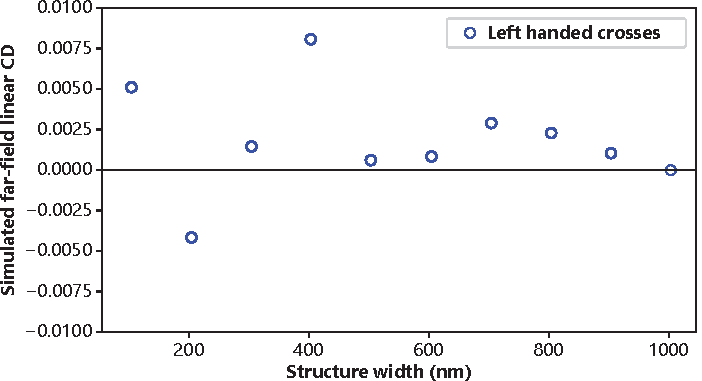
\includegraphics[scale=1]{./figures/results/EnantiomorphingChiralCrosses/reflection_sim.pdf}
    \caption{\label{fig:results:EnantiomorphingChiralCrosses:reflectionsim}
    Simulated far-field linear reflection CD for left-handed chiral cross structures. The lineshape of the linear CD response is significantly different to that obtained from nonlinear CID measurements.}	
\end{figure}

\section{Discussion}\label{sec:results:EnantiomorphingChiralCrosses:discussion}

\begin{figure}[htb!]	
    \centering	
    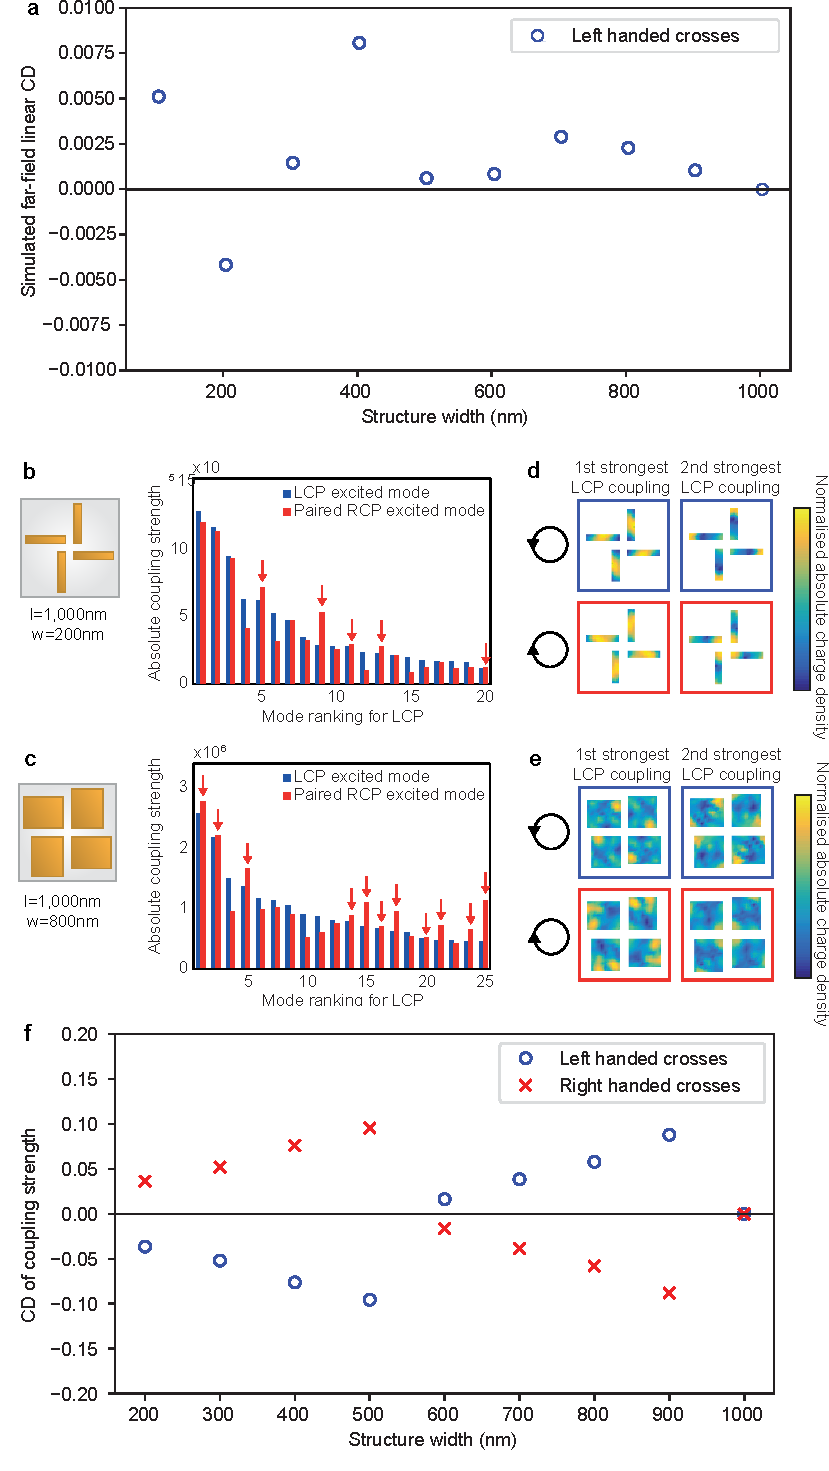
\includegraphics[scale=1]{./figures/results/EnantiomorphingChiralCrosses/l1000modes.pdf}
    \caption{\label{fig:results:EnantiomorphingChiralCrosses:l1000modes}
    \textbf{a-e}. Simulation results showing modal composition of chiroptical response. Modal analysis of structures with arm length 1000nm, width 200nm \textbf{(a)} and 800nm \textbf{(b)}. The most LCP-dominant modes for each structure are plotted showing both LCP coupling strength (blue) and the correlated-mode RCP coupling strength (red). Modes coupling stronger to RCP than LCP are marked with arrows. Examples of individual modes (normalized absolute charge density) are shown for width $\SI{200}{\nano\m}$ \textbf{(c)} and 800nm \textbf{(d)}. The total coupling strength CID as defined in equation~\ref{eq:background:ChiropticalEffects:couplingCD} is plotted for varying arm width, at fixed $l=\SI{1000}{\nano\m}$ under $\SI{800}{\nano\m}$ wavelength light \textbf{(e)}.}	
\end{figure}

For each nanostructure examined, the induced current flowing in the structure due to an incident field was obtained by X. Zheng and G. A. E. Vandenbosch using the methods detailed in references \cite{Collins2018, Zheng2012}. For a given structure, the full induced current solution $\mathbf{J}$ is characterised by a set of modes $\mathbf{J_n}$ and corresponding eigenvalues $\lambda_{n}$. Each structure is associated with a different set of modes, and the amplitudes of each mode describe their coupling strengths to a particular incident field.
These methods are well established, but here the analysis was taken further by making use of group theory. Each available mode associated with a given structure geometry can be placed in one of four orthogonal irreducible representations $\Gamma _{j = 1,2,3,4}$. These representations correspond to exclusive excitation with either the two orthogonal linear polarisations ($\Gamma _{1}$ for horizontal and $\Gamma _{2}$ for vertical) or the two circular polarisations ($\Gamma _{3}$ for LCP and $\Gamma _{4}$ for RCP). 
Importantly, each mode in the 3rd irreducible representation has a ``correlated'' mode in the 4th irreducible representation, with identical eigenvalues forming an ``accidentally degenerate pair''. 
Crucially, the LCP coupling coefficient of a given $\Gamma _{3}$ mode may be different from the RCP coupling coefficient of the correlated $\Gamma _{4}$ mode. 
This difference in a mode pair's ability to couple to LCP and RCP incident light can be seen as a type of modal CID, and is shown in figure~\ref{fig:results:EnantiomorphingChiralCrosses:l1000modes}a, b. 

Figure~\ref{fig:results:EnantiomorphingChiralCrosses:l1000modes}a shows pairs of correlated modes in the structures with width $\SI{200}{\nano\m}$. In blue, the $\Gamma _{3}$ modes are ranked according to their coupling coefficient to LCP. The correlated $\Gamma _{4}$ modes, which only couple to RCP, are shown in red. In an achiral structure, both the blue and red sets would have identical values and ranking. Not surprisingly, the presence of chirality in the structure breaks the symmetry and, overall, the blue modes have higher coupling coefficients. 
But counter-intuitively, we also find that, in some pairs, the red modes have higher coupling coefficients. This means that, for such modes, light of the ``wrong chirality'' couples more efficiently to the chirality of the nanostructure. An example of this behaviour is indicated with an arrow on the figure. As we will see next, the exception can become the rule as we continue changing the cross width towards an achiral structure.

Figure~\ref{fig:results:EnantiomorphingChiralCrosses:l1000modes}b shows pairs of correlated modes in the structures with width $\SI{800}{\nano\m}$. Here, there are more red-dominant pairs of correlated modes than in figure~\ref{fig:results:EnantiomorphingChiralCrosses:l1000modes}a, to the point that the overall calculated near-field CID is reversed, as in the experimental observation. Therefore, in these plasmonic nanostructures, the chiroptical response originates from the superposition of all the individual modal responses. 
The modes themselves represent complex spatial distributions of the charge density; as an illustration, the first and second modes from figure~\ref{fig:results:EnantiomorphingChiralCrosses:l1000modes}a and \ref{fig:results:EnantiomorphingChiralCrosses:l1000modes}b are shown in figure~\ref{fig:results:EnantiomorphingChiralCrosses:l1000modes}c and \ref{fig:results:EnantiomorphingChiralCrosses:l1000modes}d, respectively.
Since the near-field intensity is directly related to the total charge density, regions of high charge density will result in SHG hotspots (via local fields) on the structure surface. Therefore, differences in the coupling of charge density modes to LCP and RCP light are directly responsible for the observed SHG-CID.

Mathematically, the overall near-field CID originates from the full solution $\mathbf{J}$ obtained by linearly superposing the contributions from all eigenmodes $\mathbf{J_n}$~\cite{Zheng2014}, 

\begin{equation}\label{eq:background:ChiropticalEffects:totalSolution}	
	\mathbf{J} (\mathbf{r}, \omega) = \sum \limits_{n} c_{n}(\omega) \mathbf{J_{n}}(\mathbf{r}, \omega).
\end{equation}

Here, $\mathbf{J}$ represents the current flowing at an observation point $\mathbf{r}$ in the nanostructure induced by an incident field $\mathbf{E}(\mathbf{r}, \omega)$ oscillating at a frequency $\omega$. For a given incident field, the coupling coefficients $c_n$ are given by~\cite{Zheng2015, Zheng2014}
\begin{equation}\label{eq:background:ChiropticalEffects:couplingCoefficients}	
	c_n(\omega) = \frac{\int_{V} \mathbf{J}(\mathbf{r}, \omega) \cdot \mathbf{E}(\mathbf{r}, \omega) d\mathbf{r}}{\lambda_{n}(\omega)}
\end{equation}
and the volume integration $\int_{V}$ is carried out over the whole nanostructure~\cite{Zheng2013}. 
To calculate an overall near-field CID, we make use of the inner product of the coupling coefficients given by
\begin{equation}\label{eq:background:ChiropticalEffects:couplingInnerProduct}	
	\left\| c_{n}(\omega ) \right\| = \left\langle c_{n}(\omega),c_{n}(\omega) \right\rangle = \sum\limits_n c_{n}(\omega) c_{n}^* (\omega)
\end{equation}
Here, $c_{n}^*$ denotes the complex conjugate of $c_{n}$.
Since the local-field intensity is dependent on the square of all coupling coefficients, the local-field circular-dichroism can be expressed as
\begin{equation}\label{eq:background:ChiropticalEffects:couplingCD}	
	\mathrm{CID}^{(Local)} \propto \frac{{\left\| {{c_n}^R(\omega )} \right\|}^2 - {\left\| {{c_n}^L(\omega )} \right\|}^2}{{\left\| {{c_n}^R(\omega )} \right\|}^2 + {\left\| {{c_n}^L(\omega )} \right\|}^2}.
\end{equation}
The \textit{L} and \textit{R} superscripts refer to the solutions for LCP and RCP respectively. 
The results from equation~\ref{eq:background:ChiropticalEffects:couplingCD} can be found in figure~\ref{fig:results:EnantiomorphingChiralCrosses:l1000modes}f, where the calculated near-field CID is plotted as a function of the nanostripe width ($w$), for the left-handed and right-handed crosses. These numerical results show a bisignate near-field CID response corresponding well to the experimental nonlinear CID curves in figure~\ref{fig:results:EnantiomorphingChiralCrosses:l1000data}b. 
While figure~\ref{fig:results:EnantiomorphingChiralCrosses:l1000data}a reveals slight deformation towards the centre of the measured crosses, for large ($>\SI{400}{\nano\m}$) cross widths, the effect of this deformation on the SHG-CID is minor (see reference~\cite{Valev2014}). 
The bisignate trend seen in Figure~\ref{fig:results:EnantiomorphingChiralCrosses:l1000modes}f is in good agreement with the experimental data found in figure~\ref{fig:results:EnantiomorphingChiralCrosses:l1000data}b.

\begin{figure}[htb!]	
    \centering	
    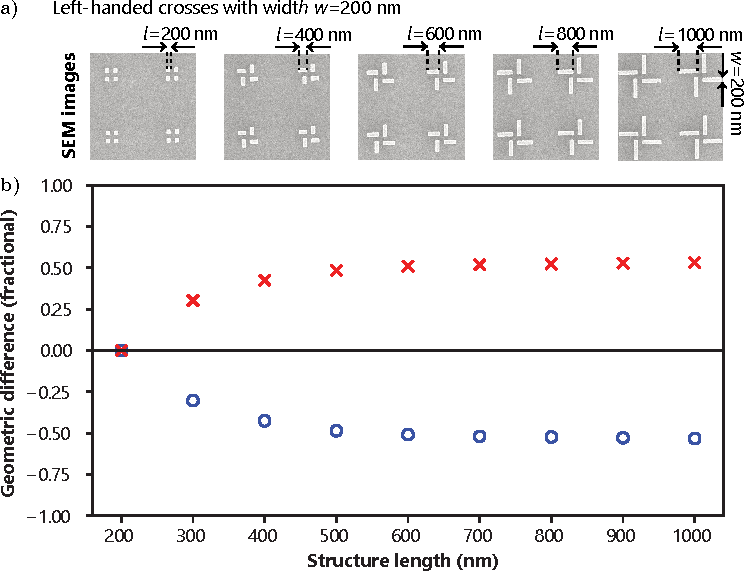
\includegraphics[scale=1]{./figures/results/EnantiomorphingChiralCrosses/d200structures.pdf}
    \caption{\label{fig:results:EnantiomorphingChiralCrosses:d200structures}
    Additional experimental and simulated CID results. Varying arm length of the nanostructure features at fixed $w=\SI{200}{\nano\m}$. \textbf{a)}. SEM images of 4 structure cells for each geometry. \textbf{b)}. Chiral geometric difference for structures of fixed arm width $w=\SI{200}{\nano\m}$.}	
\end{figure}

This agreement was further verified with a second set of intermediate structures (figure~\ref{fig:results:EnantiomorphingChiralCrosses:d200structures}) in which the nanostripe length is varied, for a constant width of $\SI{200}{\nano\m}$. We observe in both the experiments (originating from near-field) and the near-field simulations that the CID emerges away from the achiral structure, and subsequently plateaus (figure~\ref{fig:results:EnantiomorphingChiralCrosses:d200data}). Although longer nanostripes support more electromagnetic modes than shorter ones, these additional modes spread across the whole structure, and do not influence dramatically the key central region. The nonlinear CID measurements probe the the centre of the crosses and, consequently, it plateaus as nanostripe length increases.

\begin{figure}[htb!]	
    \centering	
    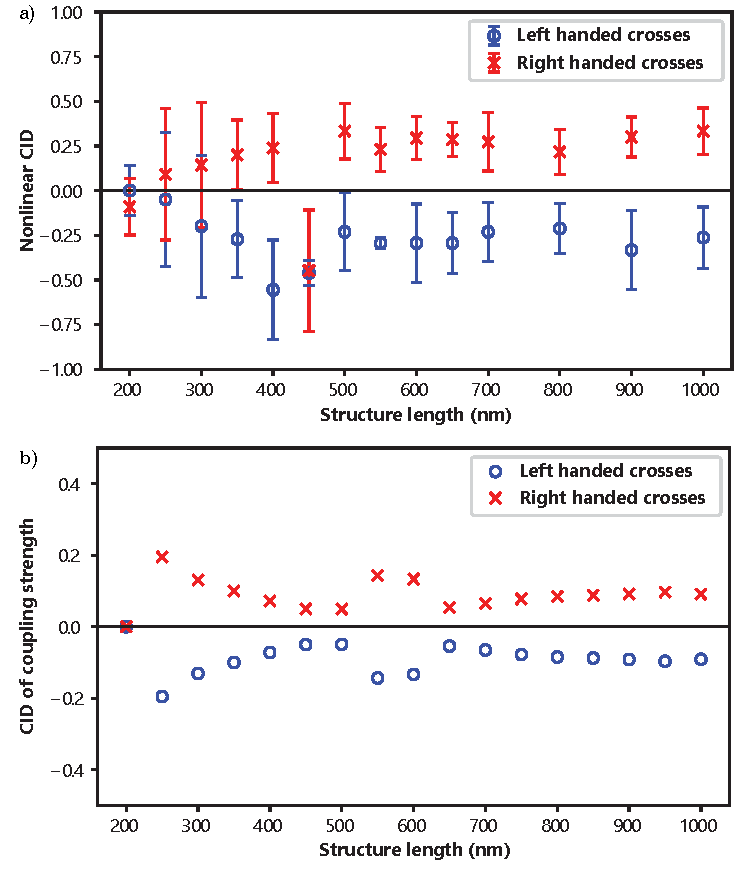
\includegraphics[scale=1]{./figures/results/EnantiomorphingChiralCrosses/d200data.pdf}
    \caption{\label{fig:results:EnantiomorphingChiralCrosses:d200data}
    Additional experimental and simulated CID results. Varying arm length of the nanostructure features at fixed $w=\SI{200}{\nano\m}$. \textbf{a)} Measured total multi-photon CID, and \textbf{(b)} total coupling strength CID obtained from modal analysis, under $\lambda=\SI{800}{\nano\m}$ wavelength light is then calculated for each geometry. Unlike the case of fixed length and varying width, no bisignate CID is observed here, more closely matching the chiral geometric difference.}
\end{figure}

\section{Conclusions}\label{sec:results:EnantiomorphingChiralCrosses:conclusions}

This chapter has focussed on the bisignate CID response as a function of varying a structure's geometry. With respect to wavelength, both linear and nonlinear chiroptical spectra often exhibit complex bisignate features~\cite{Li2015, Lee2013, Decker2007, Droulias2013, Plum2009}. This behaviour can be linked to Kuhn's sum-rule~\cite{Kuhn1930}, which states that the chiroptical response must be zero over all wavelengths. This dependence on wavelength has been analysed in terms of exciton coupling~\cite{Guerrero-Martinez2011} nanoparticle-nanoparticle Coulomb coupling~\cite{Fan2010}, and energy level hybridisation~\cite{Auguie2011a}.
In particular, in the linear optical case it was shown that the energetic ordering of the hybridised modes can be changed, resulting in a reversal of the linear CD, upon making small relative position shifts between L-shaped nanoparticles~\cite{Hentschel2015}.
In the context of our group-theory discussion, the coupling coefficients of each mode pair are highly dependent on the wavelength of light. Changing the wavelength will change which mode pairs are dominant within the set, for a particular structure geometry. In principle, this can also be used to optimise the CID for a fixed structure and variable wavelength. However, it is often desirable, or even necessary, to operate at a particular wavelength, for example if probing molecules attached to the nanostructure surface. In these cases, tuning the structure geometry allows the near-field CID to be optimised around the available wavelength.

In this work, it has been shown that the origin of the chiroptical response in plasmonic nanostructures can be described by the selective excitation of available surface plasmon modes. Therefore, any physical property that affects the modes will allow tuning of the chiroptical response. This mechanism could also be used to explain previous experimental observations of bisignate CID spectra, where different sets of modes can be coupled differently depending on the wavelength of light. Furthermore, we predict that variation of temperature of the nanostructures (e.g. by laser heating) will change the sets of available modes, due to thermal expansion or a change in permittivity~\cite{Aksyutov1977}, and can lead to tuning the chiroptical response. Further physical processes that involve excitation of specific plasmonic modes (Fano resonance, spasers, electromagnetically induced transparency, etc.) can also be used to tune that response for desired applications. 
In practice, maximising the chiroptical response in any plasmonic nanostructure is allowed by suppression of the modes that couple to light ``with the wrong chirality''. Equally important, by locally enhancing a particularly strong mode (e.g. via coupling to an auxiliary structure) it may be possible to enhance the chiroptical interaction with molecules. In many cases, these molecular interactions will occur at specific wavelength ranges. In this chapter it is shown that the chiroptical response at a specific wavelength can be enhanced, and even reversed, by tuning structure geometry alone. This tuneability will lead to improved enantioselectivity for molecular sensing, separation and synthesis.

\chapter{Optical Activity in Plasmonic Metasurfaces}\label{sec:results:OAinPlanarNanohelices}

Sections of this chapter have been copied verbatim from the (published) manuscript \textit{``Second Harmonic Generation Optical Rotation Solely Attributable to Chirality in Plasmonic Metasurfaces''}, Joel~T.~Collins et. al. \cite{Collins2018b}.
V. K. Valev designed the nonlinear experimental setup. A.G.Mark fabricated the samples. SHG data were collected by myself, and D. C. Hooper. Linear optical data were collected by myself and C. Kuppe. I analysed both the SHG and linear data. Tensor analysis and analytical verification of experimental results were performed by myself. I produced the manuscript draft on which this chapter is based.

\bigskip \noindent
As discussed in section~\ref{sec:background:Chirality:anisotropy}, both linear and nonlinear optical rotation can occur even in achiral structures, if the structure is birefringent due to anisotropy, making pure chiral information difficult to obtain~\cite{Hooper2017}. Crucially however, chiroptical effects resulting from anisotropy exhibit a strong dependence on structural orientation. Here we report large second-harmonic generation optical rotation of $\pm\SI{45}{\degree}$, due to intrinsic chirality in a highly anisotropic helical metamaterial. The SHG intensity is found to depend strongly on the structural anisotropy, however the angle of SHG-OR is invariant under sample rotation. The results show that by tuning the geometry of anisotropic nanostructures, the interaction between anisotropy, chirality, and experiment geometry can allow greater control over the chiroptical properties of plasmonic metamaterials.

\section{Introduction}\label{sec:results:OAinPlanarNanohelices:introduction}
In this set of experiments, we made use of chiral optical metamaterials (section~\ref{sec:background:Plasmonics:Metamaterials}), whose properties are determined by both the choice of materials, and their geometry. Previously, large plasmon-enhanced linear CD and OR effects have been reported in chiral metamaterials \cite{Decker2007, Papakostas2003, Kuwata-Gonokami2005a, Plum2007, Gansel2011}.
Because CD and OR originate from the real and imaginary part of the refractive index, respectively, the two effects are linked by the Kramers-Kronig transforms (section~\ref{sec:background:Chirality:Chiroptics}).
However, this link is not necessary for nonlinear chiroptical effects; since nonlinear CID and OR do not result from the real and imaginary parts of a single complex number.

For second harmonic generation (SHG), the two nonlinear chiroptical effects SHG-CID and SHG-OR are fundamentally different from, and can be highly complementary to, linear chiroptical effects. For the latter, interacting parallel components of electric and magnetic dipoles are strictly necessary. This necessity is lifted in the nonlinear case. Since SHG is a three-wave mixing process, chiroptical effects can arise from the 3D chiral arrangement of electric dipoles only~\cite{verbiest2009second}. 
SHG chiroptical effects can also originate from the interaction between electric and magnetic dipoles, as well as between electric dipoles and quadrupoles. This specificity allows SHG to discriminate between two principal models of chirality~\cite{Fischer2005a}: Kuhn's ``chirally-coupled dipoles''~\cite{Kuhn1930} and Kauzmann's ``one electron on a helix''~\cite{Kauzmann1957a} models. More precisely, the two can be separated by measuring SHG-OR. 

Whereas SHG-CID has been demonstrated from numerous chiral nanomaterials \cite{Hooper2017, Mamonov2017, Chen2016, Kolkowski2015, Belardini2014}, far less attention has been devoted to SHG-OR. Previous studies have demonstrated SHG-OR in plasmonic nanostructures, where the origin of the effect can be ambiguous~\cite{Romain2017, Ren2012a, Mamonov2012}, since SHG-OR can originate from both intrinsic chirality and anisotropy. An unambiguously chiral origin of SHG-OR has not been previously reported in nano/meta-materials. 

\section{Results}\label{sec:results:OAinPlanarNanohelices:results}
Here, we demonstrate clear SHG-OR in plasmonic metamaterials, which is due to intrinsic chirality; the SHG-OR angle does not depend on the sample rotation angle and it reverses upon mirroring the geometry. Conversely, for the same sample, the linear OR angle depends strongly on the rotation of the sample, which demonstrates a dominant contribution from anisotropy rather than chirality, in the linear case. Moreover, we show that SHG-OR can also be dominantly sensitive to the anisotropy of the samples, depending on the experimental geometry and on the particular values of the nonlinear susceptibility tensor components involved. 

The samples used in these experiments are arrays of hexagonally-arranged Au:Cu (80:20) nanohelices, fabricated by A.G.Mark using a glancing-angle shadow growth method \cite{Gibbs2014}. The structures are shown schematically and in a cross-sectional SEM image in figure~\ref{fig:results:OAinPlanarNanohelices:setup}a and figure~\ref{fig:results:OAinPlanarNanohelices:setup}(b) respectively. 
Only one handedness of the structures is shown, however both left- and right-handed nanohelices were investigated. The individual nanohelices have a pitch of $\SI{37}{\nano\m}$, and height of $\SI{81}{\nano\m}$, a wire thickness of $\SI{18}{\nano\m}$, and the nanohelices have an inner and outer diameter of $\SI{28}{\nano\m}$ and $\SI{55}{\nano\m}$, respectively. Consequently, the structures are substantially sub-wavelength ($\approx\lambda/10$, at 800 nm).
The experimental setup (shown schematically in figure~\ref{fig:results:OAinPlanarNanohelices:setup}c) was designed to precisely measure the polarization of SHG emission from the samples. 

$\SI{8.4}{\milli\watt}\pm\SI{0.1}{\milli\watt}$ of pulsed light centered at $\SI{800}{\nano\m}$ ($\SI{62}{\kilo\watt}$ peak power, appendix~\ref{sec:appendix:hardware:maitai}) was directed to a half-wave plate and rotated to a specific linear polarization angle. An RG665 long pass filter removed any existing SHG from the beam, before an achromatic lens focused the $\SI{800}{\nano\m}$ light onto our sample at $\SI{45}{\deg}$ incidence. A BG39 filter then removed reflected $\SI{800}{\nano\m}$ light, passing only the $\SI{400}{\nano\m}$ SHG emission which was then collimated by another lens. The SHG emission then passed through an analyzing polarizer, before being focused onto a photomultiplier tube (PMT). The PMT output is pre-amplified and sent to an SRS SR400 Gated Photon Counter. 
By varying both the sample azimuthal rotation angle and the analyzing polarizer angle, a heatmap is produced. The latter shows the intensity of SHG emission, as a function of both sample rotation (along the $y$-axis) and analyzer rotation (along the $x$-axis). 

\begin{figure}[htb!]	
    \centering	
    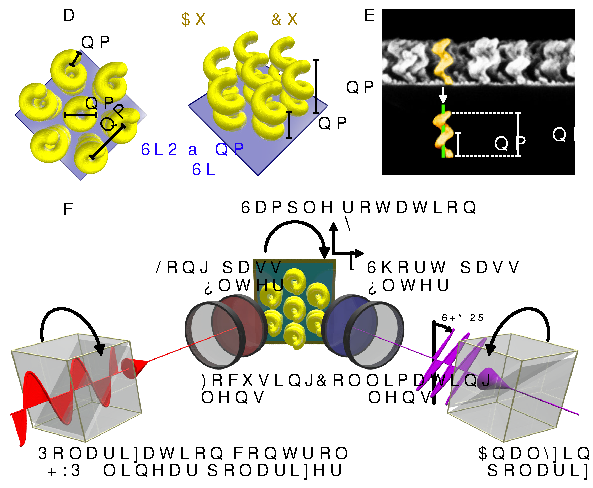
\includegraphics[scale=1.0]{./figures/results/OAinPlanarNanohelices/setup.pdf}
    \caption{\label{fig:results:OAinPlanarNanohelices:setup}
    \textbf{a)} Schematic diagram of one handedness of nanohelix array, showing structure spacing $\SI{55}{\nano\m}$, height $\SI{81}{\nano\m}$, and pitch $\SI{37}{\nano\m}$. \textbf{b)} Side-on SEM of the metamaterial surface, of the same handedness. A single helix has been highlighted for clarity. \textbf{c)} Schematic of experimental setup, showing S-polarized $\SI{800}{\nano\m}$ incident light. For optical rotation measurements, the analyzing polarizer is continuously rotated, for a series of sample azimuthal rotations.}	
\end{figure}

Figure~\ref{fig:results:OAinPlanarNanohelices:s_data} shows SHG hotspots corresponding to the polarization of SHG emission as the sample is rotated. The green markers on Figure~\ref{fig:results:OAinPlanarNanohelices:s_data} show the angle of SHG polarization for each sample rotation angle. Relative to the incoming S-polarized (perpendicular to the plane of incidence) light, an SHG-OR of approximately $+\SI{45}{\degree}$ is observed for the left-handed structures. Importantly, the SHG-OR angle does not change significantly over regions of strong SHG emission.
Moreover, upon measuring the right-handed structures, the SHG-OR reverses to approximately $-\SI{45}{\degree}$. While the data for the right-handed structure are noisier due to slight sample damage, the results are still clear. The reversal is exactly as expected for SHG-OR due to intrinsic chirality. The intensity of SHG emission does vary sinesoidally with rotation, suggesting a dipole coupling between the incident light and the end terminations of the nanohelices. After coupling into the structures via the end termination, the polarisation of light is then rotated by the intrinsic chirality of the helical structure.


\begin{figure}[htb!]	
    \centering	
    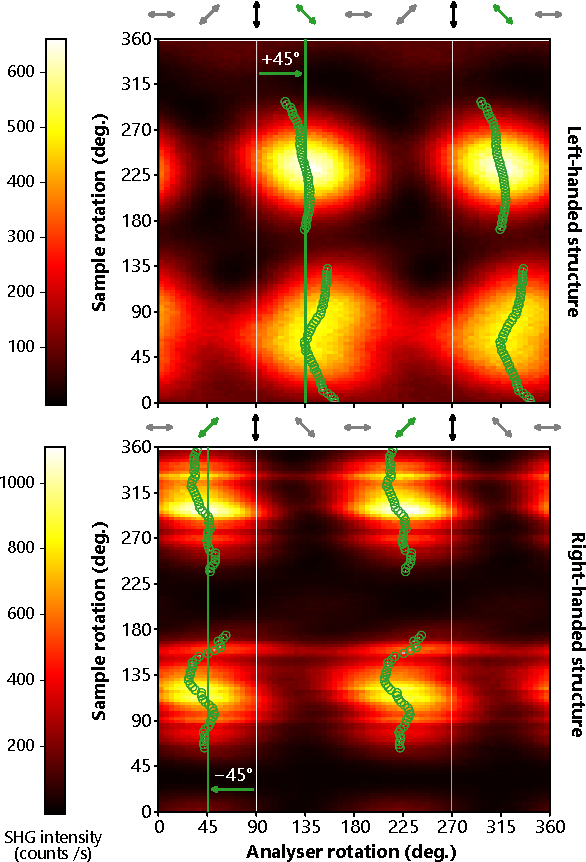
\includegraphics[scale=1]{./figures/results/OAinPlanarNanohelices/s_data.pdf}

    \caption{\label{fig:results:OAinPlanarNanohelices:s_data}
    SHG optical rotation heatmaps for both enantiomorphs of helical metamaterial. S-polarized incident light results in rotated linearly polarized SHG emission. By continuously rotating the analyzer, the angle of maximum intensity at each sample rotation can be obtained (shown in green markers). For the left-handed structure an SHG-OR angle of around $+\SI{45}{\degree}$ is found. In the mirrored, right-handed structure, the SHG-OR changes sign, to around $-\SI{45}{\degree}$. Importantly, in both cases the angle remains relatively unchanged upon sample rotation, though the overall intensity varies periodically.}	
\end{figure}

\begin{figure}[htb!]	
    \centering	
    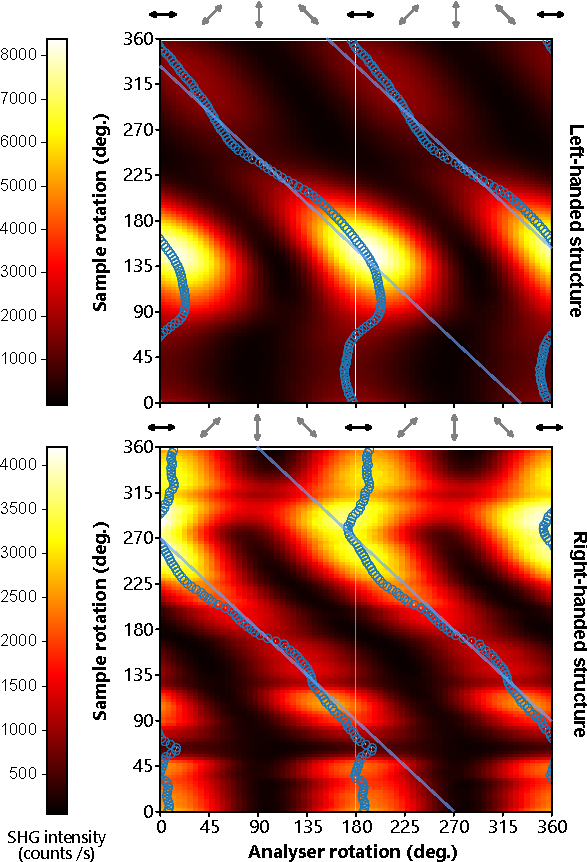
\includegraphics[scale=1]{./figures/results/OAinPlanarNanohelices/p_data.pdf}

    \caption{\label{fig:results:OAinPlanarNanohelices:p_data}
    SHG optical rotation heatmap for both enantiomorphs of the helical metamaterial, for P-polarized (parallel to the plane of incidence) incident light. In this case, both the angle of SHG-OR and the intensity of SHG emission are strongly dependent on sample rotation. Additionally, there is no clear reversal between enantiomorphs of the metamaterial. Instead, the sign of SHG-OR reverses under sample rotation, suggesting contributions from anisotropy dominating over contributions from the structure's intrinsic chirality.}	
\end{figure}

Importantly however, SHG-OR is not always independent of sample anisotropy. As discussed in section~\ref{sec:results:OAinPlanarNanohelices:discussion}, SHG is a highly symmetry-sensitive technique, whereby symmetry is expressed in the values of nonlinear susceptibility tensor elements. Depending on the experimental geometry, and on the values of these tensor elements, competing symmetries within the structure can be dominant in the measured results. This is directly demonstrated in figure~\ref{fig:results:OAinPlanarNanohelices:p_data}. 
The data presented in figure~\ref{fig:results:OAinPlanarNanohelices:p_data} were obtained from the same nanohelices, however whereas in figure~\ref{fig:results:OAinPlanarNanohelices:s_data} we used S-polarized light, here P-polarized light was employed. As in figure~\ref{fig:results:OAinPlanarNanohelices:s_data}, the heat maps correspond to SHG intensity as a function of sample and analyzer rotation angles. Contrary to figure~\ref{fig:results:OAinPlanarNanohelices:s_data}, the SHG-OR angle changes significantly over the regions of SHG emission, closely following the sample rotation angle. This behavior is exactly as expected for SHG-OR dominantly due to sample anisotropy. The experimental geometry must be carefully selected to address the structural chirality exclusively. 
Furthermore, additional data presented in Appendix~\ref{sec:appendix:AdditionalAuHelix} demonstrate that the precise experimental conditions required to isolate instrinsic chirality, and anisotropy, depend strongly on the geometry of the nanomaterial. We observe that changes in the nanohelix separation have a large impact on the nonlinear optical activity, entangling the effects of chirality and anisotropy. Changes in the nanohelix dimensions with the same separation have a less dramatic effect, preserving the anisotropy-dominated SHG-OR under p-polarised illumination, but also exhibiting no behaviour \textit{exclusively} attributable to chirality.

The nonlinear chiroptical behavior reported here is in stark contrast to the linear chiroptical case. The linear OR of the nanohelices was investigated with optical microscopy and spectroscopy. 
Microscopy images were obtained on a commercial Zeiss Axio Imager M2m wide-field microscope, with a halogen lamp for illumination. Images were taken in bright-field reflection mode, through an Epiplan-Neofluar $20\times$/0.50 HD DIC objective, using an Axiocam 105 color camera. Incident polarisation was controlled using a fixed Zeiss linear polariser slider, with the output image analysed with a Zeiss $\SI{360}{\deg}$ rotatable analyser slider. 
The analyser can be precisely rotated through $\SI{360}{\degree}$. Under crossed polariser geometry, only light that has experienced OR reaches the detector. By rotating the analyser, the sign of this OR can be obtained. 


Figure~\ref{fig:results:OAinPlanarNanohelices:lin_data}a shows a $3 \times 3$ array of optical microscopy images (in color) of the nanohelices. The rows correspond to three different sample rotation angles ($\SI{0}{\degree}$, $\SI{45}{\degree}$ and $\SI{90}{\degree}$) and the columns corresponds to three analyser rotation angles ($\SI{85}{\degree}$, $\SI{90}{\degree}$, $\SI{95}{\degree}$).
The sign of OR is revealed by color contrast in the images. For a sample oriented at $\SI{0}{\degree}$ and an analyser positioned at $\SI{85}{\degree}$, the image appears green.
Upon rotating the analyser to $\SI{95}{\degree}$, the color changes to red. However, upon orienting the sample at $\SI{90}{\degree}$, the color contrast reverses, indicating an opposite OR. This behavior suggests that the angle of OR depends on sample orientation and that OR changes sign every $\SI{90}{\degree}$. 
This trend is confirmed in figure~\ref{fig:results:OAinPlanarNanohelices:lin_data}b, showing an OR spectral map, obtained by rotating the sample between crossed polarizers. 
Spectra were obtained by diverting the microscope image to a collection lens focusing onto a $\SI{400}{\micro\m}$ diameter multimode optical fiber. The output of the fiber was connected to an Ocean Optics QE Pro commercial spectrometer, running with a $\SI{500}{\milli\s}$ integration time. The spectral data is normalized to account for the spectral lineshape of our halogen lamp source. Reference spectra were obtained using a silver mirror to measure the spectral lineshape of the source only. The measured metamaterial spectra were divided by this reference to give spectra independent of the illumination source.
Here, a $\SI{90}{\degree}$ rotational periodicity for the OR is clearly visible, at wavelengths above $\SI{550}{\nano\m}$. The behavior of the sample is consistent with that of a radiating dipole rotated through $\SI{360}{\degree}$. Such a dipole can be situated at the end-termination of the nanohelices. In the ranges of study, this dipole is excited by wavelengths from $\SI{550}{\nano\m}$ to $\SI{800}{\nano\m}$. The latter is the fundamental wavelength used for the SHG data in Figures~\ref{fig:results:OAinPlanarNanohelices:s_data} and~\ref{fig:results:OAinPlanarNanohelices:p_data}, where the SHG intensity also depends on coupling to the end-termination dipole, as discussed above.

\begin{figure}[htb!]	
    \centering	
    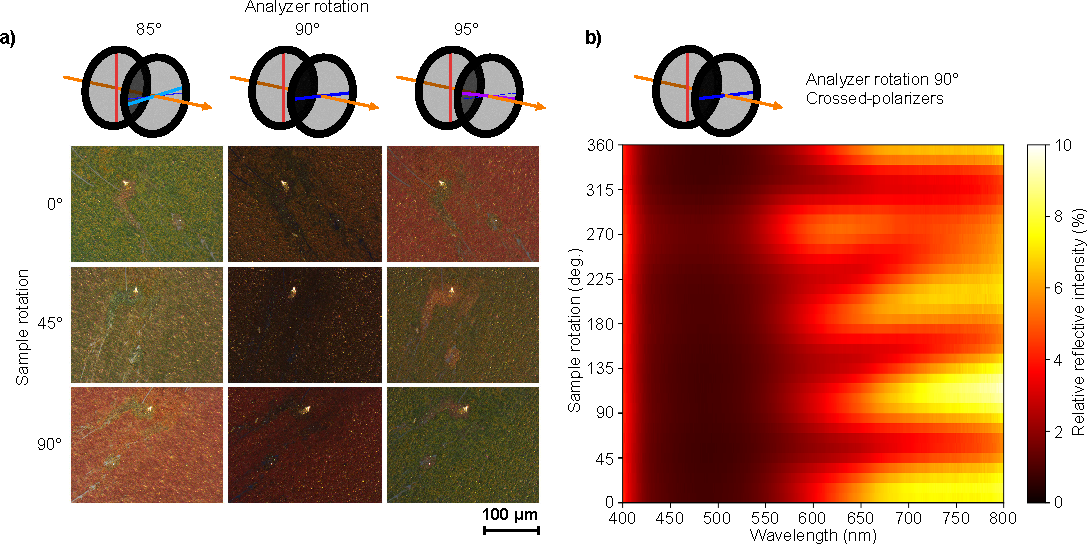
\includegraphics[scale=1]{./figures/results/OAinPlanarNanohelices/lin_data.pdf}

    \caption{\label{fig:results:OAinPlanarNanohelices:lin_data}
    Linear optical rotation data obtained through microscopy. \textbf{a)} Microscopy images of left-handed structure under illumination by linearly polarized white light, with various almost-crossed analyzing polarizer angles. By rotating the analyzer slightly away from crossed ($\SI{90}{\degree}$), the spectral dependence of optical rotation can be observed. Longer wavelengths are transmitted more through the analyzer when oriented at $+\SI{5}{\degree}$ away from crossed. Upon rotating the structure by $\SI{90}{\degree}$ the OR reverses. \textbf{b)} Linear OR map obtained from a spectrometer connected to the microscope viewport, showing clear dependence on sample rotation. Since the sample is between crossed polarizers, positive and negative OR both increase the measured intensity.}
\end{figure}

\section{Discussion}\label{sec:results:OAinPlanarNanohelices:discussion}
Due to the sub-wavelength dimensions and separation of nanostructure inclusions, our sample can be treated as an effective dielectric medium, described by effective susceptibility tensors as in section~\ref{sec:background:NonlinearOptics:susceptibility}.
At a given optical frequency $\omega$, the nonlinear chiroptical effects are described in terms of the nonlinear susceptibility tensors, relating the induced polarization ($P$) at the second-harmonic ($2\omega$) to the driving electric ($E$) and magnetic ($B$) fields, by equation~\ref{eq:results:OAinPlanarNanohelices:P2contributions}.
\begin{equation}\label{eq:results:OAinPlanarNanohelices:P2contributions}	
    {P_i}\left( {2\omega } \right) = 
    \varepsilon{_0}\chi_{ijk}^{eee}{E_j}\left(\omega \right){E_k}\left(\omega \right) + \varepsilon{_0}\chi_{ijk}^{eem}{E_j}\left(\omega \right){B_k}\left(\omega \right) + \varepsilon{_0}\chi_{ijk}^{eme}{B_j}\left(\omega \right){E_k}\left(\omega \right)
\end{equation}
The indices $i$, $j$, and $k$ describe the Cartesian directions of the fields, and can represent $x$, $y$, or $z$ (see figure~\ref{fig:results:OAinPlanarNanohelices:setup}c). 
The superscripts $e$ and $m$ stand for electric and magnetic dipole transitions, respectively, while $\varepsilon{_0}$ is the permittivity of vacuum. 
In addition to equation~\ref{eq:results:OAinPlanarNanohelices:P2contributions}, the incident electromagnetic fields can induce a magnetization $M_i$ analogous to the polarization $P_i$. 
In our experiment (figure~\ref{fig:results:OAinPlanarNanohelices:s_data}), the incident electric field is polarized perpendicularly to the main helix axis, therefore this magnetic contribution is excluded. Away from resonance, the magnetic component of the incident light is much weaker than the electric component. 
In this analysis, only the contributions from electric dipoles ($eee$) are considered. Furthermore, for collinear SHG experiments, the incident fields ${E_j}(\omega)$ and ${E_k}(\omega)$ are indistinguishable. This allows equation~\ref{eq:results:OAinPlanarNanohelices:P2contributions} to be reduced under permutation symmetry as in section~\ref{sec:background:NonlinearOptics:permutation}.

The presence of spatial symmetry can further reduce the number of non-zero tensor components. The presence of surface isotropy (full rotational symmetry about the surface normal) would eliminate 11 components (section~\ref{sec:background:NonlinearOptics:rotation}). We can refer to these as the ``anisotropy components''. Likewise, for a tensor with mirror symmetry, 8 components are eliminated  (section~\ref{sec:background:NonlinearOptics:mirror}). These ``chirality components'' are therefore only present in chiral structures. Importantly, both anisotropy and chirality tensor components can contribute to SHG-OR. 

The nanohelix sample is a chiral, anisotropic surface. With S-polarized light, ${E_j}(\omega)$ and ${E_k}(\omega)$ are polarized along the sample $y$-axis. Therefore, only the $\chi_{xyy}$, $\chi_{yyy}$ and $\chi_{zyy}$ tensor components are addressed. Here, we examine each component individually. 
First, we can see that $\chi_{zyy}$ is neither an in-plane anisotropy, nor a chirality parameter. Second, $\chi_{yyy}$ is an anisotropy but not a chirality parameter. And third, $\chi_{xyy}$ relates to \textit{both} anisotropy and chirality. 
Rotating the sample by an angle $\theta$ around the surface normal is equivalent to applying a rotation operation to the $\chi_{ijk}(2\omega)$ tensor. The treatment can be simplified by introducing effective nonlinear susceptibility tensor components as given in equation~\ref{eq:results:OAinPlanarNanohelices:ChiEff}.

\begin{equation}\label{eq:results:OAinPlanarNanohelices:ChiEff}
	\begin{split}
		&\chi_{xyy}^{eff}(\theta) = \cos\theta\sin^2\theta(\chi_{xxx} - 2\chi_{yyx}) \\
		&+ {\cos^2}\theta\sin\theta (2\chi _{xyx} - \chi_{yyy}) + {\cos^3}\theta(\chi_{xyy}) - {\sin^3}\theta(\chi _{yxx}), \\
		\\
		&\chi_{yyy}^{eff}(\theta) = \cos\theta\sin^2\theta(2\chi_{xyx} - \chi_{yxx}) \\
		&+ {\cos^2}\theta\sin\theta (2\chi _{yyx} - \chi_{xyy}) + {\cos^3}\theta(\chi_{yyy}) - {\sin^3}\theta(\chi _{xxx}), \\
		\\
		&\chi _{zyy}^{eff}(\theta) = \cos\theta\sin\theta (2\chi_{zxy}) + {\sin^2}\theta(\chi_{zxx}) + {\cos^2}\theta (\chi_{zyy}).
	\end{split}
\end{equation}

Within the dipole approximation, the angle of SHG-OR is $\phi=\arctan{\left(\frac{E_P\left(2\omega\right)}{E_S\left(2\omega\right)}\right)}$. 
The values of the electric fields at the second harmonic are obtained from $\mathbf{E}(2\omega)\sim[\mathbf{n}\times\mathbf{P}(2\omega)]\times\mathbf{n}$, where $\mathbf{P}(2\omega)$ is a vector describing the induced polarisation, and $\mathbf{n}$ is a unit vector describing the angle of observation. 
In our experimental configuration, the angle of optical incidence is $\SI{45}{\degree}$, hence $E_P(2\omega)\propto\frac{1}{2}(\chi_{zyy}^{eff}(\theta)-\chi_{xyy}^{eff}(\theta))$ and $E_P(2\omega)\propto\chi_{yyy}^{eff}(\theta)$. 
The angle of SHG-OR in this configuration is therefore given by equation~\ref{eq:results:OAinPlanarNanohelices:SHGangle}.
\begin{equation}\label{eq:results:OAinPlanarNanohelices:SHGangle}
	\phi  = \arctan \left({\frac{\chi_{zyy}^{eff}(\theta) - \chi _{xyy}^{eff}(\theta)}{2\chi _{yyy}^{eff}(\theta)}}\right)
\end{equation}
Likewise, the intensity of SHG emission is given by equation~\ref{eq:results:OAinPlanarNanohelices:SHGintensity}.
\begin{equation}\label{eq:results:OAinPlanarNanohelices:SHGintensity}
	I_{SHG} \propto \frac{1}{4}{\left| {\chi _{zyy}^{eff}\left( \theta  \right) - \chi _{xyy}^{eff}\left( \theta  \right)} \right|^2} + {\left| {\chi _{yyy}^{eff}\left( \theta  \right)} \right|^2}
\end{equation}
Although not trivial, the effects of anisotropy and chirality can be disentangled. To achieve this, equation~\ref{eq:results:OAinPlanarNanohelices:ExampleComponents} presents a suitable set of intrinsic tensor component relationships, as an example.
\begin{equation}\label{eq:results:OAinPlanarNanohelices:ExampleComponents}
	\begin{split}
		& \chi_{xxx} = \pm 0.5; \chi_{xyy} = \mp0.58; \chi_{yyx} = \pm 0.55 \\
		& \chi _{yxx} = 1.0; \chi _{yyy} = 0.34; \chi _{zyy} = 0.05; \chi _{zxx} = 0.02; \chi_{zyy} = 0.05; \chi _{zyx} = 0.01
	\end{split}
\end{equation}
The top three tensor components are pseudo-scalars associated with chirality, and thus change sign depending on the handedness of the structure ($+$ and $-$ for left- and right-handed structures, respectively). 
The lower 6 tensor components describe structural anisotropy, and do not change sign under parity inversion. 
With the values in equation~\ref{eq:results:OAinPlanarNanohelices:ExampleComponents}, we can calculate the SHG intensity and SHG-OR, for both enantiomorphs, see Figure~\ref{fig:results:OAinPlanarNanohelices:sim_data}. 
The figure has the same layout as Figure~\ref{fig:results:OAinPlanarNanohelices:s_data} and it can be seen that it matches very well the experimental behavior. 
\begin{figure}[htb!]	
    \centering	
    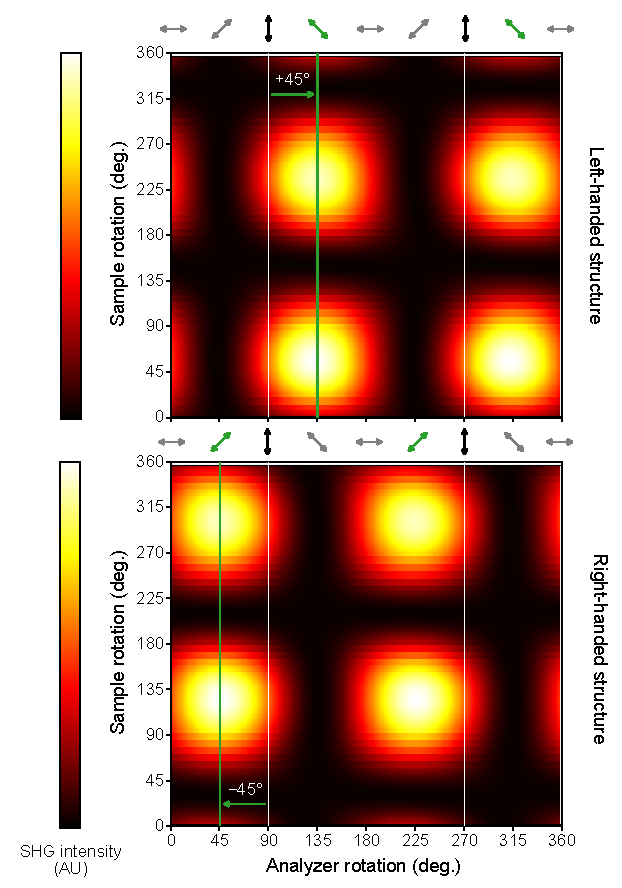
\includegraphics[scale=1]{./figures/results/OAinPlanarNanohelices/sim_data.pdf}

    \caption{\label{fig:results:OAinPlanarNanohelices:sim_data}
    SHG optical rotation heatmaps for the susceptibility tensor relationships given in equation~\ref{eq:results:OAinPlanarNanohelices:ExampleComponents}. The SHG-OR behavior closely matches that observed in Figure~\ref{fig:results:OAinPlanarNanohelices:s_data}.}
\end{figure}

In an \textit{isotropic} metasurface, composed of nanohelices, two principal models can be used to theoretically quantify the nonlinear optical activity. The first model builds upon Kauzmann's ``one-electron chirality''~\cite{Kauzmann1957a}.
In its nonlinear treatment, the nonlinear optical activity requires magnetic dipoles caused by the electron's helical motion.\cite{Hache2001a}
The second model, builds upon Kuhn's~\cite{Kuhn1930} chirally-coupled electric dipole moments. In its nonlinear treatment, the nonlinear optical activity requires only electric dipole moments.\cite{Hache2001a}
In plasmonic nanomaterials this could be the coupling between any chirally-arranged metallic features. Importantly, the ``one-electron'' model permits only SHG-CID, whereas the coupled-dipole model allows SHG-CID, SHG linear dichroism (SHG-LD), and SHG-OR.\cite{Fischer2005a}
Unlike linear chiroptical measurements, information is gained by measuring both SHG-CID and SHG-OR: the mechanism of a structure's chiroptical response can be determined by comparing these two nonlinear chiroptical effects. 

However, when treating \textit{anisotropic} surfaces, the analysis is much more complex than in the isotropic case. SHG-OR is possible in both models, and there is no simple distinction between the two. Slight changes in the structure design can result in significant changes in the optical behavior, due to the large number of interacting tensor components responsible for the SHG-OR. As we have observed, this complexity can result in interesting and highly desirable optical properties, under the right experimental and geometric conditions. The flexibility of geometry makes metamaterials an ideal platform for exploring this interplay between structural and experimental geometry. 

Finally, it is important to consider that the SHG-OR in Figure~\ref{fig:results:OAinPlanarNanohelices:s_data} could, in principle, originate from the out of plane anisotropy axis. SHG-OR effects from this axis would not change under azimuthal sample rotation. However, such an anisotropy-induced SHG-OR would not change sign, depending on the handedness of the nanohelices. Consequently, because our SHG-OR changes sign depending on handedness, we can conclusively attribute it to chirality. 

\section{Conclusions}\label{sec:results:OAinPlanarNanohelices:conclusions}
To conclude, this chapter reports a large SHG-OR effect of $\pm \SI{45}{\deg}$ from planar chiral metamaterials. The effect is due to the intrinsic chirality of the helical nanostructures; the angle of SHG-OR is rotationally invariant, and, as expected, it reverses for the mirrored structures. Contrary to their linear chiroptical counterparts, SHG-CID and SHG-OR are not trivially related to one another. Therefore, these results pertain to an important and previously unobserved chiroptical effect in this kind of system. We have demonstrated that, under specific experimental conditions, it is possible to extract purely chiral information from highly anisotropic structures. Further work on disentangling chiral and anisotropic contributions to nonlinear chiroptical effects will unveil the physical mechanisms at work and will lead to their optimization. 
\chapter{Optical Activity in Hyper-Rayleigh Scattering}\label{sec:results:HRS}
\section{Introduction}

\begin{figure}[htb!]	
    \centering	
    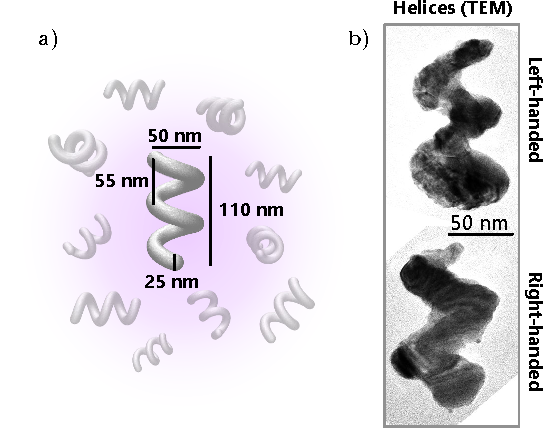
\includegraphics[scale=1]{./figures/results/HRS/sample_schematic.pdf}
    \caption{\label{fig:results:HRS:sample_schematic}
    \textbf{a)} Dimensions (center-to-center) of the nanohelices isotropically dispersed in water. Helix height is $\SI{110}{\nano\m}$, loop diameter is $\SI{50}{\nano\m}$, loop pitch is $\SI{55}{\nano\m}$, and wire-diameter is $\SI{25}{\nano\m}$. \textbf{b)} Transmission Electron Microscopy (TEM) images of left- and right-handed helices. }	
\end{figure}

\begin{figure}[htb!]	
    \centering	
    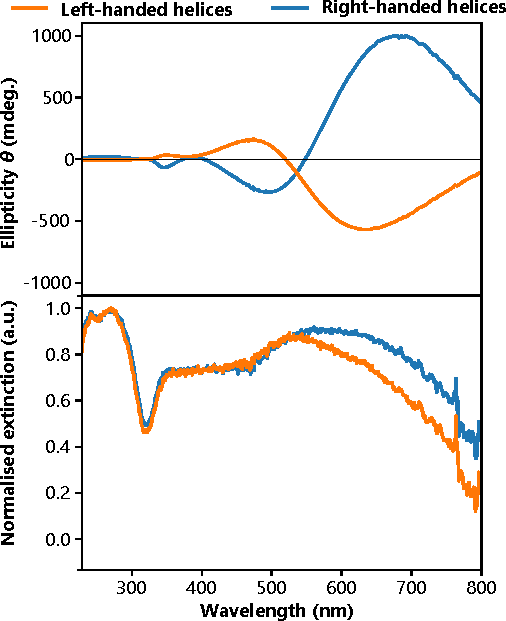
\includegraphics[scale=1]{./figures/results/HRS/linear_data.pdf}
    \caption{\label{fig:results:HRS:linear_data}
    Linear characterization of the nanohelix solutions. Left: ellipticity spectra, as measured with a CD spectrometer, through a $\SI{1}{\centi\m}$ path length filled with left- and right-handed nanohelix suspensions. Right: corresponding normalized extinction spectra from the left- and right-handed nanohelix suspensions. Extinction is obtained from the transmission spectrum and describes both absorption and scattering losses.}	
\end{figure}

\section{Results}

\begin{figure}[htb!]	
    \centering	
    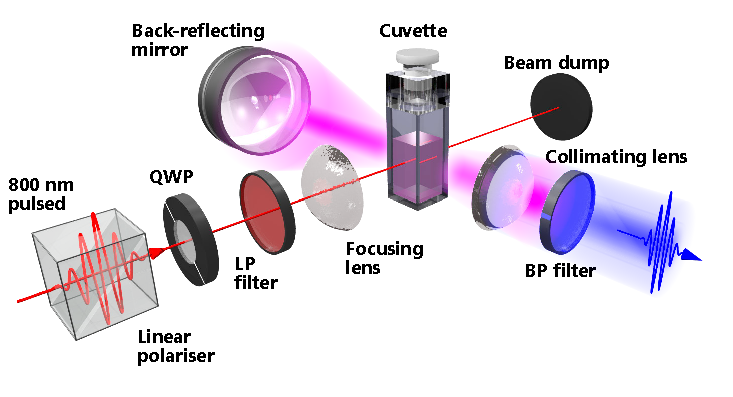
\includegraphics[scale=1]{./figures/results/HRS/experiment_schematic.pdf}
    \caption{\label{fig:results:HRS:experiment_schematic}
    Schematic diagram of the hyper-Rayleigh scattering circular dichroism experimental setup. QWP: quarter wave-plate; LP filter: long-pass filter; BP filter: band pass filter. }	
\end{figure}

\begin{figure}[htb!]	
    \centering	
    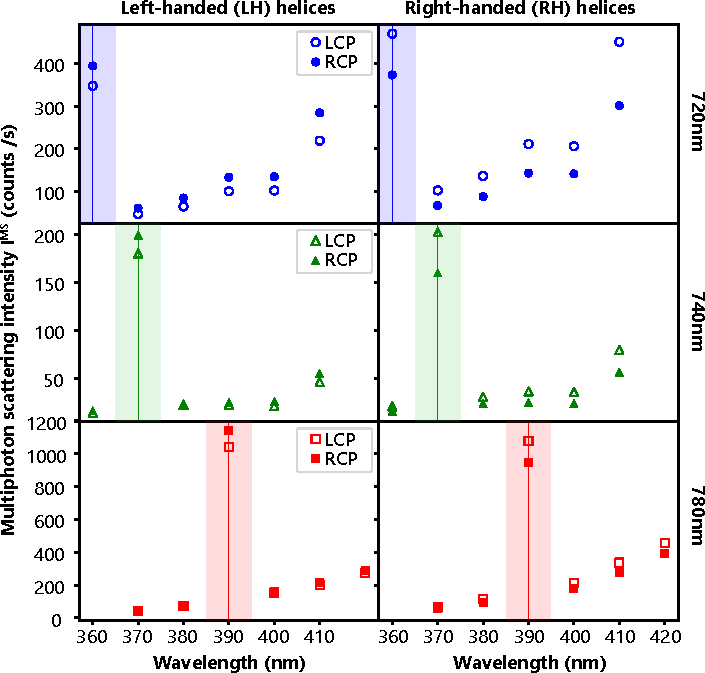
\includegraphics[scale=1]{./figures/results/HRS/hrs_data.pdf}
    \caption{\label{fig:results:HRS:hrs_data}
    Multi-photon scattering spectra for left- and right-handed helices, under LCP and RCP illumination. Results obtained for fundamental wavelengths of $\SI{720}{\nano\m}$, $\SI{740}{\nano\m}$ and $\SI{780}{\nano\m}$ are shown in blue, green, and red, respectively. Vertical colored lines mark the HRS (second-harmonic) wavelength, demonstrating clear peaks above the multiphoton luminescence background. The HRS unambiguously follows variations of the fundamental. }	
\end{figure}

\begin{figure}[htb!]	
    \centering	
    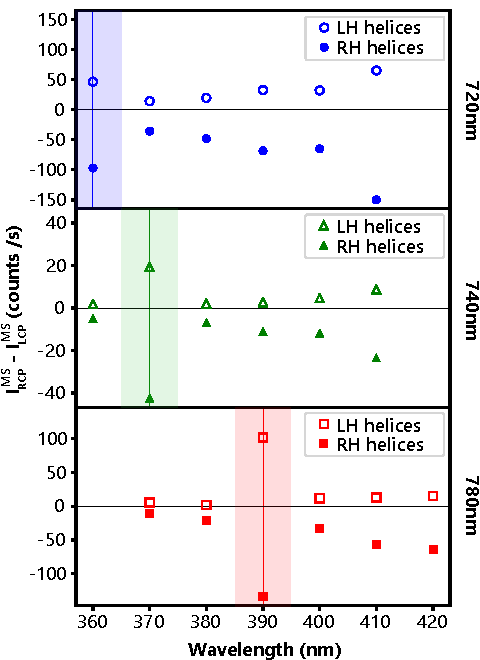
\includegraphics[scale=1]{./figures/results/HRS/hrs_cd_data.pdf}
    \caption{\label{fig:results:HRS:hrs_cd_data}
    Circular difference ($I_{RCP}^{MS}-I_{LCP}^{MS}$) in multiphoton scattering intensity, for both left-handed (LH) and right-handed (RH) nanohelix suspensions. Again, pump wavelengths of $\SI{720}{\nano\m}$, $\SI{740}{\nano\m}$ and $\SI{780}{\nano\m}$ are shown in blue, green, and red, respectively, and vertical coloured lines mark the HRS (second-harmonic) wavelength. The HRS circular difference clearly reverses between nanohelix enantiomorphs.}	
\end{figure}

\begin{table}[tbp]
    \begin{tabular}{llll}
    \firsthline
                                                                & \textbf{\begin{tabular}[c]{@{}l@{}}Fundamental \\ wavelength (nm)\end{tabular}} & \textbf{\begin{tabular}[c]{@{}l@{}}Linear \\ ellipticity (mdeg.)\end{tabular}} & \textbf{\begin{tabular}[c]{@{}l@{}}HRS \\ ellipticity (mdeg.)\end{tabular}} \\ 
    \hline
    \multirow{3}{*}{\begin{tabular}[c]{@{}l@{}}Right-handed \\ helices\end{tabular}}  & 720                                                                    & 920                                                                   & -3299                                                              \\
                                                                & 740                                                                    & 803                                                                   & -3356                                                              \\
                                                                & 780                                                                    & 569                                                                   & -1890                                                              \\ 
    \hline
    \multirow{3}{*}{\begin{tabular}[c]{@{}l@{}}Left-handed \\ helices\end{tabular}}& 720                                                                    & -370                                                                  & 1811                                                               \\
                                                                & 740                                                                    & -293                                                                  & 1455                                                               \\
                                                                & 780                                                                    & -164                                                                  & 1334                                                               \\ 
    \lasthline
    \end{tabular}
    \caption{Linear and HRS ellipticities for left- and right-handed nanohelix suspensions. Values are given at the three fundamental wavelengths used in the HRS experiments.}
    \label{table:HRS:ellipticity}
\end{table}

\begin{figure}[htb!]	
    \centering	
    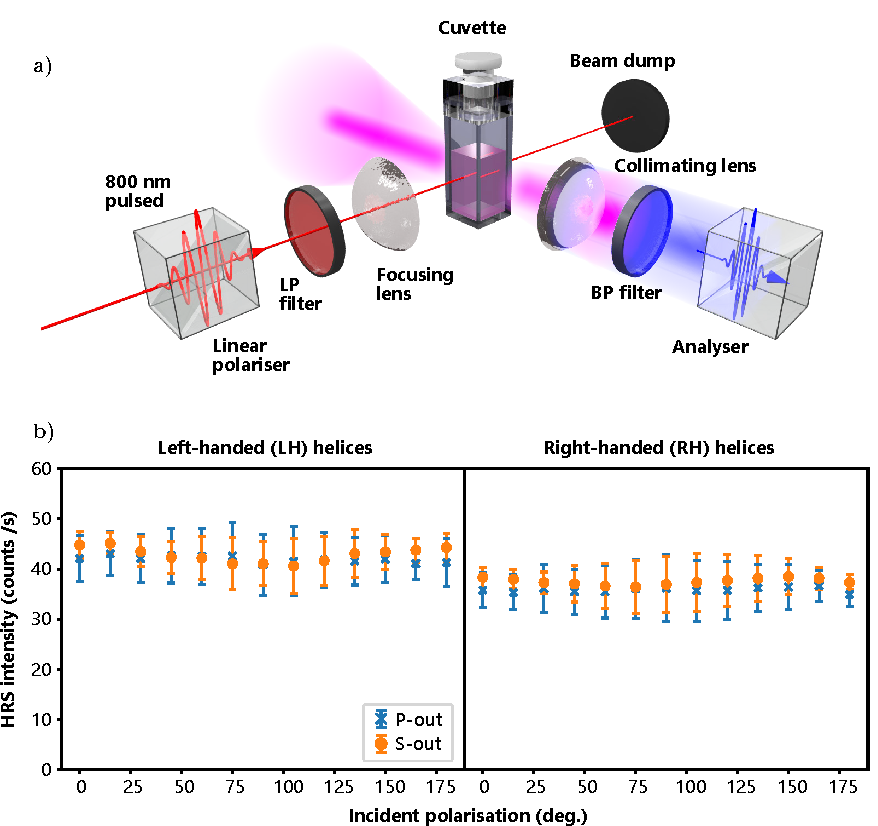
\includegraphics[scale=1]{./figures/results/HRS/hrs_linpol_data.pdf}
    \caption{\label{fig:results:HRS:hrs_linpol_data}
    The nanohelices are isotropically suspended in water. \textbf{a)} Schematic of the setup used to measure hyper-Rayleigh scattering of linearly polarised incident light. \textbf{b)} P-polarised (blue crosses) and S-polarised (orange dots) HRS intensity at $\SI{360}{\nano\m}$, as the polarization of $\SI{720}{\nano\m}$ incident light is rotated. Both left-handed (LH) and right-handed (RH) nanohelix suspensions exhibit no variation outside of experimental uncertainty, demonstrating a clear isotropic arrangement of helices within the liquid suspension.}	
\end{figure}

\section{Discussion}
\section{Conclusions}

\chapter{Summary and Conclusions}\label{sec:Conclusions}

With the availability of modern nanofabrication techniques, chiral plasmonic nanomaterials, in particular, have opened up the field of nanophotonics to a wide range of novel devices. By optimising structural chirality parameters, negative index metamaterials have been realised, with applications in sub-wavelength imaging. Similar effects have also been utilised for ultra-thin polarisation optics. Perhaps more surprisingly, chiral plasmonic devices have also introduced a new platform for nanorobotics. Key to perhaps more humanitarian applications however is the possibility to realise new, sensitive chemical characterisation techniques for the pharmaceutical and biochemistry industries. 

Development within these research areas, and more, has been rapidly accelerated by development in nanofabrication techniques, and the unparalleled freedom that comes with the use of nanomaterials. By lifting limits on the nanomaterial geometries available for fabrication, limits on the optical effects available for exploration are correspondingly lifted. In many cases however, the diversity of nanomaterial characterisation experiments has not yet matched the diversity of material geometries available: Many ``off-the-shelf'' experimental techniques are not necessarily perfectly suited to the characterisation of particular nanomaterial geometries. This work has focused on developing experimental techniques designed for the characterisation of chiral nanomaterials fabricated by our collaborators, by specifically considering the unique properties of each, and the experimental challenges these properties may present. 

Common to each of the samples studied is the comprehensive use of second-harmonic nonlinear optical effects as probes for chirality. Second-harmonic chiroptical effects have been shown to function as highly sensitive probes for chirality, due to the symmetry sensitivity of second-harmonic generation. In experiments characterising chiral structures within an achiral background, SHG is generally forbidden from the achiral bulk, thus providing intrinsic background reduction. Furthermore, and contrary to linear optical counterparts, SHG chiroptical effects are permitted within the electric dipole approximation, providing entirely new information due to their fundamentally different physical origin. By utilising these various enhancements, we have demonstrated a set of analysis techniques for three very different chiral plasmonic nanomaterials.

Plasmonic structure arrays with dimensions comparable to the wavelength of light can support higher order plasmon modes, whose spatial profiles directly relate to the material geometry. We have shown that by examining intermediate geometries between opposite enantiomorphs, unexpected optical behaviour can be observed. Electric field hotspots form at the centre of our chiral cross structures, originating from higher order hybridized plasmon modes of the coupled nanostripes composing the crosses. Structural chirality directly leads to a circular difference in the hotspot intensity, which was measured using SHG microscopy. By considering modal decompositions of the total plasmonic responses, new avenues for chiroptical optimization are opened. By tuning the structure geometry, or introducing auxiliary processes that modify the coupling strengths of specific modes, the chiroptical response can be enhanced by suppressing contributions from the ``wrong'' modes.

In many such planar nanomaterials, structural anisotropy can ``dilute'' chiroptical measurements, making it difficult to extract pure chiral information over contributions from anisotropy. Previous work has shown that in a helical metamaterial, nonlinear circular intensity difference effects are dominated by structural anisotropy. By instead measuring SHG optical rotation from same helical metamaterial, we have shown that, under specific experimental conditions, it is possible to obtain a chiroptical response that provides separable information about chirality and anisotropy. The conditions depend strongly on both the nanomaterial geometry, and the illumination conditions. Changing, for instance, the polarisation of incident light resulted in a response completely dominated by anisotropy, with no separable chiral information available. Nevertheless, the work demonstrated, for the first time, SHG optical rotation from a chiral metamaterial, which can be exclusively attributed to intrinsic chirality. Carefully selecting the experimental geometry for a particular sample geometry can generally allow for more comprehensive chiral characterisation of anisotropic metamaterials in the future.

Finally, we examined the case of intrinsically removing anisotropy from the experimental system, by suspending randomly oriented silver nanohelices in liquid. In our previous experiments, nonlinear chiroptical effects could be measured by detecting SHG in a reflection geometry. For liquid samples, we employed a hyper-Rayleigh scattering (HRS) geometry, to measure the circular difference in second-harmonic scattering of incident light. Strong HRS circular intensity difference was observed at three different incident wavelengths, well above background. Within the electric dipole approximation, HRS-CID is symmetry forbidden. Our observations can be explained by both magnetic dipole contributions to HRS, and the helices behaving as helical arrangements of coupled dipoles, rather than as point scatterers themselves. Future experiments outside of the scope of this thesis may be able to determine the dominant of these contributions to the observed HRS-CID. In this work we have nevertheless reported the first experimental observation of HRS-CID in a liquid sample, providing pure chiral information independent of the individual nanohelices anisotropy.

As our understanding of chirality in nanophotonics develops, and nanofabrication techniques open up even more design flexibility, it should be expected that the need for tailored characterisation experiments will blossom. It seems only reasonable that the freedom and creativity permitted by modern nanofabrication should be matched by novel detection and characterisation schemes. Throughout this project, we have demonstrated a range of techniques designed to reveal previously unobserved behaviour from particular nanomaterial samples. By more fully exploiting the level of freedom permitted by such systems, the field of chiral nanophotonics will no doubt benefit from specially tailored characterisation techniques in the future, allowing for more rapid design, characterisation, and enhancement of chiral optical nanomaterials.


% Bibliography
%\bibliographystyle{unsrt}
\bibliographystyle{ieeetr}
\bibliography{library}
\clearpage

% Appendix
\appendix
\chapter{Reducing \texorpdfstring{$\chi^{(2)}$}{Lg} with Symmetry}\label{sec:appendix:rotations}
\section{4-fold Rotational Symmetry}\label{sec:appendix:rotations:4foldRot}

For a rotation of $\theta=\frac{\pi}{2}$, the transformation matrix is given by

\begin{equation}\label{eq:pi/2RotationMatrix}
	R(\theta=\frac{\pi}{2})_{i,j} =
	\begin{bmatrix}
		0 & -1 & 0\\ 
		1 & 0 & 0\\ 
		0 & 0 & 1
	\end{bmatrix}
\end{equation}
We apply the rotation to $\chi_{ijk}$ given in equation~\ref{eq:background:NonlinearOptics:shgP:chiFull}, as in equation~\ref{eq:background:NonlinearOptics:rotation:RotateChi}, giving
\begin{equation}\label{eq:ChiFull4fold}
	\chi_{ijk}^{\prime} =
	\begin{bmatrix}
		-\chi_{yyy} & -\chi_{yxx} & -\chi_{yzz} & -\chi_{yxz} & -\chi_{yzx} & \chi_{yzy} & \chi_{yyz} & \chi_{yyx} & \chi_{yxy}\\ 
		\chi_{xyy} & \chi_{xxx} & \chi_{xzz} & \chi_{xxz} & \chi_{xzx} & -\chi_{xzy} & -\chi_{xyz} & -\chi_{xyx} & -\chi_{xxy}\\ 
		\chi_{zyy} & \chi_{zxx} & \chi_{zzz} & \chi_{zxz} & \chi_{zzx} & -\chi_{zzy} & -\chi_{zyz} & -\chi_{zyx} & -\chi_{zxy}
	\end{bmatrix}
\end{equation}
By enforcing the symmetry $\chi_{ijk}^{\prime}=\chi_{ijk}$, we find that 7 independent components remain, leaving
\begin{equation}\label{eq:4foldChi}
	\chi^{(2)}_{ijk} =
	\begin{bmatrix}
		0 & 0 & 0 & \chi_{xyz} & \chi_{xzy} & \chi_{xzx} & \chi_{xxz} & 0 & 0\\ 
		0 & 0 & 0 & \chi_{yyz} & \chi_{yzy} & \chi_{yzx} & \chi_{yxz} & 0 & 0\\ 
		\chi_{zxx} & \chi_{zyy} & \chi_{zzz} & 0 & 0 & 0 & 0 & \chi_{zxy} & \chi_{zyx}
	\end{bmatrix}
\end{equation}
with dependencies given by
\begin{equation}\label{eq:4foldDependancies}
\begin{split}
	&\chi_{xyz} = -\chi_{yxz}, \chi_{xzy} = -\chi_{yzx}, \chi_{xzx} = \chi_{yzy} \\
	&\chi_{xxz} = \chi_{yyz}, \chi_{zxx} = \chi_{zyy}, \chi_{zxy} = -\chi_{zyx} \\
	&\chi_{zzz}
\end{split}
\end{equation}
Applying permutation symmetry leaves the reduced tensor as
\begin{equation}\label{eq:Reduced4fold}
	d_{il} = 
	\begin{pmatrix}
		0 & 0 & 0 & \chi_{xyz} & \chi_{xzx} & 0\\ 
		0 & 0 & 0 & \chi_{yzy} & \chi_{yzx} & 0\\ 
		\chi_{zxx} & \chi_{zyy} & \chi_{zzz} & 0 & 0 & 0
	\end{pmatrix} 
\end{equation}
with dependencies $\chi_{xyz} = -\chi_{yzx}$, $\chi_{yzy} = \chi_{xzx}$, and $\chi_{zxx} = \chi_{zyy}$.


\section{2-fold Rotational Symmetry}\label{sec:appendix:rotations:2foldrot}

In the case of 2-fold rotational symmetry around the z axis, the appropriate rotation matrix is given by equation~\ref{eq:background:NonlinearOptics:rotation:AllRotationMatrices} as
\begin{equation}\label{eq:piRotationMatrix}
	R(\theta=\pi)_{i,j} =
	\begin{bmatrix}
		-1 & 0 & 0\\ 
		0 & -1 & 0\\ 
		0 & 0 & 1
	\end{bmatrix}
\end{equation}
This corresponds to the coordinate substitution $x\rightarrow-x$, $y\rightarrow-y$, $z\rightarrow z$. Again, applying rotation to $\chi_{ijk}$ and enforcing the symmetry $\chi_{ijk}^{\prime}=\chi_{ijk}$ leaves the reduced tensor
\begin{equation}\label{eq:2foldChi}
	\chi^{(2)}_{ijk} =
	\begin{bmatrix}
		0 & 0 & 0 & \chi_{xyz} & \chi_{xzy} & 0 & 0 & \chi_{xxy} & \chi_{xyx}\\ 
		\chi_{yxx} & \chi_{yyy} & \chi_{yzz} & 0 & 0 & \chi_{yzx} & \chi_{yxz} & 0 & 0\\ 
		0 & 0 & 0 & \chi_{zyz} & \chi_{zzy} & 0 & 0 & \chi_{zxy} & \chi_{zyx}
	\end{bmatrix}
\end{equation}
with all remaining components left independent~\cite{Boyd2008a}. 

\section{3-fold Rotational Symmetry}\label{sec:appendix:rotations:3foldrot}

The case of 3-fold rotational symmetry is more complex, since for a rotation of $\theta=\frac{2}{3}\pi$ radians the rotation matrix is given by
\begin{equation}\label{eq:2pi/3RotationMatrix}
	R(\theta=\frac{2}{3}\pi)_{i,j} =
	\begin{bmatrix}
		-\frac{1}{2}x & -\frac{\sqrt{3}}{2} & 0\\ 
		\frac{\sqrt{3}}{2} & -\frac{1}{2} & 0\\ 
		0 & 0 & 1
	\end{bmatrix}
\end{equation}
As before, we can rotate $\chi_{ijk}$ and equate to the initial tensor, giving
\begin{equation}\label{eq:RotateChi3fold}
	\chi^{\prime}_{ijk} =  
	R(\theta_{z})_{i\alpha} 
	R(\theta_{z})_{j\beta}
	R(\theta_{z})_{k\gamma}
	\chi^{(2)}_{\alpha \beta \gamma} =
	\chi_{ijk}
\end{equation}
This leaves the reduced tensor as
\begin{equation}\label{eq:3foldChi}
	\chi^{(2)}_{ijk} =
	\begin{bmatrix}
		\chi_{xxx} & \chi_{xyy} & 0 & \chi_{xyz} & \chi_{xzy} & \chi_{xzx} & \chi_{xxz} & \chi_{xxy} & \chi_{xyx}\\ 
		\chi_{yxx} & \chi_{yyy} & 0 & \chi_{yyz} & \chi_{yzy} & \chi_{yzx} & \chi_{yxz} & \chi_{yxy} & \chi_{yyx}\\ 
		\chi_{zxx} & \chi_{zyy} & \chi_{zzz} & 0 & 0 & 0 & 0 & \chi_{zxy} & \chi_{zyx}
	\end{bmatrix}
\end{equation}
with the dependencies 
\begin{equation}\label{eq:3foldDependancies}
\begin{split}
	&\chi_{xxx} = -\chi_{xyy} = -\chi_{yyz} = -\chi_{yxy}\\
	&\chi_{xyz} = -\chi_{yxz}, \chi_{xzy} = -\chi_{yzx}\\
	&\chi_{xzx} = \chi_{yzy}, \chi_{xxz} = \chi_{yyz}\\
	&\chi_{yyy} = -\chi_{yxx} = -\chi_{xxy} = -\chi_{xyx}\\
	&\chi_{zxx} = \chi_{zyy}, \chi_{zxy} = -\chi_{zyx}\\
	&\chi_{zzz}
\end{split}
\end{equation}
Under permutation symmetry, this reduces to
\begin{equation}\label{eq:Reduced3fold}
	d_{il} = 
	\begin{pmatrix}
		\chi_{xxx} & \chi_{xyy} & 0 & \chi_{xyz} & \chi_{xzx} & \chi_{xyx}\\ 
		\chi_{yxx} & \chi_{yyy} & 0 & \chi_{yzy} & \chi_{yzx} & \chi_{yxy}\\ 
		\chi_{zxx} & \chi_{zyy} & \chi_{zzz} & 0 & 0 & 0
	\end{pmatrix}
\end{equation}
\chapter{Quantifying chirality}\label{sec:appendix:QuantifyingChirality}
\section{Calculating chiral geometric difference}\label{sec:appendix:ChiralGeoDiff}

To quantify a simple measure of the geometric chirality of a structure, we use the maximum possible overlap of a pair of mirrored structures. An achiral structure can completely overlap with its mirror image after undergoing only rotation and translation. Therefore, a structure with high ``chiral geometric difference'' will have a low maximum overlapping area (or volume) with its mirror image under only rotation and translation. Here, we define our chiral geometric difference as $1 - A_{Overlap} / A_{Total}$,
where $A_{Overlap}$ is the area of maximal overlap that can be achieved between left- and right-handed shapes, and $A_{Total}$ is the total area of both shapes. 
As can be seen in Figure~\ref{fig:results:EnantiomorphingChiralCrosses:setup}b (in the main text), we use the negative of this value for the chiral geometric difference of the opposite enantiomer. Since the overlap cannot be negative, this is done solely for comparison to experimental data.

We calculate $A_{Overlap}$ by rotating and translating the two mirror-image shapes relative to each other, and optimizing these parameters to maximize the overlapping area. Examples of this overlap are given in Figure~\ref{fig:appendix:ChiralGeoDiff}.


\begin{figure}[htb!]	
    \centering	
    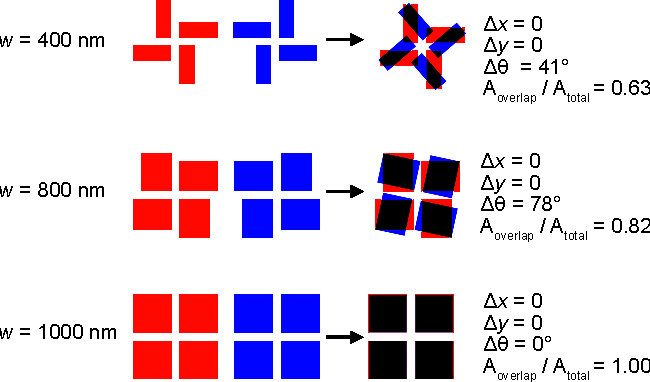
\includegraphics[scale=0.8]{./figures/results/EnantiomorphingChiralCrosses/geoDiff.pdf}
    \caption{\label{fig:appendix:ChiralGeoDiff}
    Examples of the overlap used to define our chiral geometric difference. Red and blue show the right- and left- handed crosses respectively.   $A_{Total}$ is the sum of the red and blue areas. $A_{Overlap}$ is the maximum overlapping area, shown in black. $\Delta x$, $\Delta y$ and $\Delta \theta$ give the parameters for translation ($x$, $y$) and rotation respectively, obtained by maximizing $A_{Overlap}$. In the achiral case ($w=\SI{1000}{\nano\m}$), complete overlap is possible because the structure is achiral. }	
\end{figure}

\end{document}